% LaTeX companion of main.typ. Both formats are editable.
% !TeX program = xelatex
\documentclass{../toolchain/latex/qlnotes-native}
\usepackage{pdflscape}
% Editable TikZ counterpart of probability-diagrams.typ.
% Load TikZ in the preamble, then input this library; call a source diagram by its unchanged
% name, for example \csname prob-02-random-variables-diagram-01\endcsname.
% Coordinates, point radii, colours, formulae and sample counts follow CeTZ.
\ifdefined\ProbDiagramLibraryLoaded\else
\newcommand{\ProbDiagramLibraryLoaded}{}
\ifdefined\tikzpicture\else\RequirePackage{tikz}\fi
\usetikzlibrary{arrows.meta}

\definecolor{probBlue}{HTML}{2574D8}
\definecolor{probDarkBlue}{HTML}{1E5DAD}
\definecolor{probRed}{HTML}{D84B4B}
\definecolor{probOrange}{HTML}{E98A2E}
\definecolor{probGreen}{HTML}{2F9E6F}
\definecolor{probPurple}{HTML}{7950B2}
\definecolor{probGray}{HTML}{667085}
\definecolor{probInk}{HTML}{172033}

\tikzset{
  prob diagram/.style={
    draw=black, line width=1pt,
    >={Triangle[open,length=0.2cm,width=0.15cm]},
    every node/.style={font=\fontsize{7}{8.4}\selectfont,
      text=black, inner sep=0pt, outer sep=0pt},
    baseline=(current bounding box.center)
  },
  prob guide/.style={draw=probGray, dashed},
  prob curve/.style={line width=1.5pt, draw=probBlue}
}

% axes(x-end, y-end, x-label, y-label), in the current coordinate units.
\newcommand{\ProbDiagramAxes}[4]{%
  \draw[->] (-0.2,0) -- (#1,0);
  \draw[->] (0,-0.2) -- (0,#2);
  \node[anchor=west] at (#1,0) {#3};
  \node[anchor=south] at (0,#2) {#4};
}

% covariance-panel(offset, points, trend-start, trend-end, label).
% Points are a comma-separated list of x/y pairs, suitable for \foreach.
\newcommand{\ProbCovariancePanel}[5]{%
  \begin{scope}[shift={(#1,0)}]
    \draw[->] (-0.35,0) -- (3,0);
    \draw[->] (0,-0.35) -- (0,3);
    \foreach \probX/\probY in {#2} {
      \fill[probInk] (\probX,\probY) circle[radius=1.35pt];
    }
    \draw[probRed,dashed] #3 -- #4;
    \node[anchor=center,font=\fontsize{6.5}{7.8}\selectfont]
      at (1.4,-0.5) {#5};
  \end{scope}
}

% Source: prob-01-combinatorics-prob-space-diagram-01().
\expandafter\newcommand\csname prob-01-combinatorics-prob-space-diagram-01\endcsname{%
  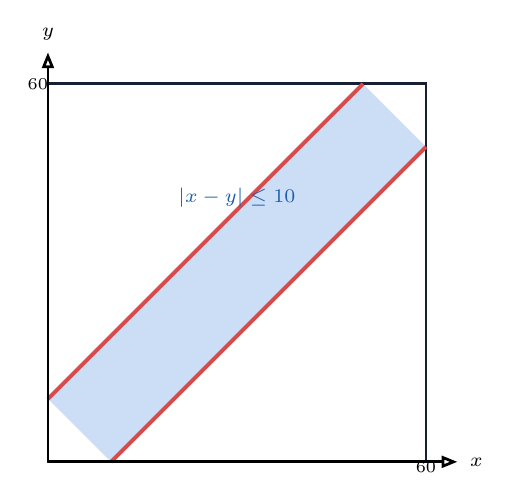
\begin{tikzpicture}[prob diagram,x=0.08cm,y=0.08cm]
    \draw[probInk,line width=1pt] (0,0) -- (0,60) -- (60,60) -- (60,0) -- cycle;
    \fill[probBlue,fill opacity=0.24]
      (0,10) -- (10,0) -- (60,50) -- (50,60) -- cycle;
    \draw[probRed,line width=1.4pt] (10,0) -- (60,50);
    \draw[probRed,line width=1.4pt] (0,10) -- (50,60);
    \draw[->] (0,0) -- (65,0);
    \draw[->] (0,0) -- (0,65);
    \node[anchor=west] at (67,0) {$x$};
    \node[anchor=south] at (0,67) {$y$};
    \node[anchor=north,font=\fontsize{6.5}{7.8}\selectfont] at (60,0) {60};
    \node[anchor=east,font=\fontsize{6.5}{7.8}\selectfont] at (0,60) {60};
    \node[text=probDarkBlue] at (30,42) {$|x-y|\leq 10$};
  \end{tikzpicture}%
}

% Source: prob-02-random-variables-diagram-01().
\expandafter\newcommand\csname prob-02-random-variables-diagram-01\endcsname{%
  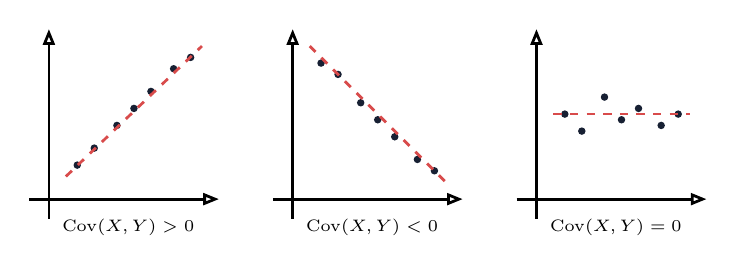
\begin{tikzpicture}[prob diagram,x=0.72cm,y=0.72cm]
    \ProbCovariancePanel{0}
      {0.5/0.6,0.8/0.9,1.2/1.3,1.5/1.6,1.8/1.9,2.2/2.3,2.5/2.5}
      {(0.3,0.4)}{(2.7,2.7)}{$\mathrm{Cov}(X,Y)>0$}
    \ProbCovariancePanel{4.3}
      {0.5/2.4,0.8/2.2,1.2/1.7,1.5/1.4,1.8/1.1,2.2/0.7,2.5/0.5}
      {(0.3,2.7)}{(2.7,0.3)}{$\mathrm{Cov}(X,Y)<0$}
    \ProbCovariancePanel{8.6}
      {0.5/1.5,0.8/1.2,1.2/1.8,1.5/1.4,1.8/1.6,2.2/1.3,2.5/1.5}
      {(0.3,1.5)}{(2.7,1.5)}{$\mathrm{Cov}(X,Y)=0$}
  \end{tikzpicture}%
}

% circular-dependence(): shared by the two original public diagram names.
\newcommand{\ProbCircularDependence}{%
  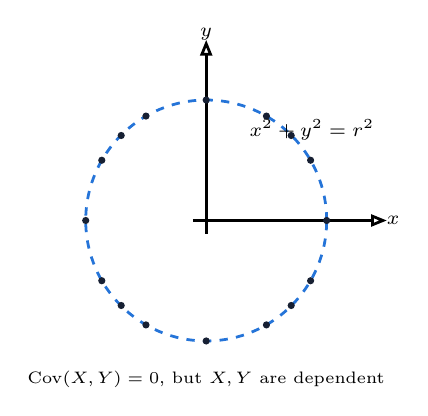
\begin{tikzpicture}[prob diagram,x=0.85cm,y=0.85cm]
    \ProbDiagramAxes{2.7}{2.7}{$x$}{$y$}
    \draw[probBlue,dashed] (0,0) circle[radius=1.8];
    \foreach \probX/\probY in {
      1.8/0,1.27/1.27,0/1.8,-1.27/1.27,
      -1.8/0,-1.27/-1.27,0/-1.8,1.27/-1.27,
      1.56/0.9,0.9/1.56,-0.9/1.56,-1.56/0.9,
      -1.56/-0.9,-0.9/-1.56,0.9/-1.56,1.56/-0.9
    } {
      \fill[probInk] (\probX,\probY) circle[radius=1.3pt];
    }
    \node[anchor=west] at (0.65,1.35) {$x^2+y^2=r^2$};
    \node[anchor=north,font=\fontsize{6.2}{7.44}\selectfont]
      at (0,-2.25) {$\mathrm{Cov}(X,Y)=0$, but $X,Y$ are dependent};
  \end{tikzpicture}%
}

% Source: prob-02-random-variables-diagram-02().
\expandafter\newcommand\csname prob-02-random-variables-diagram-02\endcsname{%
  \ProbCircularDependence
}

% Source: prob-02-random-variables-diagram-03(): Poisson probabilities, lambda=3.
\expandafter\newcommand\csname prob-02-random-variables-diagram-03\endcsname{%
  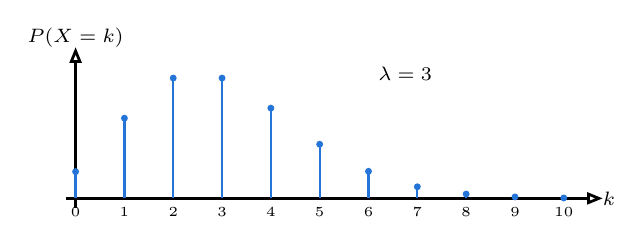
\begin{tikzpicture}[prob diagram,x=0.62cm,y=0.62cm]
    \ProbDiagramAxes{10.8}{3.1}{$k$}{$P(X=k)$}
    \foreach \probP [count=\probK from 0] in {
      0.04979,0.14936,0.22404,0.22404,0.16803,0.10082,
      0.05041,0.02160,0.00810,0.00270,0.00081
    } {
      \pgfmathsetmacro{\probHeight}{11*\probP}
      \draw[probBlue,line width=0.8pt] (\probK,0) -- (\probK,\probHeight);
      \fill[probBlue] (\probK,\probHeight) circle[radius=1.25pt];
      \node[anchor=north,font=\fontsize{5.5}{6.6}\selectfont]
        at (\probK,-0.18) {\probK};
    }
    \node[anchor=west] at (6.2,2.55) {$\lambda=3$};
  \end{tikzpicture}%
}

% Typst's f_X(x)/F_X(x) includes X(x) in the subscript. Preserve the source
% rendering here rather than silently changing that notation during conversion.
% Source: prob-02-random-variables-diagram-04(): uniform density.
\expandafter\newcommand\csname prob-02-random-variables-diagram-04\endcsname{%
  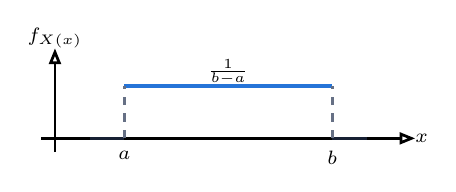
\begin{tikzpicture}[prob diagram,x=0.88cm,y=0.88cm]
    \ProbDiagramAxes{5.2}{1.3}{$x$}{$f_{X(x)}$}
    \draw[probInk,line width=1.2pt] (0.5,0) -- (1,0);
    \draw[prob curve] (1,0.75) -- (4,0.75);
    \draw[probInk,line width=1.2pt] (4,0) -- (4.5,0);
    \draw[prob guide] (1,0) -- (1,0.75);
    \draw[prob guide] (4,0) -- (4,0.75);
    \node[anchor=north] at (1,-0.18) {$a$};
    \node[anchor=north] at (4,-0.18) {$b$};
    \node at (2.5,0.95) {$\frac{1}{b-a}$};
  \end{tikzpicture}%
}

% Source: prob-02-random-variables-diagram-05(): uniform CDF.
\expandafter\newcommand\csname prob-02-random-variables-diagram-05\endcsname{%
  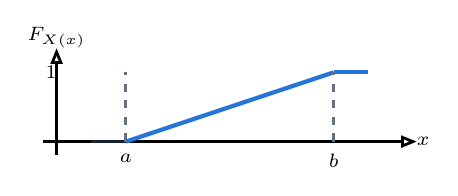
\begin{tikzpicture}[prob diagram,x=0.88cm,y=0.88cm]
    \ProbDiagramAxes{5.2}{1.35}{$x$}{$F_{X(x)}$}
    \draw[probInk,line width=1.2pt] (0.5,0) -- (1,0);
    \draw[prob curve] (1,0) -- (4,1);
    \draw[prob curve] (4,1) -- (4.5,1);
    \draw[prob guide] (1,0) -- (1,1);
    \draw[prob guide] (4,0) -- (4,1);
    \node[anchor=north] at (1,-0.18) {$a$};
    \node[anchor=north] at (4,-0.18) {$b$};
    \node[anchor=east] at (0,1) {$1$};
  \end{tikzpicture}%
}

% Source: prob-02-random-variables-diagram-06().
% Keep the source's plotted exp(-0.5*x) and its general density label verbatim.
\expandafter\newcommand\csname prob-02-random-variables-diagram-06\endcsname{%
  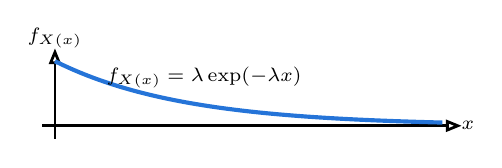
\begin{tikzpicture}[prob diagram,x=0.82cm,y=0.82cm]
    \ProbDiagramAxes{6.3}{1.2}{$x$}{$f_{X(x)}$}
    \draw[prob curve] plot[domain=0:6,samples=81] (\x,{exp(-0.5*\x)});
    \node[anchor=west] at (0.8,0.75) {$f_{X(x)}=\lambda\exp(-\lambda x)$};
  \end{tikzpicture}%
}

% Source: prob-02-random-variables-diagram-07(): exponential CDF.
\expandafter\newcommand\csname prob-02-random-variables-diagram-07\endcsname{%
  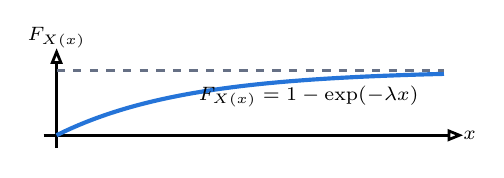
\begin{tikzpicture}[prob diagram,x=0.82cm,y=0.82cm]
    \ProbDiagramAxes{6.3}{1.35}{$x$}{$F_{X(x)}$}
    \draw[prob curve] plot[domain=0:6,samples=81] (\x,{1-exp(-0.5*\x)});
    \draw[prob guide] (0,1) -- (6,1);
    \node[anchor=west] at (2.2,0.6) {$F_{X(x)}=1-\exp(-\lambda x)$};
  \end{tikzpicture}%
}

% gamma-pdf/gamma-cdf(alpha,x): exact integer-shape formulae from Typst.
\pgfmathdeclarefunction{probGammaPdf}{2}{%
  \pgfmathparse{ifthenelse(#1==1,exp(-#2),
    ifthenelse(#1==2,#2*exp(-#2),
    ifthenelse(#1==3,#2*#2*exp(-#2)/2,
      #2*#2*#2*#2*exp(-#2)/24)))}%
}
\pgfmathdeclarefunction{probGammaCdf}{2}{%
  \pgfmathparse{ifthenelse(#1==1,1-exp(-#2),
    ifthenelse(#1==2,1-(1+#2)*exp(-#2),
    ifthenelse(#1==3,1-(1+#2+#2*#2/2)*exp(-#2),
      1-(1+#2+#2*#2/2+#2*#2*#2/6+#2*#2*#2*#2/24)*exp(-#2))))}%
}

% Source: prob-02-random-variables-diagram-08(): alpha=1,2,3,5; lambda=1.
\expandafter\newcommand\csname prob-02-random-variables-diagram-08\endcsname{%
  \begin{tikzpicture}[prob diagram,x=0.72cm,y=0.72cm]
    \ProbDiagramAxes{8.3}{1.2}{$x$}{$f_{X(x)}$}
    \foreach \probAlpha/\probColor in {1/probBlue,2/probRed,3/probGreen,5/probPurple} {
      \draw[\probColor,line width=1.25pt]
        plot[domain=0.05:8,samples=121] (\x,{probGammaPdf(\probAlpha,\x)});
    }
    \node[anchor=north] at (4.2,-0.35) {Gamma densities, $\lambda=1$};
  \end{tikzpicture}%
}

% Source: prob-02-random-variables-diagram-09(): alpha=1,2,3,5; lambda=1.
\expandafter\newcommand\csname prob-02-random-variables-diagram-09\endcsname{%
  \begin{tikzpicture}[prob diagram,x=0.72cm,y=0.72cm]
    \ProbDiagramAxes{8.3}{1.3}{$x$}{$F_{X(x)}$}
    \foreach \probAlpha/\probColor in {1/probBlue,2/probRed,3/probGreen,5/probPurple} {
      \draw[\probColor,line width=1.25pt]
        plot[domain=0:8,samples=121] (\x,{probGammaCdf(\probAlpha,\x)});
    }
    \draw[prob guide] (0,1) -- (8,1);
    \node[anchor=north] at (4.2,-0.35) {Gamma cdfs, $\lambda=1$};
  \end{tikzpicture}%
}

% Source: prob-03-joint-conditional-distribution-diagram-01().
\expandafter\newcommand\csname prob-03-joint-conditional-distribution-diagram-01\endcsname{%
  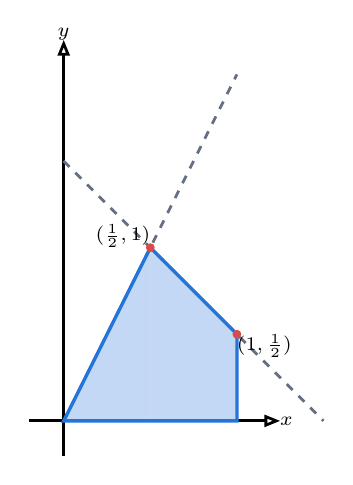
\begin{tikzpicture}[prob diagram,x=2.2cm,y=2.2cm]
    \ProbDiagramAxes{1.25}{2.2}{$x$}{$y$}
    \draw[prob guide] (0,0) -- (1,2);
    \draw[prob guide] (0,1.5) -- (1.5,0);
    \fill[probBlue,fill opacity=0.28] (0,0) -- (0.5,0) -- (0.5,1) -- cycle;
    \fill[probBlue,fill opacity=0.28]
      (0.5,0) -- (1,0) -- (1,0.5) -- (0.5,1) -- cycle;
    \draw[probBlue,line width=1.2pt]
      (0,0) -- (0.5,1) -- (1,0.5) -- (1,0) -- cycle;
    \fill[probRed] (0.5,1) circle[radius=1.6pt];
    \fill[probRed] (1,0.5) circle[radius=1.6pt];
    \node[anchor=south east] at (0.5,1) {$(\frac{1}{2},1)$};
    \node[anchor=north west] at (1,0.5) {$(1,\frac{1}{2})$};
  \end{tikzpicture}%
}

% Source: prob-03-joint-conditional-distribution-diagram-02().
\expandafter\newcommand\csname prob-03-joint-conditional-distribution-diagram-02\endcsname{%
  \ProbCircularDependence
}

% Source: prob-03-joint-conditional-distribution-diagram-03().
\expandafter\newcommand\csname prob-03-joint-conditional-distribution-diagram-03\endcsname{%
  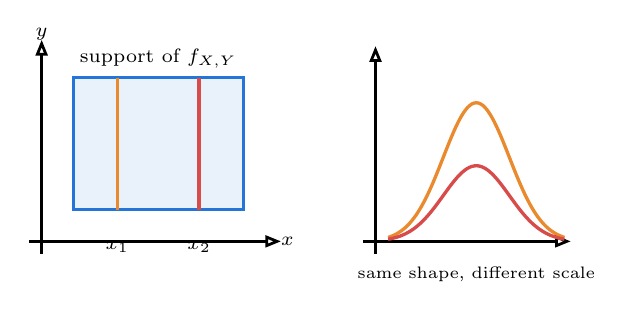
\begin{tikzpicture}[prob diagram,x=0.8cm,y=0.8cm]
    \ProbDiagramAxes{3.8}{3.2}{$x$}{$y$}
    \filldraw[fill=probBlue,fill opacity=0.1,draw=probBlue,
      draw opacity=1,line width=1pt]
      (0.5,0.5) -- (0.5,2.6) -- (3.2,2.6) -- (3.2,0.5) -- cycle;
    \draw[probOrange,line width=1.2pt] (1.2,0.5) -- (1.2,2.6);
    \draw[probRed,line width=1.2pt] (2.5,0.5) -- (2.5,2.6);
    \node[anchor=north] at (1.2,0) {$x_1$};
    \node[anchor=north] at (2.5,0) {$x_2$};
    \node at (1.85,2.9) {support of $f_{X,Y}$};
    \draw[->] (5.1,0) -- (8.4,0);
    \draw[->] (5.3,-0.2) -- (5.3,3.1);
    \draw[probOrange,line width=1.2pt]
      plot[domain=0.2:3,samples=81] ({5.3+\x},{2.2*exp(-((\x-1.6)*(\x-1.6))/0.55)});
    \draw[probRed,line width=1.2pt]
      plot[domain=0.2:3,samples=81] ({5.3+\x},{1.2*exp(-((\x-1.6)*(\x-1.6))/0.55)});
    \node[anchor=north,font=\fontsize{6.5}{7.8}\selectfont]
      at (6.9,-0.4) {same shape, different scale};
  \end{tikzpicture}%
}

% Source: prob-04-lln-diagram-01(): shaded right tail.
\expandafter\newcommand\csname prob-04-lln-diagram-01\endcsname{%
  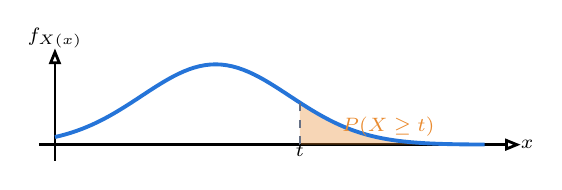
\begin{tikzpicture}[prob diagram,x=1.02cm,y=1.02cm]
    \ProbDiagramAxes{5.8}{1.2}{$x$}{$f_{X(x)}$}
    \fill[probOrange,fill opacity=0.35]
      (3.05,0) -- plot[domain=3.05:5.35,samples=81]
        (\x,{exp(-((\x-2)*(\x-2))/1.7)}) -- (5.35,0) -- cycle;
    \draw[probBlue,line width=1.4pt] plot[domain=0:5.35,samples=81]
      (\x,{exp(-((\x-2)*(\x-2))/1.7)});
    \draw[prob guide] (3.05,0) -- (3.05,{exp(-((3.05-2)*(3.05-2))/1.7)});
    \node[anchor=north] at (3.05,0) {$t$};
    \node[text=probOrange] at (4.15,0.22) {$P(X\geq t)$};
  \end{tikzpicture}%
}
\fi

\title{Math 525: Probability}
\subtitle{Typst-first course notes}
\author{Qiulin Fan}
\date{2026}
\begin{document}
\frontmatter
\maketitle
\tableofcontents
\mainmatter
% LaTeX companion of 01-combinatorics&prob_space.typ. Both formats are editable.
\chapter{basic combinatorics and probability space}\label{basic-combinatorics-and-probability-space}

\section{permutations and combinations}\label{permutations-and-combinations}

\subsection{permutations}\label{permutations}

\begin{definition}{\kn{permutations}}

一个 permutation 就是对一组 objects 的一个 \textbf{rearrangement} (这些 objects 中可以有 same 的也可以有 distinct 的).\\
对于 \(\mathit{n}\) 个 \textbf{distinct objects}, 一共存在

\[\mathit{n}! = \mathit{n}(\mathit{n} - 1)(\mathit{n} - 2)\cdots\]

个 permutations.

\end{definition}

\begin{example}

求 "STATISTICS" 的 \# distinct permutations.

\end{example}

\begin{qlsolution}{Solution}

这里一共有 10 个 objects. 但问题是: 其中有 3 个 \(\mathit{S}\), 3 个 \(\mathit{T}\), 2 个 \(\mathit{I}\) 是相同的.\\
于是: 我们首先假设它们都是 distinct 的, 则存在 \(10!\) 个 permutations. 而, 每个 permutation 都包含了对 3 个 \(\mathit{S}\) 的一个子 permutation. 而对 3 个 \(\mathit{S}\) 的任意 permutation 都是相同的! 同样的道理 apply to 3 个 \(\mathit{T}\) 和 2 个 \(\mathit{I}\).\\
所以这个结果是真实结果的 \(3!3!2!\) 倍.\\
同样地, 由于 因而, 正确结果是:

\[\frac{10!}{3!3!2!1!1!}\]

\end{qlsolution}

\begin{qlremark}{Remark}

求一组 objects 的 distinct permutations 的数量时, 对于其中相同的 objects, 我们只需要除去它们的重复数量的 factorial (即: 它们自己内部有多少个 permutation 都算作一个 permutation).\\
公式:

\[\frac{\mathit{n}!}{\mathit{n}_{1}!\mathit{n}_{2}!\cdots\mathit{n}_{\mathit{k}}!}\]

其中 \(\mathit{n}_{1},\mathit{n}_{2},\cdots,\mathit{n}_{\mathit{k}}\) 是每个 object 的重复数量.\\
这个式子又叫做 multinomial coefficient.

\begin{definition}{\kn{multinomial coefficient}}

令 \(\mathit{n} \in \mathbb{N},\mathit{n}_{1},\mathit{n}_{2},\cdots,\mathit{n}_{\mathit{k}} \in \mathbb{N},\mathit{n}_{1} + \mathit{n}_{2} + \cdots + \mathit{n}_{\mathit{k}} = \mathit{n}\), 我们定义 multinomial coefficient:

\[\binom{\mathit{n}}{\mathit{n}_{1},\mathit{n}_{2},\cdots,\mathit{n}_{\mathit{k}}} = \frac{\mathit{n}!}{\mathit{n}_{1}!\mathit{n}_{2}!\cdots\mathit{n}_{\mathit{k}}!}\]

\end{definition}

\begin{proposition}

如果我们需要 \(\mathit{n}_{1}\) 个 object 1, \(\mathit{n}_{2}\) 个 object 2, \(\cdots\), \(\mathit{n}_{\mathit{k}}\) 个 object \(\mathit{k}\), 那么它们的 distinct permutations 的数量为:

\[\binom{\mathit{n}_{1} + \mathit{n}_{2} + \cdots + \mathit{n}_{\mathit{k}}}{\mathit{n}_{1},\mathit{n}_{2},\cdots,\mathit{n}_{\mathit{k}}}\]

\end{proposition}

\end{qlremark}

\subsection{combinations}\label{combinations}

\begin{definition}{\kn{combinations}}

一个 combination 就是从一个 set 中选取若干个 elements, 而忽略它们的顺序.

\end{definition}

\begin{proposition}

从 \(\mathit{n}\) 个 \textbf{distinct objects} 中选取 \(\mathit{k}\) 个的 combinations 的数量为:

\[\binom{\mathit{n}}{\mathit{k}} = \frac{\mathit{n}!}{\mathit{k}!(\mathit{n} - \mathit{k})!}\]

\end{proposition}

\begin{proof}

我们可以将问题转化为: 从 \(\mathit{n}\) 个 \textbf{distinct objects} 中选取 \(\mathit{k}\) 个的 permutations 的数量, 然后再除去重复的 permutations. 而, 从 \(\mathit{n}\) 个 \textbf{distinct objects} 中选取 \(\mathit{k}\) 个的 permutations 的数量为:

\[\mathit{n} \times (\mathit{n} - 1) \times \cdots \times (\mathit{n} - \mathit{k} + 1) = \frac{\mathit{n}!}{(\mathit{n} - \mathit{k})!}\]

而其中, 对于每个 valid combination, 都包含了它的所有 ordered permutations, 即重复了 \(\mathit{k}!\) 次. 因此, 最终的结果为:

\[\frac{\mathit{n}!}{\mathit{k}!(\mathit{n} - \mathit{k})!}\]

\end{proof}

\subsection{binomial theorem}\label{binomial-theorem}

\begin{theorem}{\kn{Binomial Theorem}}

令 \(\mathit{x},\mathit{y} \in \mathbb{R},\mathit{n} \in \mathbb{N}\), 则有:

\[(\mathit{x} + \mathit{y})^{\mathit{n}} = \sum\limits_{\mathit{k} = 0}^{\mathit{n}}\binom{\mathit{n}}{\mathit{k}}\mathit{x}^{\mathit{n} - \mathit{k}}\mathit{y}^{\mathit{k}}\]

\end{theorem}

\begin{proof}

我们可以 prove this by combiinatorial interpretation. 因为把 \(\mathit{x} + \mathit{y}\) 展开即 \(\mathit{n}\) 个 \((\mathit{x} + \mathit{y})\) 的乘积. 即: 对于每个被乘项, 我们都是在 \(\mathit{x}\) 和 \(\mathit{y}\) 之间选择一个.\\
因而: \(\mathit{x}^{\mathit{k}}\mathit{y}^{\mathit{n} - \mathit{k}}\) 的系数就是从 \(\mathit{n}\) 个 \((\mathit{x} + \mathit{y})\) 中选取 \(\mathit{k}\) 个 \(\mathit{x}\) 的 combinations 的数量, 即 \(\binom{\mathit{n}}{\mathit{k}}\).\\
考虑所有的 possible \(\mathit{k}\) 值, 我们得到:

\[(\mathit{x} + \mathit{y})^{\mathit{n}} = \sum\limits_{\mathit{k} = 0}^{\mathit{n}}\binom{\mathit{n}}{\mathit{k}}\mathit{x}^{\mathit{n} - \mathit{k}}\mathit{y}^{\mathit{k}}\]

这是 combinatorial 的 proof.

\end{proof}

另外一种更轮椅的思路是 prove by induction. 这需要一个辅助的 proposition:

\begin{proposition}

\[\binom{\mathit{n}}{\mathit{k}} = \binom{\mathit{n} - 1}{\mathit{k} - 1} + \binom{\mathit{n} - 1}{\mathit{k}}\]

\end{proposition}

这个等式的 combinatorial interpretation 很 trivial: 对于其中的任意一个 object:

\begin{itemize}
\item
  这个 object 被选中的情况, combinations 的数量: \(\binom{\mathit{n} - 1}{\mathit{k} - 1}\) (从其他里面选 \(\mathit{k} - 1\) 个);
\item
  这个 object 不被选中的情况, combinations 的数量: \(\binom{\mathit{n} - 1}{\mathit{k}}\) (从其他里面选 \(\mathit{k}\) 个).
\end{itemize}

\begin{example}

一个 52-card deck, 取 5 张随机牌, 我们获得:

\begin{itemize}
\item
  4 张同 rank 的牌, 最后一张不同 rank 的牌
\item
  a full house (3 张同 rank 的牌, 2 张同 rank 的牌)
\end{itemize}

的概率是多少?

\end{example}

\begin{qlsolution}{Solution}

一共有 \(\binom{52}{5}\) 种取法. 取 4 张同 rank 的牌: 13 种取法. 取最后一张不同 rank 的牌: 52-4 = 48 种取法. 因而, 概率是:

\[\frac{13 \times 48}{\binom{52}{5}}\]

如果是取 3 张同 rank 的牌 + 两张 different 同 rank 的牌: 我们首先在 4 个花色里面选 3 个, 有 \(\binom{4}{3}\) 种取法.\\
因而选取 3 cards of the same rank 的数量为: \(13 \cdot \binom{4}{3}\).\\
然后选取剩余的两张: 然后故技重施, 从剩下的 12 个 rank 里面选 1 个, 而选择它们的花色有 \(\binom{4}{2}\) 种取法. 因而, 概率是:

\[\frac{13 \cdot \binom{4}{3} \cdot 12 \cdot \binom{4}{2}}{\binom{52}{5}}\]

\end{qlsolution}

\begin{example}

我们有 \(\mathit{n}\) 把钥匙, 其中有一把是正确的. 尝试 \(\mathit{k}\) 次, 能够成功开门的概率是多少?

\end{example}

\begin{qlsolution}{Solution}

一共有 \(\mathit{n}!\) 种钥匙的 permutations. 我们需要的情况: 正确的钥匙出现在前 \(\mathit{k}\) 个位置:

\begin{itemize}
\item
  正确钥匙出现在第 \(1\) 个位置, 其他 \(\mathit{n} - 1\) 随便排列: \(\cdot (\mathit{n} - 1)!\) 种
\item
  \(\cdots\)
\item
  正确钥匙出现在第 \(\mathit{k}\) 个位置, 其他 \(\mathit{n} - 1\) 随便排列: \(\mathit{k} \cdot (\mathit{n} - 1)!\) 种
\end{itemize}

因而正确的 permutations 的数量为:

\[\mathit{k} \cdot (\mathit{n} - 1)!\]

因而, 概率是:

\[\frac{\mathit{k} \cdot (\mathit{n} - 1)!}{\mathit{n}!} = \frac{\mathit{k}}{\mathit{n}}\]

\end{qlsolution}

\begin{qlremark}{Remark}

正确钥匙出现在每个位置上的概率都是 \(1/\mathit{n}\). 因而它出现在前 \(\mathit{k}\) 个位置的概率就是 \(\mathit{k}/\mathit{n}\).\\
这是一类典型的问题: 不放回的抽取. 在只关心"是否在前 \(\mathit{k}\) 次成功"这一事件时, 这个过程等价于"正确钥匙在一个随机排列中的位置". 这一结果只和比例有关, 与过程细节无关. 只要没有信息bias, 没有偏好, 完全随机, 那么成功概率只取决于:

\begin{itemize}
\item
  你允许的尝试次数 \(\mathit{k}\)
\item
  总可能性数 \(\mathit{n}\)
\end{itemize}

而如果是放回则是不同的情况. 通过补事件容易得:

\[\mathbb{P}(\mathit{A}) = 1 - \left( {1 - \frac{1}{\mathit{n}}} \right)^{\mathit{k}}\]

放回和不防回最大的区别是: 放回时, 每次尝试都是独立的, 而不放回时, 每次尝试都不是独立的. 最明显的例子就是, 如果不放回, \(\mathit{k} = \mathit{n}\) 时概率为 1. 而如果放回, 不论 \(\mathit{k}\) 有多大, 概率都小于 1; 当 \(\mathit{k} \ll \mathit{n}\) 的时候, 这两个概率相近 (符合直觉, 因为 \(\mathit{n}\) 很大时放回和不放回几乎没区别.)

\end{qlremark}

\begin{example}

一个篮子里有 \(10\) 个 red balls 和 \(5\) 个 blue balls. 我们随机从中取出 \(3\) 个 balls, exactly 其中 \(1\) 个是 blue ball 的概率是多少? 如果每次都放回呢?

\end{example}

\begin{qlsolution}{Solution}

不放回:

\[\mathbb{P}(\text{exactly one blue ball}) = \binom{10}{2}\binom{5}{1}/\binom{15}{3} = \frac{45}{91}\]

放回: 5 ways to choose the blue ball, 10 ways to choose the red ball, 以及 3 positions to place the blue ball,

\[\mathbb{P}(\text{exactly one blue ball}) = 3 \cdot \frac{3 \cdot 10^{2}}{15^{3}}\]

\end{qlsolution}

\subsection{combinations with repetition}\label{combinations-with-repetition}

\begin{definition}{\kn{combinations with repetition}}

一个 combination with repetition 就是从一个 set 中选取若干个 elements, 而忽略它们的顺序, 并且\textbf{允许重复选取}.

\end{definition}

\begin{proposition}

从 \(\mathit{n}\) 个 \textbf{distinct objects} 中选取 \(\mathit{k}\) 个的 combinations with repetition 的数量为:

\[\binom{\mathit{n} + \mathit{k} - 1}{\mathit{k}}\]

\end{proposition}

\begin{qlremark}{Remark}

关于这个问题我们最开始可能会犯一个错误: 认为 combinations with \(\mathit{k}\) repetitions 的数量为:

\[\binom{\mathit{k}\mathit{n}}{\mathit{k}}\]

但是想一下就知道这是错的. 因为我们相当于给 repeated 的同一个 objects 赋予了顺序, 从而计入了额外的数量.

\end{qlremark}

\begin{proof}

这个问题比较巧妙. 我们上面错误的尝试已经表明: 用 "make copies" 的方法行不通. 我们需要变换一下思路. 原问题是 "要选哪几个元素, 每个元素要选几个". 而我们可以把这个问题理解为: 一共有 \(\mathit{k}\) 个位置, \(\mathit{n}\) 个组, 我们给每个组分配多少个位置?\\
Formalize 这个想法即: 对于第 \(\mathit{i}\) 个 object, 我们给它分配 \(\mathit{x}_{\mathit{i}}\) 个位置. 所有满足条件的 combinations 可以 represent by:

\[\left\{ {\mathit{y} = (\mathit{x}_{1},\mathit{x}_{2},\cdots,\mathit{x}_{\mathit{n}}) \in \mathbb{Z}_{\geq 0}^{\mathit{n}}:\mathit{x}_{1} + \mathit{x}_{2} + \cdots + \mathit{x}_{\mathit{n}} = \mathit{k}} \right\}\]

到这里我们想到一个经典的问题: stars and bars. 即: 把 \(\mathit{k}\) 个星星分成 \(\mathit{n}\) 个组, 每个组至少有 1 个星星. 这个问题等价于: 把 \(\mathit{k}\) 个星星和 \(\mathit{n} - 1\) 个隔板排成一排, 然后选择 \(\mathit{n} - 1\) 个隔板的位置.\\
问题是: 我们这里, 一个组可以有 \(0\) 个 stars; 但是这是小问题. 因为我们可以 set \(\mathit{x}_{\mathit{i}}' = \mathit{x}_{\mathit{i}} + 1\), 问题等价转化为:

\[\left\{ {\mathit{y} = (\mathit{x}_{1}',\mathit{x}_{2}',\cdots,\mathit{x}_{\mathit{n}}') \in \mathbb{Z}_{\geq 1}^{\mathit{n}}:\mathit{x}_{1}' + \mathit{x}_{2}' + \cdots + \mathit{x}_{\mathit{n}}' = \mathit{k} + \mathit{n}} \right\}\]

这就强制每个组至少有一个 star, 于是可以使用 stars and bars 的方法来解决. 即: 用 \(\mathit{n} - 1\) 个隔板隔开 \(\mathit{k} + \mathit{n}\) 个星星 (有 \(\mathit{k} + \mathit{n} - 1\) 个空档). 因而, 满足条件的 combinations 的数量为:

\[\binom{\mathit{k} + \mathit{n} - 1}{\mathit{n} - 1} = \binom{\mathit{k} + \mathit{n} - 1}{\mathit{k}}\]

\end{proof}

\begin{example}

有 5 种口味的 ice creams. 一个人随机选择 20 个 scoops. 求: 每种口味至少被选中一次的 probability.

\end{example}

\begin{qlsolution}{Solution}

即从 \(5\) 种口味中选取 \(20\) 个 combinations with repetition. 于是 sample space 的大小: \(\binom{25 - 1}{20}\).\\
而满足条件的 combinations: 即每种口味我们都预选一个. 然后再从\(5\) 种口味中选取 \(15\) 个 combinations with repetition.

\[\mathbb{P}(\text{each flavor is selected at least once}) = \frac{\binom{19}{15}}{\binom{24}{20}} = \frac{\binom{24}{20}}{\binom{24}{20}}\]

\end{qlsolution}

\subsection{inclusion-exclusion principle}\label{inclusion-exclusion-principle}

\begin{proposition}{\kn{inclusion-exclusion principle}}

如果 \(\Omega\) 是 \knref{measure space} 意义下的一个 finite measure space, 那么对于任意 \(\mathit{A}_{1},\ldots,\mathit{A}_{\mathit{n}} \subseteq \Omega\) 的, 有:

\[\left| {\cup_{\mathit{i} = 1}^{\mathit{n}}\mathit{A}_{\mathit{i}}} \right| = \sum\limits_{\mathit{i} = 1}^{\mathit{n}}\left| \mathit{A}_{\mathit{i}} \right| - \sum\limits_{\mathit{i} < \mathit{j}}\left| {\mathit{A}_{\mathit{i}} \cap \mathit{A}_{\mathit{j}}} \right| + \sum\limits_{\mathit{i} < \mathit{j} < \mathit{k}}\left| {\mathit{A}_{\mathit{i}} \cap \mathit{A}_{\mathit{j}} \cap \mathit{A}_{\mathit{k}}} \right| - \ldots + ( - 1)^{\mathit{n} + 1}\left| {\mathit{A}_{1} \cap \ldots \cap \mathit{A}_{\mathit{n}}} \right|.\]

\end{proposition}

\begin{qlremark}{Remark}

这里的 \(\sum_{\mathit{i} < \mathit{j}}\) 等 index 意思就是\textbf{考虑所有可能的 combinations}, 不考虑顺序, 和下标的顺序没有关系. 比如一共有三个集合 \(\mathit{A}_{1},\mathit{A}_{2},\mathit{A}_{3}\), 那么 \(\left. \sum_{\mathit{i} < \mathit{j}} \middle| \mathit{A}_{\mathit{i}} \cap \mathit{A}_{\mathit{j}}| \right.\) 就是 \(\mathit{A}_{1} \cap \mathit{A}_{2},\mathit{A}_{1} \cap \mathit{A}_{3},\mathit{A}_{2} \cap \mathit{A}_{3}\) 的并集.\\
这个定理是 countable additivity 的直接推广.

\end{qlremark}

\begin{example}

(Divisibility) 令 \(\mathit{n} \in \mathbb{N}\), 我们随机取一个 \(\mathit{x} \in \left\{ {1,2,\cdots,\mathit{n}} \right\}\), 求 \(\mathit{x}\) is divisible by 2 or 3 or 5 的概率.

\end{example}

\begin{qlsolution}{Solution}

令 \(\mathit{A}_{2},\mathit{A}_{3},\mathit{A}_{5}\) 为 \(\mathit{x}\) 是 2, 3, 5 的倍数的 events. 即:

\[\mathit{A}_{\mathit{i}} = \left\{ {\mathit{k} \in \left\{ {1,2,\cdots,\mathit{n}} \right\} \mid \mathit{k}\ \text{is divisible by}\ \mathit{i}} \right\}\]

于是我们要计算的是:

\[\begin{aligned}
 & \mathbb{P}(\mathit{A}_{2} \cup \mathit{A}_{3} \cup \mathit{A}_{5}) \\
 & = \mathbb{P}(\mathit{A}_{2}) + \mathbb{P}(\mathit{A}_{3}) + \mathbb{P}(\mathit{A}_{5}) \\
 &\quad - \mathbb{P}(\mathit{A}_{2} \cap \mathit{A}_{3}) - \mathbb{P}(\mathit{A}_{2} \cap \mathit{A}_{5}) - \mathbb{P}(\mathit{A}_{3} \cap \mathit{A}_{5}) + \mathbb{P}(\mathit{A}_{2} \cap \mathit{A}_{3} \cap \mathit{A}_{5}) \\
 & = \frac{\lfloor\frac{\mathit{n}}{2}\rfloor + \lfloor\frac{\mathit{n}}{3}\rfloor + \lfloor\frac{\mathit{n}}{5}\rfloor - \lfloor\frac{\mathit{n}}{6}\rfloor - \lfloor\frac{\mathit{n}}{10}\rfloor - \lfloor\frac{\mathit{n}}{15}\rfloor + \lfloor\frac{\mathit{n}}{30}\rfloor}{\mathit{n}}
\end{aligned}\]

\end{qlsolution}

\begin{example}[(matching problem)]

假设有 \(\mathit{n}\) 个人参加一个 event, 每个人都上交了一顶帽子; 现在再把帽子随机地发给每个人, 求没有人拿回自己的帽子的概率.

\begin{qlsolution}{Solution}

令 \(\mathit{A}_{\mathit{i}}\) 为第 \(\mathit{i}\) 个人拿回自己的帽子的事件. 则我们要求的概率是: \(\mathbb{P}(\bigcap_{\mathit{i} = 1}^{\mathit{n}}\mathit{A}_{\mathit{i}}^{\mathit{c}})\).

\[\begin{matrix}
{\mathbb{P}(\bigcap\limits_{\mathit{i} = 1}^{\mathit{n}}\mathit{A}_{\mathit{i}}^{\mathit{c}})} & {= \mathbb{P}((\bigcup\limits_{\mathit{i} = 1}^{\mathit{n}}\mathit{A}_{\mathit{i}})^{\mathit{c}})} \\
 & {= 1 - \mathbb{P}(\bigcup\limits_{\mathit{i} = 1}^{\mathit{n}}\mathit{A}_{\mathit{i}})} \\
 & {= 1 - \frac{|\bigcup_{\mathit{i} = 1}^{\mathit{n}}\mathit{A}_{\mathit{i}}|}{\mathit{n}!}}
\end{matrix}\]

由于:

\[\begin{matrix}
{|\bigcup\limits_{\mathit{i} = 1}^{\mathit{n}}\mathit{A}_{\mathit{i}}|} & {= \sum\limits_{\mathit{i} = 1}^{\mathit{n}}\left| \mathit{A}_{\mathit{i}} \right| - \sum\limits_{\mathit{i} < \mathit{j}}\left| {\mathit{A}_{\mathit{i}} \cap \mathit{A}_{\mathit{j}}} \right| + \sum\limits_{\mathit{i} < \mathit{j} < \mathit{k}}\left| {\mathit{A}_{\mathit{i}} \cap \mathit{A}_{\mathit{j}} \cap \mathit{A}_{\mathit{k}}} \right| - \ldots + ( - 1)^{\mathit{n} + 1}\left| {\mathit{A}_{1} \cap \ldots \cap \mathit{A}_{\mathit{n}}} \right|} \\
 & {= \binom{\mathit{n}}{1}(\mathit{n} - 1)! - \binom{\mathit{n}}{2}(\mathit{n} - 2)! + \binom{\mathit{n}}{3}(\mathit{n} - 3)! - \cdots + ( - 1)^{\mathit{n} + 1}} \\
 & {= \mathit{n}!\sum\limits_{\mathit{k} = 1}^{\mathit{n}}( - 1)^{\mathit{k} - 1}\frac{1}{\mathit{k}!}}
\end{matrix}\]

我们可以得到:

\[\mathbb{P}(\bigcap\limits_{\mathit{i} = 1}^{\mathit{n}}\mathit{A}_{\mathit{i}}^{\mathit{c}}) = \sum\limits_{\mathit{k} = 2}^{\mathit{n}}\frac{( - 1)^{\mathit{k}}}{\mathit{k}!}\]

\end{qlsolution}

\end{example}

\begin{qlremark}{Remark}

当 \(\mathit{k}\rightarrow\infty\) 的时候, 这个结果趋向于 \(\mathit{e}^{- 1} \approx 0.367879\). (By Taylor's expansion of \(\mathit{e}^{\mathit{x}}\).)

\end{qlremark}

\section{probability space}\label{probability-space}

我们这里跳过所有 measure theory 的内容, 见 notes on measure theory.\\

\begin{definition}{\kn{probability space}, \kn{probability measure}, \kn{sample space},
\kn{event space}}

按 \knref{measure space} 的定义, 一个 probability space 是三元组 \((\Omega,\mathcal{F},\mathbb{P})\), 其中 \(\mathbb{P}(\varnothing) = 0,\mathbb{P}(\Omega) = 1\).\\
对于这样的 \knref{measure} \(\mathbb{P}\), 我们称之为 \textbf{probability measure (概率测度, 即概率)}.\\
而这里的 \(\Omega\) 我们称之为 \textbf{sample space (样本空间)}; 这里的 \knref{$\mathit{\sigma}$-algebra} \(\mathcal{F}\), 我们称之为 \textbf{event space (事件空间)}.\\
任意的 \(\mathit{A} \subset \Omega\) 都是一个 \textbf{event}, 但是概率论中只考虑 \(\mathit{A} \in \mathcal{F}\), 即 measurable event. 为简化, event 这个单词就指 measurable event.

\end{definition}

\begin{qlremark}{Remark}

回顾一下 measure space 的定义:

\begin{itemize}
\item
  一个 set \(\Omega\) 的一个 \(\mathit{\sigma}\)-algebra 就是一个包含空集的子集簇, 其 \textbf{closed under countable unions and complements}. (如果只 closed under finite unions, 则只称为一个 algebra.)
\item
  一个 Borel algebra 是一个定义在 topological space 上的 \(\mathit{\sigma}\)-algebra, 由 all open sets 生成. (因而: closed under countable unions and complements.) \(\mathbb{R}\) 的 Borel algebra 可以由 all open intervals 生成.
\item
  一个 measure on a measurable space \((\Omega,\mathcal{F})\) 就是一个从 \(\mathcal{F}\rightarrow\mathbb{R}\) 的函数, 满足 \textbf{countable additivity}.
\item
  measure 的性质: \textbf{(1)non-negativity, (2) monotonicity, (3) countable subadditivity, (4) inclusion-exclusion principle (上节已讲), (5) continuity from below and above.} 第 (5) 条具体即: For measurable sets \(\mathit{A}_{1} \subseteq \mathit{A}_{2} \subseteq \cdots \subseteq \mathit{A}_{\mathit{n}} \subseteq \cdots\), then \(\lim_{\mathit{n}\rightarrow\infty}\mathbb{P}(\mathit{A}_{\mathit{n}}) = \mathbb{P}(\bigcup_{\mathit{n} = 1}^{\infty}\mathit{A}_{\mathit{n}})\).\\
  For measurable sets \(\mathit{A}_{1} \supseteq \mathit{A}_{2} \supseteq \cdots \supseteq \mathit{A}_{\mathit{n}} \supseteq \cdots\), then \(\lim_{\mathit{n}\rightarrow\infty}\mathbb{P}(\mathit{A}_{\mathit{n}}) = \mathbb{P}(\bigcap_{\mathit{n} = 1}^{\infty}\mathit{A}_{\mathit{n}})\).
\end{itemize}

\end{qlremark}

\begin{qlremark}{Remark}

对于 discrete 的 prob space 而言, 通常选取 \(\mathcal{F} = 2^{\Omega}\), 即 \(\Omega\) 的任意子集都是一个 event.

\end{qlremark}

\begin{qlremark}{Remark}

概率空间的现实意义是: 一次 experiment 的所有可能的结果的集合, 以及每个结果的概率.

\[\begin{matrix}
\Omega & {= \left\{ {\mathit{\omega} \mid \mathit{\omega}\ \text{是一次 experiment 的可能的结果}} \right\}} \\
{\mathbb{P}(\mathit{\omega})} & {= \text{结果}\ \mathit{\omega}\ \text{的可能性}}
\end{matrix}\]

\end{qlremark}

\begin{example}

(dice roll) 如果我们掷一个 6 面的骰子, 那么样本空间 \(\Omega = \left\{ {1,2,3,4,5,6} \right\}\). 一个可能的事件是 \(\mathit{A} = \left\{ {1,2} \right\}\). 如果假设骰子是公平的 (所有结果都是等可能的), 那么事件 \(\mathit{A}\) 的概率是

\[\mathbb{P}(\mathit{A}) = \frac{\text{Number of favorable outcomes}}{\text{Total number of outcomes}} = \frac{|\mathit{A}|}{|\Omega|} = \frac{2}{6}\]

根据我们 measure-based 的定义, 这一结果自然 follows from countable additivity of \(\mathbb{P}\).

\end{example}

\begin{example}

三个人独立地掷一个 6 面的骰子, 求第三个人掷出的点数等于前两个人的点数之和的概率.

\end{example}

\begin{qlsolution}{Solution}

样本空间 \(\Omega = \left\{ {1,2,3,4,5,6} \right\}^{3}\). event: \(\mathit{E} = \left\{ {\mathit{\omega} \in \Omega \mid \mathit{\omega}_{3} = \mathit{\omega}_{1} + \mathit{\omega}_{2}} \right\}\).\\
这个 event 有 15 个 elements:

\[\mathit{E} = \left\{ {(1,1,2),(1,2,3),(1,3,4),\cdots,(2,1,3),(2,2,4),\cdots,(3,1,4),\cdots,(4,1,5),\cdots,(5,1,6)} \right\}\]

因此, 概率是:

\[\mathbb{P}(\mathit{A}) = \frac{|\mathit{A}|}{|\Omega|} = \frac{15}{216} = \frac{5}{72}\]

\end{qlsolution}

\begin{example}

两个人计划在 12:00 到 1:00 之间碰面. 他们各自都会在期间的某个时间点到达. 求: 他们彼此不会等待对方超过 10 分钟的概率.\\

\end{example}

\begin{qlsolution}{Solution}

Sample space

\[\Omega = \left\{ {(\mathit{x},\mathit{y}):0 \leq \mathit{x} \leq 60,0 \leq \mathit{y} \leq 60} \right\} = \lbrack 0,60\rbrack \times \lbrack 0,60\rbrack\]

我们要求概率的事件

\[\mathit{E} = \left\{ (\mathit{x},\mathit{y}) \in \Omega: \middle| \mathit{x} - \mathit{y} \middle| \leq 10 \right\}\]

容易画出图像:

\begin{figure}[htbp]
\centering
\csname prob-01-combinatorics-prob-space-diagram-01\endcsname

\caption{两人在一小时内到达且等待不超过十分钟的事件区域}

\label{fig-prob-01-combinatorics-prob-space-diagram-01}

\end{figure}

因而概率是

\[\mathbb{P}(\mathit{E}) = \frac{\mathit{m}(\mathit{E})}{\mathit{m}(\Omega)} = \frac{3600 - 2500}{3600} = \frac{11}{36}\]

\end{qlsolution}

\subsection{conditional probability and Bayes' theorem}\label{conditional-probability-and-bayes-theorem}

\begin{definition}{\kn{conditional probability}}

对于 probability space \((\Omega,\mathcal{F},\mathbb{P})\), 给定一个 event \(\mathit{B} \in \mathcal{F}\), 如果 \(\mathbb{P}(\mathit{B}) > 0\), 我们定义 conditional probability of an event \(\mathit{A} \in \mathcal{F}\) given \(\mathit{B}\) 为:

\[\mathbb{P}(\mathit{A} \mid \mathit{B}) = \frac{\mathbb{P}(\mathit{A} \cap \mathit{B})}{\mathbb{P}(\mathit{B})}\]

\end{definition}

\begin{proposition}{\kn{decomposing probability of intersection of events}}

令 \(\left( \mathit{A}_{\mathit{i}} \right)_{\mathit{i} \in \mathbb{N}}\) 为一个 seq of events, 对于任意 \(\mathit{n} \in \mathbb{N}\):

\[\mathbb{P}\left( {\mathit{A}_{1} \cap \mathit{A}_{2} \cap \ldots \cap \mathit{A}_{\mathit{n}}} \right) = \mathbb{P}\left( \mathit{A}_{1} \right) \cdot \mathbb{P}\left( {\mathit{A}_{2} \mid \mathit{A}_{1}} \right) \cdot \mathbb{P}\left( {\mathit{A}_{3} \mid \mathit{A}_{1} \cap \mathit{A}_{2}} \right)\ldots \cdot \mathbb{P}\left( {\mathit{A}_{\mathit{n}} \mid \mathit{A}_{1} \cap \ldots \cap \mathit{A}_{\mathit{n} - 1}} \right)\]

\end{proposition}

\begin{proof}

Naturally follows from the def.

\end{proof}

\begin{theorem}{\kn{law of total probability}}

令 \(\left( \mathit{A}_{\mathit{i}} \right)_{\mathit{i} \in \mathbb{N}}\) 为一个 seq of \textbf{pairwise disjoint} events, 如果 \(\sqcup_{\mathit{i} = 1}^{\infty}\mathit{A}_{\mathit{i}} = \Omega\), 那么对于任意 event \(\mathit{E} \subseteq \Omega\):

\[\mathbb{P}(\mathit{E}) = \sum\limits_{\mathit{i} = 1}^{\infty}\mathbb{P}\left( \mathit{A}_{\mathit{i}} \right)\mathbb{P}\left( {\mathit{E} \mid \mathit{A}_{\mathit{i}}} \right)\]

\end{theorem}

\begin{proof}

\[\mathbb{P}(\mathit{E}) = \mathbb{P}\left( {\mathit{E} \cap \cup_{\mathit{i} = 1}^{\infty}\mathit{A}_{\mathit{i}}} \right) = \mathbb{P}\left( {\cup_{\mathit{i} = 1}^{\infty}\mathit{E} \cap \mathit{A}_{\mathit{i}}} \right) = \sum\limits_{\mathit{i} = 1}^{\infty}\mathbb{P}\left( {\mathit{E} \cap \mathit{A}_{\mathit{i}}} \right) = \sum\limits_{\mathit{i} = 1}^{\infty}\mathbb{P}\left( \mathit{A}_{\mathit{i}} \right)\mathbb{P}\left( {\mathit{E} \mid \mathit{A}_{\mathit{i}}} \right)\]

\end{proof}

\begin{qlremark}{Remark}

\(\mathit{P}(\mathit{A}_{\mathit{i}})\mathit{P}(\mathit{E} \mid \mathit{A}_{\mathit{i}})\) 就等于 \(\mathit{P}(\mathit{E} \cap \mathit{A}_{\mathit{i}})\), 也就是在 \(\mathit{A}_{\mathit{i}}\) 这个区域上, \(\mathit{E}\) 的 measure. 因而 disjoint union 之下就是 \(\mathit{E}\) 的完整 measure.

\end{qlremark}

\begin{theorem}{\kn{Bayes theorem}}

If \(\mathit{A},\mathit{B} \subseteq \Omega\) such that \(\mathbb{P}(\mathit{B}) \neq 0\), then

\[\mathbb{P}(\mathit{A} \mid \mathit{B}) = \frac{\mathbb{P}(\mathit{A}) \cdot \mathbb{P}(\mathit{B} \mid \mathit{A})}{\mathbb{P}(\mathit{B})}\]

\end{theorem}

\begin{qlremark}{Remark}

这其实是一个非常直接的结果, 因为 \(\mathit{P}(\mathit{A})\dot{\mathit{P}}(\mathit{B} \mid \mathit{A}) = \mathit{P}(\mathit{A} \cap \mathit{B})\).\\
但是它的意义在于, 如果我们知道两个事件的概率和其中一个对另一个的条件概率, 我们就也得到了反过来的条件概率.

\end{qlremark}

\begin{example}[(Medical testing)]

在一个群体中, 随机选取一个人患有某种罕见疾病的概率是 0.001. 该疾病有一个诊断测试, 其性质如下: 给定个体患病, 测试呈阳性的概率 (真正阳性率) 是 0.99. 给定个体健康, 测试呈阳性的概率 (假阳性率) 是 0.02. 从群体中随机选取的一个人测试呈阳性. 该个体实际上患有该疾病的概率是多少? 于是

\begin{qlsolution}{Solution}

由 law of total probability, 我们有

\[\begin{aligned}
\mathbb{P}(\text{positive}) &= \mathbb{P}(\text{positive} \mid \text{sick})\mathbb{P}(\text{sick}) + \mathbb{P}(\text{positive} \mid \text{healthy})\mathbb{P}(\text{healthy}) \\
 &= 0.99 \cdot 0.001 + 0.02 \cdot 0.999 = 0.02097
\end{aligned}\]

于是

\[\mathbb{P}(\text{sick} \mid \text{positive}) = \frac{0.99 \cdot 0.001}{0.02097} \approx 0.047\]

\end{qlsolution}

\end{example}

\begin{example}[(Monty Hall problem)]

假设你参加一个游戏节目, 面前有三扇门: 一扇门后面有一辆车; 其他两扇门后面是山羊. 你选择了一扇门, 比如说是 1 号门, 然后主持人打开了另一扇门, 比如说是 3 号门, 里面有一只山羊. 然后他说 "你想换成 2 号门吗?". 换门对你有利吗?

\begin{qlsolution}{Solution}

令 \(\mathit{A}_{\mathit{i}}\) 表示: car 在 \(\mathit{i}\) 号门后面; \(\mathit{B}\) 事件表示: 主持人打开 3 号门. 我们要求的概率是在事件 \(\mathit{B}\) 发生的情况下, \(\mathit{A}_{2}\) 的个概率, 即 \(\mathbb{P}(\mathit{A}_{2} \mid \mathit{B})\). 它的大小是:

\[\begin{matrix}
{\mathbb{P}(\mathit{A}_{2} \mid \mathit{B})} & {= \frac{\mathbb{P}(\mathit{A}_{2}) \cdot \mathbb{P}(\mathit{B} \mid \mathit{A}_{2})}{\mathbb{P}(\mathit{B})}} \\
 & {= \frac{\mathbb{P}(\mathit{B} \mid \mathit{A}_{2})\mathbb{P}(\mathit{A}_{2})}{\mathbb{P}(\mathit{B} \mid \mathit{A}_{1})\mathbb{P}(\mathit{A}_{1}) + \mathbb{P}(\mathit{B} \mid \mathit{A}_{2})\mathbb{P}(\mathit{A}_{2}) + \mathbb{P}(\mathit{B} \mid \mathit{A}_{3})\mathbb{P}(\mathit{A}_{3})}} \\
 & {= \frac{1 \cdot \frac{1}{3}}{\frac{1}{2} \cdot \frac{1}{3} + 1 \cdot \frac{1}{3} + 0 \cdot \frac{1}{3}} = \frac{2}{3} > \frac{1}{3}}
\end{matrix}\]

因而, 换门是有利的.

\end{qlsolution}

\begin{qlremark}{Remark}

这是一个非常反直觉的例子. 我们直觉肯定会觉得: 一共 1 辆车和 2 个山羊, 主持人帮忙排除掉了一个山羊, 那么剩下来的两个里面我们二选一, 肯定是 \(1/2\) 概率, 而这个 "更换与否" 就是二选一的抉择. 但其实不是这样的.\\
在第一次选择和第二次选择之间, 主持人带来了额外的信息.

\begin{itemize}
\item
  不换门: win iff 在一开始就选择对了车, 这个概率是 \(1/3\).
\item
  换门: win iff 在一开始选择的是山羊, 这个概率是 \(2/3\).
\end{itemize}

从条件概率的视角来看:

\begin{itemize}
\item
  如果车在 2 号门: 主持人在这个环节里只能选择 3 号门.
\item
  如果车在 1 号门: 主持人在这个环节里可以随机在 2 号和 3 号门里面选择一扇门.
\end{itemize}

也就是说, 主持人打开 3 号门的这个动作, 把 3 号门原本含有的 "中奖潜力" 全部转移给了 2 号门. 这很反直觉. 但是可以用一段 python 程序验证:

\begin{verbatim}
def monty_hall_sim(trials=10000):
    stay_wins = 0
    switch_wins = 0
    for _ in range(trials):
        # 初始化门: 0代表羊, 1代表车
        doors = [0, 0, 0]
        car_position = random.randint(0, 2)
        doors[car_position] = 1

        # 玩家最初的选择
        player_choice = random.randint(0, 2)

        # 主持人打开一扇有山羊的门
        possible_host_doors = [
            i for i in range(3)
            if i != player_choice and doors[i] == 0
        ]
        host_opens = random.choice(possible_host_doors)

        # 如果"不换"赢了
        if doors[player_choice] == 1:
            stay_wins += 1
        # 如果"换门"赢了
        remaining_door = [
            i for i in range(3)
            if i != player_choice and i != host_opens
        ][0]
        if doors[remaining_door] == 1:
            switch_wins += 1
    print(f"坚持不换中奖次数: {stay_wins} (概率: {stay_wins/trials:.2%})")
    print(f"换门后中奖次数: {switch_wins} (概率: {switch_wins/trials:.2%})")
\end{verbatim}

运行结果:

\begin{verbatim}
总实验次数: 10000
坚持不换中奖次数: 3312 (概率: 33.12%)
换门后中奖次数: 6688 (概率: 66.88%)
\end{verbatim}

\end{qlremark}

\end{example}

\begin{example}[(Wizards)]

两个巫师 \(\mathit{A}\) 和 \(\mathit{B}\) 进行决斗, 他们轮流射击对方. 巫师 \(\mathit{A}\) 每次射击命中 \(\mathit{B}\) 的概率是 \(\mathbb{P}(\mathit{A}) = \frac{1}{2}\), 而巫师 \(\mathit{B}\) 每次射击命中 \(\mathit{A}\) 的概率是 \(\mathbb{P}(\mathit{B}) = \frac{2}{3}\). 巫师 \(\mathit{A}\) 先开枪. 求: 巫师 \(\mathit{A}\) 获胜的概率是多少?\\

\begin{qlsolution}{Solution}

任意一轮射击 (假设前一轮没有结束, 于是游戏回到初始状态. 因而任意一轮都是独立的) 中, 令 \(\mathit{W}_{\mathit{A}}\) 为事件: \(\mathit{A}\) 获胜; \(\mathit{W}_{\mathit{B}}\) 为事件: \(\mathit{B}\) 获胜, 假设他们从各自开始射击. 根据全概率公式, 我们有

\[\begin{matrix}
 & {\mathbb{P}\left( \mathit{W}_{\mathit{A}} \right) = \mathbb{P}(hit)\mathbb{P}\left( {\mathit{W}_{\mathit{A}} \mid hit} \right) + \mathbb{P}(miss)\mathbb{P}\left( {\mathit{W}_{\mathit{A}} \mid miss} \right) = \frac{1}{2} + \frac{1}{2}\mathbb{P}\left( \mathit{W}_{\mathit{B}}^{\mathit{c}} \right)} \\
 & {\mathbb{P}\left( \mathit{W}_{\mathit{B}} \right) = \mathbb{P}(hit)\mathbb{P}\left( {\mathit{W}_{\mathit{B}} \mid hit} \right) + \mathbb{P}(miss)\mathbb{P}\left( {\mathit{W}_{\mathit{B}} \mid miss} \right) = \frac{2}{3} + \frac{1}{3}\mathbb{P}\left( \mathit{W}_{\mathit{A}}^{\mathit{c}} \right)}
\end{matrix}\]

Solving the system, we find \(\mathbb{P}\left( \mathit{W}_{\mathit{A}} \right) = 0.6\).

\end{qlsolution}

\begin{qlremark}{Remark}

这个例子表明了先手优势有多大. 相比上一个例子, 这是很直观的.\\
另外, 这个例子有趣的是, 我们把无限的回合转化为了一个循环结构, 利用游戏状态的自相似, 只需要考虑任意一轮即可.

\end{qlremark}

\end{example}

\subsection{Kolmogorov definition of conditional probability}\label{kolmogorov-definition-of-conditional-probability}

我们通过 \(\mathbb{P}(\mathit{A} \mid \mathit{B}) = \frac{\mathbb{P}(\mathit{A} \cap \mathit{B})}{\mathbb{P}(\mathit{B})}\) 定义出来的 conditional probability 有一个限制, 就是 enforce \(\mathbb{P}(\mathit{B}) > 0\).\\
但是, 难道 \(\mathbb{P}(\mathit{B}) = 0\) 就不能定义条件概率了吗? 我们考虑一个连续情况: 在 \(\mathbb{R}^{3}\) 中任意选择一个点, 求: 该点位于单位球面上的概率. 显然, 这个概率是 0. 但是, 如果我们知道该点位于单位球内, 那么该点距离原点的距离为 \(1\) 的概率应当为 \(1\). 也就是说, 即使在 \(\mathbb{P}(\mathit{B}) = 0\) 的情况下, 我们也希望定义 \(\mathbb{P}(\mathit{A} \mid \mathit{B})\).\\
在考虑这个定义之前, 首先我们发现: 基于我们先前定义的 conditional probability, 我们可以获得一个新的 probability space:

\begin{definition}{\kn{conditional probability space} and
\kn{trace $\mathit{\sigma}$-algebra}}

对于给定的 prob space \((\Omega,\mathcal{F},\mathbb{P})\), 给定一个 event \(\mathit{B} \in \mathcal{F}\) 且 \(\mathbb{P}(\mathit{B}) > 0\), 我们定义 conditional probability space as the triplet \((\mathit{B},\mathcal{F}_{\mathit{B}},\mathbb{P}( \cdot \mid \mathit{B}))\), 其中:

\[\mathit{F}_{\mathit{B}} := \left\{ {\mathit{A} \cap \mathit{B} \mid \mathit{A} \in \mathcal{F}} \right\}\]

继承自原空间的 \knref{$\mathit{\sigma}$-algebra} \(\mathcal{F}\), 并被称为 \textbf{trace \(\mathit{\sigma}\)-algebra on \(\mathit{B}\)}.\\
容易验证, 这个 triplet 是一个 prob space.

\end{definition}

\begin{qlremark}{Remark}

当我们把整个 prob space 限制在 event \(\mathit{B}\) 上时, 本质上是在做一个 \knref{Radon-Nikodym derivative} 的操作.\\
定义 \(\mathit{f} := \frac{\mathbb{I}_{\mathit{B}}}{\mathbb{P}(\mathit{B})}\), 那么对于任意 event \(\mathit{A} \in \mathcal{F}_{\mathcal{B}}\), 有:

\[\mathbb{P}(\mathit{A} \mid \mathit{B}) = \int_{\mathit{A}}\mathit{f}\,\mathit{d}\mathbb{P}\]

因而和我们的直觉一样, 条件概率是通过一个 density function 来重新加权原本的概率测度.

\end{qlremark}

既然这样, 我们能否直接从一个新的 prob space \((\mathit{B},\mathcal{F}_{\mathit{B}},\mathbb{P}( \cdot \mid \mathit{B}))\) 出发, 来定义条件概率呢? 这就是 Kolmogorov 的定义:

\begin{definition}{\kn{Kolmogorov definition of conditional probability}}

对于给定的 prob space \((\Omega,\mathcal{F},\mathbb{P})\), 设 \(\mathcal{G} \subseteq \mathcal{F}\) 是一个 sub-\(\mathit{\sigma}\)-algebra. 对于 event \(\mathit{A} \in \mathcal{F}\), 条件概率 \(\mathbb{P}(\mathit{A} \mid \mathcal{G})\) 是一个 \(\mathcal{G}\)-measurable 的随机变量, 其满足对于任意 \(\mathit{G} \in \mathcal{G}\), 有:

\[\int_{\mathit{G}}\mathbb{P}(\mathit{A} \mid \mathcal{G})\,\mathit{d}\mathbb{P} = \mathbb{P}(\mathit{A} \cap \mathit{G})\]

显然, 当 \(\mathbb{P}(\mathit{B}) > 0\) 时, 这个定义和我们之前的定义是等价的.\\
这个 random variable \(\mathbb{P}(\mathit{A} \mid \mathcal{G})\) 在 \(\mathbb{P}\)-a.s. 意义下是唯一的.

\end{definition}

\begin{qlremark}{Remark}

条件概率 \(\mathbb{P}(\mathit{A} \mid \mathcal{G})\) 这个测度是 \(\mathbb{P}(\mathit{A} \cap \cdot )\) 这个测度相对于背景测度 \(\mathbb{P}\) 在子信息流 \(\mathcal{G}\) 下的 Radon-Nikodym derivative, 也就是一个密度函数.\\
这个定义里没有指明, 给定一个 event \(\mathit{B} \in \mathcal{F}\), 如何去确定 \(\mathcal{G}\) 以及 \(\mathbb{P}(\mathit{A} \mid \mathcal{G})\). 虽然这是一个抽象的存在性 \& 唯一性定义, 但是标准的做法是:

\begin{itemize}
\item
  看向产生 \(\mathit{B}\) 的 random variable \(\mathit{X}\), 即 \(\mathit{B} = \left\{ {\mathit{X} = \mathit{x}} \right\}\), 令 \(\mathcal{G} = \mathit{\sigma}(\mathit{X})\), 即由 random variable \(\mathit{X}\) 生成的 \(\mathit{\sigma}\)-algebra. 这个 \(\mathit{\sigma}\)-algebra 包含了所有关于 \(\mathit{X}\) 可能取值的信息.
\item
  既然 \(\mathbb{P}(\mathit{A} \mid \mathit{\sigma}(\mathit{X}))\) 是关于 \(\mathit{\sigma}(\mathit{X})\) 可测的, 那么它一定可以写成 \(h(\mathit{X})\) 的形式. 通过对 \(\mathit{X}\) 的所有可能取值进行积分, 我们确定了函数 \(h( \cdot )\) 的整体形态, 这时我们定义 \(\mathit{P}(\mathit{A} \mid \mathit{X} = \mathit{x})\) 为函数 \(h\) 在点 \(\mathit{x}\) 处的值.
\item
  \(\mathbb{P}(\mathit{A} \mid \mathcal{G})\) 实际就是 \knref{conditional expectation} \(\mathbb{E}\lbrack\mathbb{I}_{\mathit{A}} \mid \mathcal{G}\rbrack\). 当 \(\mathbb{P}(\mathit{B}) > 0\) 时, 它就退化回经典定义 \(\frac{\mathbb{P}(\mathit{A} \cap \mathit{B})}{\mathbb{P}(\mathit{B})}\).
\end{itemize}

\end{qlremark}

\begin{qlremark}{Remark}

Further issue: \textbf{Borel-Kolmogorov paradox}.\\
即便是这个定义, 也会出现问题.\\
给定一个事件 \(\mathit{B}\), 如果 \(\mathbb{P}(\mathit{B}) = 0\), 则 \(\mathbb{P}(\mathit{A} \mid \mathit{B})\) 的取值取决于我们将 \(\mathit{B}\) 嵌入到哪一个随机变量 \(\mathit{X}\) 中. 不同的随机变量 \(\mathit{X},\mathit{Y}\) 即使都能产生相同的事件 \(\left\{ {\mathit{X} = \mathit{x}} \right\} = \left\{ {\mathit{Y} = \mathit{y}} \right\} = \mathit{B}\), 它们生成的子 \(\mathit{\sigma}\)-代数 \(\mathit{\sigma}(\mathit{X})\) 和 \(\mathit{\sigma}(\mathit{Y})\) 却不同, 导致最终确定的条件概率 \(h_{\mathit{X}}(\mathit{x}) \neq h_{\mathit{Y}}(\mathit{y})\).\\
为了解决这个问题, 可以引入更精细的结构, 比如说 regular conditional probability, 以及 disintegration theorem. 不过此处不展开了.

\end{qlremark}

\subsection{independence of events}\label{independence-of-events}

\begin{definition}{\kn{independence of events}}

对于 prob space \((\Omega,\mathcal{F},\mathbb{P})\), 两个 events \(\mathit{A},\mathit{B} \in \mathcal{F}\) 如果有

\[\mathbb{P}(\mathit{A} \cap \mathit{B}) = \mathbb{P}(\mathit{A}) \cdot \mathbb{P}(\mathit{B})\]

则称 \(\mathit{A}\) 和 \(\mathit{B}\) 是 independent 的.\\
更加 generally, 对于任意 collection of events \(\left\{ \mathit{A}_{\mathit{i}} \right\}_{\mathit{i} \in \mathit{I}}\), 如果对于任意有限子集 \(\mathit{J} \subseteq \mathit{I}\), 有

\[\mathbb{P}\left( {\bigcap\limits_{\mathit{j} \in \mathit{J}}\mathit{A}_{\mathit{j}}} \right) = \prod\limits_{\mathit{j} \in \mathit{J}}\mathbb{P}(\mathit{A}_{\mathit{j}})\]

则称 \(\left\{ \mathit{A}_{\mathit{i}} \right\}_{\mathit{i} \in \mathit{I}}\) 是 mutually independent 的.

\end{definition}

\begin{qlremark}{Remark}

根据条件概率的定义, 容易得出: 两个 events \(\mathit{A},\mathit{B}\) independent 的定义\textbf{等价于 \(\mathbb{P}(\mathit{A} \mid \mathit{B}) = \mathbb{P}(\mathit{A})\)}, 即事件 \(\mathit{B}\) 的发生与否不影响事件 \(\mathit{A}\) 发生的概率.\\

\begin{proposition}{\kn{independence of two events 的等价定义}}

对于 prob space \((\Omega,\mathcal{F},\mathbb{P})\), 两个 events \(\mathit{A},\mathit{B} \in \mathcal{F}\) independent iff:

\[\mathbb{P}(\mathit{B} \mid \mathit{A}) = \mathbb{P}(\mathit{B})\]

\end{proposition}

\begin{proof}

Directly follows from the definition of conditional probability.

\end{proof}

因而 independence of two events 的定义等价于: 事件 \(\mathit{A}\) 的发生与否不影响事件 \(\mathit{B}\) 发生的概率 (反之亦然).

将它推广到多个事件: 即\textbf{任意一个事件的发生与否都不影响其他事件发生的概率}.

\end{qlremark}

\begin{qlremark}{Remark}

我们从 measure 的角度看待两个事件的 independence: 首先 \(\mathbb{P}(\mathit{B}) = 0\) 是 trivial case, 而 如果 \(\mathbb{P}(\mathit{B}) > 0\), 那么 independence 其实可以化为一个等式:

\[\frac{\mathbb{P}(\mathit{A} \cap \mathit{B})}{\mathbb{P}(\mathit{B})} = \frac{\mathbb{P}(\mathit{A})}{\mathbb{P}(\Omega)}\]

意思是: 事件 \(\mathit{A}\) 在 \(\mathit{B}\) 这个 set 中占据的 measure 比例, 完全等于事件 \(\mathit{A}\) 在整个空间 \(\Omega\) 中占据的 measure 比例; 也就是说, \textbf{事件 \(\mathit{B}\) 的发生并没有改变事件 \(\mathit{A}\) 在空间中的 measure 分布.}

因而, 这两个集合在 measure (probability) 的意义下是完全解耦的, 这就是 independence 的 information geometric 意义.

\end{qlremark}

\begin{proposition}

如果 events \(\mathit{A}\) 和 \(\mathit{B}\) independent, 则 \(\mathit{A}\) 和 \(\mathit{B}^{\mathit{c}}\) 也是 independent 的.

\end{proposition}

\begin{proof}

\[\begin{matrix}
{\mathbb{P}\left( {\mathit{A}^{\mathit{c}} \cap \mathit{B}^{\mathit{c}}} \right)} & {= \mathbb{P}\left( {(\mathit{A} \cup \mathit{B})^{\mathit{c}}} \right) = 1 - \mathbb{P}(\mathit{A} \cup \mathit{B}) = 1 - \mathbb{P}(\mathit{A}) - \mathbb{P}(\mathit{B}) + \mathbb{P}(\mathit{A} \cap \mathit{B})} \\
 & {= 1 - \mathbb{P}(\mathit{A}) - \mathbb{P}(\mathit{B}) + \mathbb{P}(\mathit{A}) \cdot \mathbb{P}(\mathit{B}) = (1 - \mathbb{P}(\mathit{A}))(1 - \mathbb{P}(\mathit{B}))} \\
 & {= \mathbb{P}\left( \mathit{A}^{\mathit{c}} \right) \cdot \mathbb{P}\left( \mathit{B}^{\mathit{c}} \right)}
\end{matrix}\]

\end{proof}

\begin{example}[(Pairwise Independence vs. Mutual Independence)]

一组事件 \(\mathit{A}_{1},\mathit{A}_{2},\ldots \in \mathcal{F}\) 如果是 mutually independent 的, 则它们两两 independent. \textbf{但是反过来不成立}.\\
即: \textbf{即便对于任意 \(\mathit{i} \neq \mathit{j}\), 有 \(\mathbb{P}(\mathit{A}_{\mathit{i}} \cap \mathit{A}_{\mathit{j}}) = \mathbb{P}(\mathit{A}_{\mathit{i}})\mathbb{P}(\mathit{A}_{\mathit{j}})\), 也并不意味着这些事件是 mutually independent 的}.\\
下面为一个 counterexample: 考虑掷两个骰子. 令事件

\[\mathit{A} := \left\{ {\text{first roll is}\ 4} \right\},\quad\mathit{B} := \left\{ {\text{second roll is}\ 3} \right\},\quad\mathit{C} := \left\{ {\text{the sum of the two outcomes is}\ 7} \right\}\]

我们发现: \(\mathbb{P}(\mathit{A} \cap \mathit{B} \cap \mathit{C}) = \frac{1}{36} \neq \mathbb{P}(\mathit{A})\mathbb{P}(\mathit{B})\mathbb{P}(\mathit{C}) = \frac{1}{6^{3}}\), 因而 \(\mathit{A},\mathit{B},\mathit{C}\) 并不 mutually independent. 然而, However, \(\mathbb{P}(\mathit{A} \cap \mathit{B}) = \frac{1}{36} = \mathbb{P}(\mathit{A})\mathbb{P}(\mathit{B}),\mathbb{P}(\mathit{A} \cap \mathit{C}) = \frac{1}{36} = \mathbb{P}(\mathit{A})\mathbb{P}(\mathit{C})\) and \(\mathbb{P}(\mathit{B} \cap \mathit{C}) = \frac{1}{36} = \mathbb{P}(\mathit{B})\mathbb{P}(\mathit{C})\), 因而它们两两 pairwise independent.

\end{example}

\begin{qlremark}{Remark}

这个反例能够成功的理由是: 事件 \(\mathit{C}\) (总和) 和 事件 \(\mathit{A}\) (第一个骰子) 以及事件 \(\mathit{B}\) (第二个骰子) 分别都是独立的, 因为知道了其中一个并不会影响另一个的概率. 但是, 一旦我们知道了 \(\mathit{A}\) 和 \(\mathit{B}\) 的值, 那么 \(\mathit{C}\) 的值就被完全确定了 (因为总和就是两个骰子的和). 因而, 三个事件并不 mutually independent.\\
(注意: 如果 \(\mathit{C}\) 事件不是和为 7 而是一个小于 7 的数, 那就不是了, 因为如果我们知道第一次是 6, 那么和就不可能是 6, 那么就也失去了 pairwise independence).\\
这个例子说明了, mutual independence 是一个比较强的条件. 我们可以把这三个事件看作是对结果空间的约束:

\begin{itemize}
\item
  两个骰子的结果空间有 36 个点.
\item
  \(\mathit{A}\) 是一条线 (6个点), \(\mathit{B}\) 是另一条线 (6个点), \(\mathit{C}\) 是一条对角线 (6个点)。
\item
  两两独立: 意味着任意两条线相交的点数, 恰好符合概率乘积.
\item
  相互独立: 要求这三条线交于一点的概率也符合乘积.
\end{itemize}

这个例子提醒我们: 独立性不是一种可以由低维向高维简单``归纳''的性质. 一个系统可以局部解耦（两两独立, 但在全局尺度上却存在强耦合. 总之 mutual independence 是一个很强的条件.

\end{qlremark}

\begin{example}[(coin tossing)]

假设我们有一枚不均匀的硬币, 掷出正面的概率是 \(\mathit{p} \in \lbrack 0,1\rbrack\), 反面的概率是 \(1 - \mathit{p}\). 我们不断地掷这枚硬币, 直到第一次掷出正面为止, 并记录所需的掷币次数. 求: 掷币次数为奇数的概率是多少?

\begin{qlsolution}{Solution}

对于任意 \(\mathit{i} \in \mathbb{N}\), 考虑事件 \(\mathit{A}_{\mathit{i}} = \{\) 掷币次数为 \(\mathit{i}\}\).

\[\mathbb{P}\left( {\cup_{\mathit{n} = 1}^{\infty}\mathit{A}_{2\mathit{n} - 1}} \right) = \sum\limits_{\mathit{n} = 1}^{\infty}\mathbb{P}\left( \mathit{A}_{2\mathit{n} - 1} \right) = \sum\limits_{\mathit{n} = 1}^{\infty}(1 - \mathit{p})^{2\mathit{n} - 2}\mathit{p} = \mathit{p}\sum\limits_{\mathit{n} = 1}^{\infty}\left( {(1 - \mathit{p})^{2}} \right)^{\mathit{n} - 1} = \mathit{p} \cdot \frac{1}{1 - (1 - \mathit{p})^{2}} = \frac{1}{2 - \mathit{p}}\]

\end{qlsolution}

\begin{qlremark}{Remark}

这个问题还可以通过 law of total probability 来解决.\\
令 \(\mathit{E} =\) 掷币次数为奇数. 那么

\[\begin{matrix}
{\mathbb{P}(\mathit{E})} & {= \mathbb{P}(\text{head}) \cdot \mathbb{P}(\mathit{E} \mid \text{head}) + \mathbb{P}(\text{tail}) \cdot \mathbb{P}(\mathit{E} \mid \text{tail})} \\
 & {= \mathit{p} \cdot 1 + (1 - \mathit{p}) \cdot (1 - \mathbb{P}(\mathit{E}))}
\end{matrix}\]

Solve 这个 equation 得到同样结果.

\end{qlremark}

\end{example}


% LaTeX companion of 02-random-variables.typ. Both formats are editable.
\chapter{random variable}\label{random-variable}

\section{\texorpdfstring{random variable and generated \(\mathit{\sigma}\)-algebra}{random variable and generated \textbackslash mathit\{\textbackslash sigma\}-algebra}}\label{random-variable-and-generated-sigma-algebra}

\subsection{random variable: 即 prob space 上的一个 Borel measurable function}\label{random-variable-ux5373-prob-space-ux4e0aux7684ux4e00ux4e2a-borel-measurable-function}

\begin{definition}{\kn{random variable}}

对于 \knref{probability space} \((\Omega,\mathcal{F},\mathbb{P})\), 一个 random variable 是一个 \textbf{\knref{$(\mathcal{M},\mathcal{N})$-measurable function}（Borel measurable function）} \(\mathit{X}:\Omega\rightarrow\mathbb{R}\).

\end{definition}

\begin{qlremark}{Remark}

回顾 (Borel) measurable function 的定义: 即对于任意 \(\mathit{B} \in \mathcal{B}(\mathbb{R})\), 有 \(\mathit{X}^{- 1}(\mathit{B}) \in \mathcal{F}\); 由于是在 real space 上, Borel measurable 也可以简化为: 对于任意的 open ray \(( - \infty,\mathit{a})\), 有 \(\mathit{X}^{- 1}(( - \infty,\mathit{a})) \in \mathcal{F}\).

例如: \(\mathit{X}(\mathit{\omega}) = \mathit{\omega}^{2}\) 是一个 (Borel) measurable function, 因为对于任意 open ray \(( - \infty,\mathit{a})\), \(\mathit{X}^{- 1}(( - \infty,\mathit{a}))\) 是一个 interval (either \(( - \sqrt{\mathit{a}},\sqrt{\mathit{a}})\) or \(\varnothing\)).

并且 recall: 任意的 continuous function 都是 (Borel) measurable function. (所以之后我们看到 continuous function 就知道它一定是一个 random variable).

\end{qlremark}

\begin{qlremark}{Remark}

Random variable (Borel measurable function) 本质上是对 样本空间中的事件进行 weights assignment.

原本, 一个 prob space 只能表示: \textbf{有多少个 outcomes, 每个 outcome 的概率是多少} (对于无限的 sample space, 一些 outcomes 组合, 即事件, 的概率是多少).

而 random variable 就是\textbf{给这些 outcomes 以 weights}: 比如

\begin{example}

在一副扑克牌中抽一张, 那么每一张的概率都是 \(1/52\). 但是如果我想知道抽到的牌的价值, 那么我就需要一个 random variable \(\mathit{X}\) 来给每一张牌赋予一个 weight; 比如说, \(\mathit{X}(\text{A}) = 1\), \(\mathit{X}(2) = 2\), \(\cdots\), \(\mathit{X}(\text{K}) = 13\).\\

\end{example}

\textbf{Question}: 为什么对于 assigning weights 的行为, 我们一定要求它是一个 (Borel) measurable function 呢? 普通的给 outcomes 以 weights 的行为 (任意一个 function \(\mathit{f}:\Omega\rightarrow\mathbb{R}\)) 不行吗?

\textbf{Answer}: 因为我们想要知道 \(\mathit{X}\) 的值在一个范围 \(\mathit{B}\), 比如 \(\lbrack 1,6\rbrack\) 之内的 probability (which is defined on 原本的 prob measure \(\mathbb{P}\) 上的) 是多少. 而只有每一个这样的范围集合的 preimage \(\mathit{X}^{- 1}(\mathit{B})\) 都是 \(\mathcal{F}\) 中的事件, 我们才能够通过 \(\mathbb{P}\) 来计算这个 probability; that is, 我们需要这个 \(\mathit{X}\) 是一个 measurable function.

因为这一切都是建立在我们以 measure theory 的 framework 来定义 probability 的基础上的.\\

\end{qlremark}

下面是一个简单的 proposition: 我们可以把多个 random variables 以一种 Borel measurable 的方式组合起来, 那么就成为一个新的 random variable.

\begin{proposition}{\kn{以 Borel measurable 的方式组合起多个 random variables}}

Prob space \((\Omega,\mathcal{F},\mathbb{P})\) 上的 random variables \(\mathit{X}_{1},\mathit{X}_{2},\ldots,\mathit{X}_{\mathit{k}}:\Omega\rightarrow\mathbb{R}\), 任取 Borel measurable function \(\mathit{g}:\mathbb{R}^{\mathit{k}}\rightarrow\mathbb{R}\),

\[\begin{matrix}
{\mathit{X}:\Omega} & {\rightarrow\mathbb{R}} \\
\mathit{\omega} & {\mapsto\mathit{g}(\mathit{X}_{1}(\mathit{\omega}),\mathit{X}_{2}(\mathit{\omega}),\ldots,\mathit{X}_{\mathit{k}}(\mathit{\omega}))}
\end{matrix}\]

也是一个 random variable.

\end{proposition}

\begin{proof}

我们在 measure theory 中证明过: 对于任意的 finite seq of Borel measureable functions \((\mathit{f}_{\mathit{i}}:\Omega\rightarrow\mathbb{R})_{\mathit{i} = 1}^{\mathit{k}}\), 其各作为一个维度组成的函数 \(\mathit{f} = (\mathit{f}_{1},\cdots,\mathit{f}_{\mathit{k}})\) 也是一个 Borel measurable function (from \(\Omega\) 到 \(\mathbb{R}^{\mathit{k}}\)).\\
而这里的 \(\mathit{X}\) 就是 \(\mathit{g} \circ \mathit{f}\), 是两个 Borel measurable function 的 composition, 因而也是一个 Borel measurable function (即 random variable).

\end{proof}

\begin{qlremark}{Remark}

以一种 Borel measurable 的方式组合多个 random variables, 这个函数也仍然是一个 random variable.

这个 proposition 看似没有什么卵用, 但是它其实是我们之后构造 random variable 的一个重要工具. 很多我们默认合法的行为, 它都作为基础.

比如我们:

\begin{itemize}
\item
  定义了两个 random variable \(\mathit{X}\) 和 \(\mathit{Y}\), 那么它们的和 \(\mathit{X} + \mathit{Y}\) 以及积 \(\mathit{X} \cdot \mathit{Y}\) 也是 random variables.
\item
  更加复杂的: 标量变换 \(\mathit{g}(\mathit{X}) = \sin(\mathit{X}),h(\mathit{X}) = \mathit{e}^{\mathit{X}}\), 向量变换 \(\mathit{g}(\mathit{X}_{1},\mathit{X}_{2}) = \mathit{X}_{1}^{2} + \mathit{X}_{2}^{2}\), 等等, 都是 random variables.
\item
  统计学中, 我们有一堆样本, \textbf{每一个都是随机采样得到的 (即一个 random variable \(\mathit{X}_{\mathit{i}}\))}. 因而在观测之前, 我们 把它看作一个 random variable \(\mathit{X}_{\mathit{i}}\), 然后在观测之后取到它的一个实际值 \(\mathit{x}_{\mathit{i}}\).

  通常我们假设所有样本都是 \textbf{independent and identically distributed (i.i.d., 独立同分布)} 的, 即所有的 \(\mathit{X}_{1},\mathit{X}_{2},\ldots,\mathit{X}_{\mathit{n}}\) 都是 independent 的, 并且服从同一个 distribution (discuss later\ldots).

  然后, 我们就可以从这些样本中计算各种统计量, 比如平均值 \(\bar{\mathit{X}} := \frac{1}{\mathit{n}}\sum_{\mathit{i} = 1}^{\mathit{n}}\mathit{X}_{\mathit{i}}\), 再比如 order statistic, sample variance 等等, 从而通过大数定律等工具的辅佐, 来估计这个 distribution 到底是什么样的一个 distribution.

  这里这些统计量, 由于是以 Borel measurable 的方式组合起多个 random variables, 也是 random variables. 所以这个 proposition 其实也奠定了统计学中各种统计量的合法性.
\end{itemize}

\end{qlremark}

\subsection{\texorpdfstring{由一个 random variable generate 的 \(\mathit{\sigma}\)-algebra}{由一个 random variable generate 的 \textbackslash mathit\{\textbackslash sigma\}-algebra}}\label{ux7531ux4e00ux4e2a-random-variable-generate-ux7684-mathitsigma-algebra}

\begin{definition}{\kn{$\mathit{\sigma}$-algebra generated by a random variable (measurable
function)}}

对于 random variable \(\mathit{X}:\Omega\rightarrow\mathbb{R}\), 其 generate 的 \(\mathit{\sigma}\)-algebra 定义为

\[\mathit{\sigma}(\mathit{X}) := \left\{ {\mathit{X}^{- 1}(\mathit{B}):\mathit{B} \in \mathcal{B}(\mathbb{R})} \right\} \subseteq \mathcal{F}\]

\end{definition}

这个集合 \(\mathit{\sigma}(\mathit{X})\) 是一个 \(\mathit{\sigma}\)-algebra, 是一个 trivial truth. 因为 里面所有的 set 都是 \(\mathit{X}\) 的 preimage, 而 \(\mathit{X}\) 是一个 measurable function, 因而任意的 \(\mathit{X}^{- 1}(\mathit{B}) \in \mathcal{F}\).

{\emergencystretch=2em
这个 \(\mathit{\sigma}(\mathit{X})\) 也是让 \(\mathit{X}\) 成为一个 measurable function (即 random variable) 的最小的 \(\mathit{\sigma}\)-algebra. 它的意义是: \textbf{当我们仅仅观察到 \(\mathit{X}\) 的取值时, 我们所掌握的关于 underlying sample space \(\Omega\) 的全部 "information".}\par}


\begin{qlremark}{Remark}

我们知道, \textbf{一个 \(\mathit{\sigma}\)-algebra \(\mathcal{F}\) 可以看作是一个 information structure}: 它是对 underlying sample space \(\Omega\) 进行划分的一个工具.\\
最大的 \(\mathit{\sigma}\)-algebra \(\mathcal{P}(\Omega)\), 即 power set, 是 最细的划分, 也是信息量最大的 \(\mathit{\sigma}\)-algebra. 它把每一个元素都区分开来. 对于 discrete 的 sample space, 通常我们的 probability measure 就是定义在 power set 上的, 正是因为我们 希望区分每一个 outcome.\\
而给定一个 prob space \((\Omega,\mathcal{F},\mathbb{P})\), 原本的 prob measure 所 base on 的 \(\mathit{\sigma}\)-algebra \(\mathcal{F}\) 就成为了一个基准的 information 的颗粒度: 哪些事件是我们可以区分, 即可以在上面定义 probability 的.

而一个 random variable \(\mathit{X}\) 可能会把多个 outcomes 映射到同一个值上, 也即 把多个 events 映射到同一个值上, 从而把这些 events 区分不开来. 因而, \textbf{random variable \(\mathit{X}\) generate 的 \(\mathit{\sigma}\)-algebra \(\mathit{\sigma}(\mathit{X})\) 就可能是一个更粗的划分}. 当我们取这些 events 所映射到的同一个值的 preimage 的时候, 取到的是 它们的 union, 也就是它们中最大的一个.

比如

\begin{example}

掷一次骰子, 所有可能结果为 sample space:

\[\Omega = \left\{ {1,2,3,4,5,6} \right\}\]

而我们定义一个 random variable \(\mathit{X}\) 来表示掷出的点数的奇偶性, 即:

\[\mathit{X}(\mathit{\omega}) = \left\{ \begin{matrix}
{1,} & {\mathit{\omega} \in \left\{ {2,4,6} \right\}} \\
{0,} & {\mathit{\omega} \in \left\{ {1,3,5} \right\}}
\end{matrix} \right.\]

那么它 generate 的 \(\mathit{\sigma}\)-algebra:

\[\mathit{\sigma}(\mathit{X}) = \left\{ {\varnothing,\left\{ {1,3,5} \right\},\left\{ {2,4,6} \right\},\Omega} \right\}\]

因为 \(1,3,5\) 这些事件都被映射到了同一个值 \(0\) 上, 即 \(\left\{ 1 \right\},\left\{ 3 \right\},\left\{ 5 \right\},\left\{ {1,3} \right\}\) 这些事件都被 \(\left\{ {1,3,5} \right\}\) 这个 事件吸收了, 它们在这个 random variable \(\mathit{X}\) 的映射下是区分不开的. 这就代表了 这个 random variable 所蕴含的信息颗粒度: \textbf{我们只能区分掷出的点数是奇数还是偶数, 但是无法区分具体的点数是多少.}\\
至此我们知道: \textbf{一个 random variable \(\mathit{X}\) 的 generate 的 \(\mathit{\sigma}\)-algebra \(\mathit{\sigma}(\mathit{X})\) 表示了这个 random variable 对 underlying sample space \(\Omega\) 所能区分的 information granularity (信息颗粒度)}.\\

\end{example}

\end{qlremark}

除了能表示 information granularity 以外, \(\mathit{\sigma}(\mathit{X})\) 还有什么实际用处呢:

\begin{itemize}
\item
  之后讨论关于 independence of two random variables \(\mathit{X}\) 和 \(\mathit{Y}\) 时, 可以用它来作严格定义, 并且展现 independence 的本质: 两个 RV 的 independence 实际表示它们蕴含的信息颗粒度之间没有任何 overlap
\item
  用以定义 conditional expectation: \(\left. \mathbb{E}\lbrack\mathit{Y} \middle| \mathit{\sigma}(\mathit{X})\rbrack \right.\), 通常 简写为 \(\left. \mathbb{E}\lbrack\mathit{Y} \middle| \mathit{X}\rbrack \right.\), 但是其实 \(\left. \mathbb{E}\lbrack\mathit{Y} \middle| \mathit{\sigma}(\mathit{X})\rbrack \right.\) 是一个更加直观的事情, 表述了一种 Partial Averaging 的概念.
\item
  Stochastic Process 中有众多应用. 比如 stopping time 的定义.
\end{itemize}

至此关于 random variable, 我们已经讨论了很多 general 的 刻画. 现在我们来讲一点实用的:

\section{distributions}\label{distributions}

\subsection{distribution and cumulative distribution function}\label{distribution-and-cumulative-distribution-function}

\begin{definition}{\kn{probability distribution}}

对于 random variable \(\mathit{X}:\Omega\rightarrow\mathbb{R}\) on \(\Omega,\mathcal{F},\mathbb{P}\), 其 probability distribution 是 \(\mathit{X}\) 对于 \(\mathbb{P}\) 的 pushforward measure, 记作 \(\mathbb{P}^{\mathit{X}}:\mathcal{B}(\mathbb{R})\rightarrow\lbrack 0,1\rbrack\). 即

\[\mathbb{P}^{\mathit{X}}(\mathit{B}) := \mathbb{P}(\mathit{X}^{- 1}(\mathit{B})),\quad\forall\mathit{B} \in \mathcal{B}(\mathbb{R})\]

我们 write:

\[\mathit{X} \sim \mathbb{P}^{\mathit{X}}\]

\end{definition}

\begin{qlremark}{Remark}

看着有点不直观. 实则我们拆解:

\begin{itemize}
\item
  \(\mathit{X}^{- 1}(\mathit{B})\) 即: 有多少 samples (即哪一个事件 \(\mathit{E} \in \mathcal{F}\)) 在这个 RV \(\mathit{X}\) 的映射下落入 \(\mathit{B}\) 这个区间?
\item
  \(\mathbb{P}(\mathit{X}^{- 1}(\mathit{B}))\) 即: 这个事件 \(\mathit{E}\) 的概率是多少?
\end{itemize}

接下来的定义和例子会更加直观.

\end{qlremark}

\begin{definition}{\kn{distribution function (也称 \textbf{cumulative distribution function,
cdf})}}

对于 random variable \(\mathit{X}:\Omega\rightarrow\mathbb{R}\), 其 \textbf{cumulative distribution function} 是 \(\mathbb{P}^{\mathit{X}}\) 这一函数的 distribution function, 记作 \(\mathit{F}_{\mathit{X}}\). 即对于任意 \(\mathit{x} \in \mathbb{R}\), 有

\[\mathit{F}_{\mathit{X}}(\mathit{x}) := \mathbb{P}^{\mathit{X}}(( - \infty,\mathit{x}\rbrack) = \mathbb{P}(\mathit{X}^{- 1}(( - \infty,\mathit{x}\rbrack))\]

\end{definition}

\begin{qlremark}{Remark}

\(\mathit{F}_{\mathit{X}}(\mathit{x})\) 即 \(\mathbb{P}(\left\{ {\mathit{X} \leq \mathit{x}} \right\})\) 我们也会简写为 \(\mathbb{P}(\mathit{X} \leq \mathit{x})\).\\
\(\mathit{F}_{\mathit{X}}(\mathit{x})\) 的意义是: random variable \(\mathit{X}\) 的值不超过 \(\mathit{x}\) 的概率.\\

\end{qlremark}

\begin{example}[(geometric probability)]

Fix \(\mathit{a},\mathit{b} > 0\). 我们在正方形区域 \(\Omega = \lbrack 0,\mathit{a}\rbrack \times \lbrack 0,\mathit{b}\rbrack\) 上均匀地随机选取一个点 \((\mathit{x},\mathit{y})\).\\
我们 define 随机变量: \(\mathit{X}:\Omega\rightarrow\mathbb{R}\) by \(\mathit{X}(\mathit{x},\mathit{y}) = \mathit{x}\). 求 \(\mathit{X}\) 的 distribution function \(\mathit{F}_{\mathit{X}}\).\\
这很简单: 对于 \(\mathit{x} \in \lbrack 0,\mathit{a}\rbrack\),

\[\mathit{F}_{\mathit{X}}(\mathit{x}) = \mathbb{P}(\mathit{X} \leq \mathit{x}) = \frac{\mathit{m}(\lbrack 0,\mathit{x}\rbrack \times \lbrack 0,\mathit{b}\rbrack)}{\mathit{m}(\lbrack 0,\mathit{a}\rbrack \times \lbrack 0,\mathit{b}\rbrack)} = \frac{\mathit{x} \cdot \mathit{b}}{\mathit{a} \cdot \mathit{b}} = \frac{\mathit{x}}{\mathit{a}},\quad 0 \leq \mathit{x} \leq \mathit{a}\]

因为

\[\mathit{F}_{\mathit{X}}(\mathit{x}) = \left\{ \begin{matrix}
{0,} & {\mathit{x} < 0} \\
{\frac{\mathit{x}}{\mathit{a}},} & {0 \leq \mathit{x} \leq \mathit{a}} \\
{1,} & {\mathit{x} > \mathit{a}}
\end{matrix} \right.\]

注意: 在这个例子中, probability measure \(\mathit{P}\) 是 Lebesgue measure on \(\lbrack 0,\mathit{a}\rbrack \times \lbrack 0,\mathit{b}\rbrack\). 很多时候我们在 计算 RV 的 distribution function 的时候, 都是直接直观地计算 \(\mathit{P}(\mathit{X} \leq \mathit{x})\). 但是在稍微复杂一些 的例子中, 我们需要对各个条件的 formalization 更清楚一点.

\end{example}

% qlnotes: kind=theorem; id=thm-02-random-variables-distribution-function
\begin{theorem}{\kn{distribution function 的性质}}\label{thm-02-random-variables-distribution-function}

对于 random variable \(\mathit{X}:\Omega\rightarrow\mathbb{R}\), 其 distribution function \(\mathit{F}_{\mathit{X}}\) 满足:

\begin{itemize}
\item
  \(\mathit{F}_{\mathit{X}}\) 是 non-decreasing (non-strictly increasing) 的.
\item
  \(\lim_{\mathit{x}\rightarrow + \infty}\mathit{F}_{\mathit{X}}(\mathit{x}) = 1\), \(\lim_{\mathit{x}\rightarrow - \infty}\mathit{F}_{\mathit{X}}(\mathit{x}) = 0\).
\item
  \(\mathit{F}_{\mathit{X}}\) 是 right-continuous 的. 即对于任意 \(\mathit{x}_{0}\), 有 \(\lim_{\mathit{x}\rightarrow\mathit{x}_{0}^{+}}\mathit{F}_{\mathit{X}}(\mathit{x}) = \mathit{F}_{\mathit{X}}(\mathit{x}_{0})\).
\item
  对于任意 \(\mathit{x}_{0}\), 有 \(\lim_{\mathit{x}\rightarrow\mathit{x}_{0}^{-}}\mathit{F}_{\mathit{X}}(\mathit{x}) = \mathit{P}(\mathit{X} < \mathit{x}_{0})\). 并且 \(\mathbb{P}(\mathit{X} = \mathit{x}_{0}) = \lim_{\mathit{x}\rightarrow\mathit{x}_{0}^{+}}\mathit{F}_{\mathit{X}}(\mathit{x}) - \lim_{\mathit{x}\rightarrow\mathit{x}_{0}^{-}}\mathit{F}_{\mathit{X}}(\mathit{x})\).
\item
  对于任意 \(\mathit{x}_{1} < \mathit{x}_{2}\), 有 \(\mathit{P}(\mathit{X} \in (\mathit{x}_{1},\mathit{x}_{2}\rbrack) = \mathit{F}_{\mathit{X}}(\mathit{x}_{2}) - \mathit{F}_{\mathit{X}}(\mathit{x}_{1})\).
\end{itemize}

\end{theorem}

\begin{proof}

其他都显然. right-continuity 是源自 measure 的 continuity from above, 我们证明一下: 考虑一个单调递减序列 \(\left\{ \mathit{x}_{\mathit{n}} \right\} \downarrow \mathit{x}_{0}\), 令 seq of events \(\mathit{A}_{\mathit{n}} = \left\{ {\mathit{X} \leq \mathit{x}_{\mathit{n}}} \right\}\), 注意这是一个嵌套递减的 set seq. 通过 \(\mathbb{R}\) 的 completeness 容易证明:

\[\mathit{A}_{0} = \bigcap\limits_{\mathit{n} = 1}^{\infty}\mathit{A}_{\mathit{n}} = \left\{ {\mathit{\omega}:\mathit{X}(\mathit{\omega}) \leq \mathit{x}_{0}} \right\}\]

由 measure 的 continuity from above, \(\mathbb{P}(\mathit{A}_{0}) = \lim_{\mathit{n}\rightarrow\infty}\mathbb{P}(\mathit{A}_{\mathit{n}})\). 也即 \(\lim_{\mathit{x}\rightarrow\mathit{x}_{0}^{+}}\mathit{F}_{\mathit{X}}(\mathit{x}) = \mathbb{P}(\mathit{X} \leq \mathit{x}_{0})\).\\
而下面一条 \(\lim_{\mathit{x}\rightarrow\mathit{x}_{0}^{-}}\mathit{F}_{\mathit{X}}(\mathit{x}) = \mathbb{P}(\mathit{X} < \mathit{x}_{0})\) 同理是源自 measure 的 continuity from below.\\
那么 \(\mathbb{P}(\mathit{X} = \mathit{x}_{0}) = \mathbb{P}(\mathit{X} \leq \mathit{x}_{0}) - \mathbb{P}(\mathit{X} < \mathit{x}_{0})\) 是 natural 的 (by def).

\end{proof}

\begin{qlremark}{Remark}

我们此时心里会默认一件事情: 一旦知道了 RV \(\mathit{X}\) 的 distribution function \(\mathit{F}_{\mathit{X}}\), 就知道了 \(\mathit{X}\) 的完整 distribution \(\mathit{P}^{\mathit{X}}\). 这个直觉是对的.\\
回忆一下: 我们在 measure theory 中, 证明 Carathéodory extension theorem 的时候, 证明过一个 \(\mathit{\pi} - \mathit{\lambda}\) theorem, 以它作为工具才 把 premeasure 从一个 algebra extend 到一个 measure on the generated \(\mathit{\sigma}\)-algebra:

\begin{theorem}{\kn{Dynkin's $\mathit{\pi} - \mathit{\lambda}$ theorem}}

设 \(\mathcal{P}\) 是一个 \(\mathit{\pi}\)-system (closed under finite intersection), \(\mathcal{L}\) 是一个 \(\mathit{\lambda}\)-system (closed under complementation and countable disjoint union), 如果 \(\mathcal{P} \subseteq \mathcal{L}\), 那么 \(\mathit{\sigma}(\mathcal{P}) \subseteq \mathcal{L}\).

\end{theorem}

我们考虑所有的 half-open interval \(( - \infty,\mathit{x}\rbrack\) 组成的集合 \(\mathcal{G}\), 这个集合 generate the Borel \(\mathit{\sigma}\)-algebra, 并且 还是一个 \(\mathit{\pi}\)-system, 即: 它 closed under finite intersection:

\[( - \infty,\mathit{a}\rbrack \cap ( - \infty,\mathit{b}\rbrack \in \mathcal{G},\quad\forall\mathit{a},\mathit{b} \in \mathbb{R}\]

然后考虑

\[\mathcal{L} := \left\{ {\mathit{E} \in \mathit{\sigma}(\mathcal{G}):\mathbb{P}_{1}(\mathit{E}) = \mathbb{P}_{2}(\mathit{E})} \right\}\]

即两个 measure 一致的 collection of sets. 容易证明, 这个 \(\mathcal{L}\) 是一个 \(\mathit{\lambda}\)-system, 并且 \(\mathcal{G} \subset \mathcal{L}\).\\
从而,

\[\mathbb{B}(\mathbb{R}) = \mathit{\sigma}(\mathcal{G}) \subseteq \mathcal{L}\]

并且 \(\mathbb{P}_{1}(\mathit{E}) = \mathbb{P}_{2}(\mathit{E})\) 对于任意 \(\mathit{E} \in \mathbb{B}(\mathbb{R})\).

因而:

\begin{corollary}{\kn{distribution function $\mathit{F}_{\mathit{X}}$ determines
distribution $\mathbb{P}^{\mathit{X}}$}}

对于 random variable \(\mathit{X}:\Omega\rightarrow\mathbb{R}\), 其 distribution function \(\mathit{F}_{\mathit{X}}\) 确定了 distribution \(\mathbb{P}^{\mathit{X}}\); 即 如果两个 random variable \(\mathit{X}\) 和 \(\mathit{Y}\) 满足 \(\mathit{F}_{\mathit{X}} = \mathit{F}_{\mathit{Y}}\), 那么 \(\mathbb{P}^{\mathit{X}} = \mathbb{P}^{\mathit{Y}}\).

\end{corollary}

\end{qlremark}

\subsection{discrete random variable 与 probability mass function}\label{discrete-random-variable-ux4e0e-probability-mass-function}

我们基本上研究两类 random variable: discrete random variable 和 continuous random variable.

\begin{definition}{\kn{discrete random variable}}

对于 random variable \(\mathit{X}:\Omega\rightarrow\mathbb{R}\), 如果存在一个 countable set \(\mathit{S} \subseteq \mathbb{R}\) 使得 \(\mathbb{P}(\mathit{X} \in \mathit{S}) = 1\), 那么 \(\mathit{X}\) 是一个 discrete random variable.

\end{definition}

\begin{qlremark}{Remark}

就是说, \textbf{\(\mathit{X}\) 的 range a.s. 是 countable 的} (允许 null set 上 的值不在这个 countable set 里, 但是这是 measure theory 下的概念, 所以这些都可以忽略不计).

\end{qlremark}

\begin{qlremark}{Remark}

对于 discrete random variable \(\mathit{X}\), 其 distribution function \(\mathit{F}_{\mathit{X}}\) 是一个 step function, 只有 countable 多个 jump discontinuity, 每个 jump 的大小就是 \(\mathit{X}\) 在那个点的 probability mass.\\
因而, 对于 discrete random variable \(\mathit{X}\), 通常考虑其 \textbf{probability mass function (pmf)} \(\mathit{p}_{\mathit{X}}\) 更加有用:

\begin{definition}{\kn{probability mass function (pmf)}}

对于 discrete random variable \(\mathit{X}\), 其 pmf 定义为

\[\mathit{p}_{\mathit{X}}(\mathit{x}) := \mathbb{P}(\mathit{X} = \mathit{x}),\quad\forall\mathit{x} \in \mathbb{R}\]

\end{definition}

这个 pmf 就是 \(\mathit{F}_{\mathit{X}}\) 的 jump size function. 当然, 根据定义明显可得:

\[\sum\limits_{\mathit{x}}\mathit{p}_{\mathit{X}}(\mathit{x}) = 1\]

\end{qlremark}

值得一提的是, 这个 \textbf{pmf 其实就是 \(\mathit{X}\) 的 distribution \(\mathbb{P}^{\mathit{X}}\) 对于 counting measure (for range of \(\mathit{X}\))的 Radon-Nikodym derivative:}

\begin{proposition}{\kn{pmf 是 distribution 对于 counting measure $\mathit{\mu}_{\mathit{S}}$
的 Radon-Nikodym 导数}}

对于一个 discrete random variable \(\mathit{X}\), 假设其 range 是 countable set \(\mathit{S}\), 则我们定义 counting measure \(\mathit{\mu}_{\mathit{S}}\) on \(\mathit{S}\) 为:

\[\mathit{\mu}_{\mathit{S}}(\mathit{A}) := \sum\limits_{\mathit{x}_{\mathit{i}} \in \mathit{S}}\mathbf{1}_{\mathit{A}}(\mathit{x}_{\mathit{i}})\]

那么, distribution \(\mathbb{P}^{\mathit{X}} \ll \mathit{\mu}_{\mathit{S}}\) (绝对连续), 并且有:

\[\mathit{p}_{\mathit{X}} = \frac{\mathit{d}\mathbb{P}^{\mathit{X}}}{\mathit{d}\mathit{\mu}_{\mathit{S}}}\]

\end{proposition}

\begin{proof}

这很容易证明. 首先, 这个 counting measure 即: \(\mathit{A}\) 中有多少个点在 \(\mathit{S}\) 中.\\
那么显然, 如果 \(\mathit{\mu}_{\mathit{S}}(\mathit{A}) = 0\), 即 \(\mathit{A}\) 中没有点在 \(\mathit{S}\) 中, 那么 \(\mathbb{P}^{\mathit{X}}(\mathit{A}) = 0\). 因而 \(\mathbb{P}^{\mathit{X}} \ll \mathit{\mu}_{\mathit{S}}\).\\
且对于任意 Borel set \(\mathit{A}\),

\[\mathbb{P}^{\mathit{X}}(\mathit{A}) = \sum\limits_{\mathit{x}_{\mathit{i}} \in \mathit{A}}\mathbb{P}(\mathit{X} = \mathit{x}_{\mathit{i}}) = \sum\limits_{\mathit{x}_{\mathit{i}} \in \mathit{A} \cap \mathit{S}}\mathit{p}_{\mathit{X}}(\mathit{x}_{\mathit{i}}) = \int_{\mathit{A}}\mathit{p}_{\mathit{X}}(\mathit{x})\mathit{d}\mathit{\mu}_{\mathit{S}}(\mathit{x})\]

\end{proof}

\subsection{continuous random variable 与 probability density function}\label{continuous-random-variable-ux4e0e-probability-density-function}

相对应 discrete random variable, 我们定义 continuous random variable:

\begin{definition}{\kn{continuous random variable}}

我们称一个 random variable \(\mathit{X}:\Omega\rightarrow\mathbb{R}\) 是一个 \textbf{continuous random variable}, 如果它的 cdf \(\mathit{F}_{\mathit{X}}\) 是一个 \textbf{absolutely continuous function.}

\end{definition}

\begin{qlremark}{Remark}

回顾 absolutely continuous function 的定义, 这是一个比较复杂的定义: 对于任意 \(\mathit{\varepsilon} > 0\), 都存在 \(\mathit{\delta} > 0\) 使得任取 finite collection of disjoint intervals \(\left\{ {(\mathit{a}_{\mathit{i}},\mathit{b}_{\mathit{i}})} \right\}\), 都满足:

\[\left. \sum\limits_{\mathit{i}}(\mathit{b}_{\mathit{i}} - \mathit{a}_{\mathit{i}}) < \mathit{\delta}\Longrightarrow\sum\limits_{\mathit{i}} \middle| \mathit{F}_{\mathit{X}}(\mathit{b}_{\mathit{i}}) - \mathit{F}_{\mathit{X}}(\mathit{a}_{\mathit{i}}) \middle| < \mathit{\varepsilon} \right.\]

这是 uniform continuity 的一个加强版本. uniform continuity 对应的是 \(\mathit{n} = 1\) 的情况, 即: \textbf{任意的区间上, 只要长度足够小, 就能保证 \(\mathit{F}_{\mathit{X}}\) 在这个区间上的增量足够}小; 而 absolutely continuity 更严格: \textbf{即便是任意数量的分散的区间, 只要总长度足够小, 就能保证 \(\mathit{F}_{\mathit{X}}\) 在这些 interval 上的增量的总和足够小.}

这个定义有点麻烦, 不过存在等价的条件. 为此我们要 recall 一系列定义与结论, 详细请见: \href{https://qiulinfan.github.io/mathnotes-measure_theory/12-differentiation_on_real_spaces.html}{notes on measure theory, module 12: differentiation on \(\mathbb{R}\)}:

\begin{itemize}
\item
  给定一个 function \(\mathit{F}:\mathbb{R}\rightarrow\mathbb{C}\), 我们定义它的 \textbf{total variation function} \(\mathit{V}_{\mathit{F}}:\mathbb{R}\rightarrow\lbrack 0, + \infty\rbrack\) 为:

  \[\mathit{T}_{\mathit{F}}(\mathit{x}) := \sup\left\{ \sum\limits_{\mathit{i} = 1}^{\mathit{n}} \middle| \mathit{F}(\mathit{x}_{\mathit{i}}) - \mathit{F}(\mathit{x}_{\mathit{i} - 1}) \mid - \infty < \mathit{x}_{0} < \cdots < \mathit{x}_{\mathit{n}} \right\}\]

  ~
\item
  如果 \(\mathit{T}_{\mathit{F}}(\infty) < \infty\) (注意这是单调递增函数, 因而即对于任意的 \(\mathit{x}\) 都有 \(\mathit{T}_{\mathit{F}}(\mathit{x}) < \infty\)), 那么我们称 \(\mathit{F}\) 是一个 \textbf{function of bounded variation}, 写作 \(\mathit{F} \in \mathit{B}\mathit{V}\).
\item
  如果 \(\mathit{F} \in \mathit{B}\mathit{V}\), 且 \(\mathit{F}\) 是 right-continuous 的, 且 \(\mathit{F}( - \infty) = 0\), 那么我们称 \(\mathit{F} \in \mathit{N}\mathit{B}\mathit{V}\). (即 normalized function of bounded variation).
\item
  \textbf{任意的 \(\mathit{F} \in \mathit{N}\mathit{B}\mathit{V}\) 都 \(\mathit{m}\)-a.e. differentiable, 且导数 \(\mathit{F}' \in \mathit{L}^{1}(\mathit{m})\)}, 并且以下三个条件等价:

  \[\begin{matrix}
   & {\quad\quad\mathit{F} \in \mathit{A}\mathit{C}} \\
   & {\Leftrightarrow\mathit{\mu}_{\mathit{F}} \ll \mathit{m}} \\
   & {\Leftrightarrow\mathit{F}(\mathit{x}) = \int_{- \infty}^{\mathit{x}}\mathit{F}'(\mathit{t})\mathit{d}\mathit{t}\quad\forall\mathit{x} \in \mathbb{R}}
  \end{matrix}\]
\end{itemize}

\end{qlremark}

这几行字浓缩了 measure theory 的 differentiation theory 的两个星期的内容\ldots{} 具体见上文 notes 链接, 都有详细证明. 而我们这里就利用起最后这一条结论. 首先, 我们 state 一件事:

\begin{lemma}{\kn{cdf 一定是 $\mathit{N}\mathit{B}\mathit{V}$ 的}}

任意的 random variable 的 cdf \(\mathit{F}_{\mathit{X}}\) 都是一个 \(\mathit{N}\mathit{B}\mathit{V}\) function.

\end{lemma}

\begin{proof}

依旧见 notes, 有一个关键 lemma: \(\mathit{F} \in \mathit{B}\mathit{V}\) 当且仅当它可以表示为两个 monotone increasing function 的差. 而 random variable 的 cdf \(\mathit{F}_{\mathit{X}}\) 自身是一个 non-decreasing function, 因而首先 \(\mathit{F}_{\mathit{X}} \in \mathit{B}\mathit{V}\).\\
其次, 由 \ref{thm-02-random-variables-distribution-function} 我们知道, \(\mathit{F}_{\mathit{X}}\) 是 right-continuous 的, 且 \(\mathit{F}_{\mathit{X}}( - \infty) = 0\). 因而 \(\mathit{F}_{\mathit{X}} \in \mathit{N}\mathit{B}\mathit{V}\).

\end{proof}

因而我们自然得出:

\begin{theorem}{\kn{一个 random variable 是 continuous random variable 的充要条件}}

\begin{itemize}
\item
  一个 random variable \(\mathit{X}:\Omega\rightarrow\mathbb{R}\) 的 cdf 一定是 \(\mathit{m}\)-a.e. differentiable 的.
\item
  \(\mathit{X}\) 是一个 continuous random variable 当且 仅当 \(\mathbb{P}^{\mathit{X}} \ll \mathit{m}\), 即当且仅当存在一个函数 \(\mathit{f}_{\mathit{X}}:\mathbb{R}\rightarrow\lbrack 0,\infty)\), 使得 使得对于任意 Borel set \(\mathit{A} \subseteq \mathbb{R}\), 有

  \[\mathbb{P}^{\mathit{X}}(\mathit{A}) = \int_{\mathit{A}}\mathit{f}_{\mathit{X}}\mathit{d}\mathit{m}\]

  这个函数 \(\mathit{f}_{\mathit{X}}\) 即是:

  \begin{itemize}
  \item
    \textbf{distribution 对于 Lebesgue measure 的 Radon-Nikodym derivative}: \(\mathit{f}_{\mathit{X}} = \frac{\mathit{d}\mathbb{P}^{\mathit{X}}}{\mathit{d}\mathit{m}}\).
  \item
    \textbf{cdf \(\mathit{F}_{\mathit{X}}\) 的 \(\mathit{m}\)-a.e.导数 \(\mathit{f}_{\mathit{X}} = \mathit{F}_{\mathit{X}}'\).}
  \end{itemize}

  我们也称这个 \(\mathit{f}_{\mathit{X}}\) 是 continuous random variable \(\mathit{X}\) 的 \textbf{probability density function (pdf).}
\end{itemize}

\end{theorem}

\begin{proof}

即 remark 的最后一条结论. 由于 \(\mathit{F}_{\mathit{X}}\) 是一个 \(\mathit{N}\mathit{B}\mathit{V}\) function, 因而 \(\mathit{F}_{\mathit{X}}\) 是 \(\mathit{m}\)-a.e. differentiable 的.\\
并且, \(\mathit{F}_{\mathit{X}} \in \mathit{A}\mathit{C}\) iff 它满足 FTC of Lebesgue integral.

\end{proof}

\begin{qlremark}{Remark}

因而, 在简化的教材中, 通常会直接定义: 一个 random variable \(\mathit{X}\) 是 continuous random variable, 如果存在一个 \(\mathit{f}_{\mathit{X}}\) 使得 \(\mathit{F}_{\mathit{X}}(\mathit{x}) = \int_{- \infty}^{\mathit{x}}\mathit{f}(\mathit{t})\mathit{d}\mathit{t}\) for all \(\mathit{x}\). 这里其实是跳过了我们刚才的所有步骤, 直接使用了这个等价条件. 因为这个条件也等价于:

\[\mathit{F}_{\mathit{X}}(\mathit{x}) = \int_{- \infty}^{\mathit{x}}\mathit{F}_{\mathit{X}}'(\mathit{t})\mathit{d}\mathit{t}\quad\forall\mathit{x} \in \mathbb{R}\]

\end{qlremark}

\begin{definition}{\kn{probability density function (pdf)}}

对于 continuous random variable \(\mathit{X}\), 其 probability density function 定义为 \(\mathit{F}_{\mathit{X}}\) 的 (\(\mathit{m}\)-a.e.)导数, 即

\[\mathit{f}_{\mathit{X}}(\mathit{x}) := \mathit{F}_{\mathit{X}}'(\mathit{x}),\quad\mathit{m}\ \text{-a.e.}\ \mathit{x} \in \mathbb{R}\]

\end{definition}

我们最后梳理一下.

\begin{itemize}
\item
  \textbf{任意的 random variable} 的 cdf \(\mathit{F}_{\mathit{X}}\) 都是一个 \(\mathit{N}\mathit{B}\mathit{V}\) function, 因而\textbf{一定 a.e. 可导}. 但是它的导数 \(\mathit{F}_{\mathit{X}}'\) 的积分不一定返回原函数.
\item
  \textbf{如果一个 \(\mathit{m}\)-a.e. 导数 \(\mathit{F}_{\mathit{X}}'\) 满足 \(\mathit{F}_{\mathit{X}}(\mathit{x}) = \int_{- \infty}^{\mathit{x}}\mathit{F}_{\mathit{X}}'(\mathit{t})\mathit{d}\mathit{t}\) 对所有 \(\mathit{x} \in \mathbb{R}\) 成立, 即导数的积分返回原函数, 那么 \(\mathit{X}\) 就是一个 continuous random variable}, 而我们定义 \(\mathit{f}_{\mathit{X}} := \mathit{F}_{\mathit{X}}'\) 为 \(\mathit{X}\) 的 probability density function.
\end{itemize}

以及, 显然 pdf 有以下性质:

\begin{proposition}{\kn{probability density function 的性质}}

对于 continuous random variable \(\mathit{X}\) with pdf \(\mathit{f}_{\mathit{X}}\),

\begin{itemize}
\item
  \(\mathit{f}_{\mathit{X}}(\mathit{x}) \geq 0\) for \(\mathit{m}\)-a.e. \(\mathit{x} \in \mathbb{R}\). (因为 \(\mathit{F}_{\mathit{X}}\) 是 non-decreasing 的.)
\item
  \(\int_{- \infty}^{+ \infty}\mathit{f}_{\mathit{X}}(\mathit{x})\mathit{d}\mathit{x} = 1\). (因为 \(\mathit{F}_{\mathit{X}}(\infty) = 1\).)
\item
  对于任意 Borel set \(\mathit{A}\), 有

  \[\mathbb{P}(\mathit{X} \in \mathit{A}) = \mathbb{P}^{\mathit{X}}(\mathit{A}) = \int_{\mathit{A}}\mathit{f}_{\mathit{X}}(\mathit{x})\mathit{d}\mathit{x}\]
\item
  对于 \(\mathit{m}\)-a.e. \(\mathit{x} \in \mathbb{R}\),

  \[\mathit{f}_{\mathit{X}}(\mathit{x}) = \lim\limits_{\mathit{\varepsilon}\rightarrow 0^{+}}\frac{\mathbb{P}^{\mathit{X}}(\lbrack\mathit{x},\mathit{x} + \mathit{\varepsilon}))}{\mathit{\varepsilon}} = \lim\limits_{\mathit{\varepsilon}\rightarrow 0^{+}}\frac{\mathit{F}_{\mathit{X}}(\mathit{x} + \mathit{\varepsilon}) - \mathit{F}_{\mathit{X}}(\mathit{x})}{\mathit{\varepsilon}}\]
\end{itemize}

\end{proposition}

\subsection{singular continuous random variable 与 Lebesgue Decomposition Theorem}\label{singular-continuous-random-variable-ux4e0e-lebesgue-decomposition-theorem}

对于 continuous random variable 的定义, 有些地方会简化定义为: continuous random variable 就是指其 cdf 是一个 continuous function.

但是我们现在知道, 这个定义是错的. 首先, 标准定义中的 absolutely continuous 要强于 continuous (它能推导出 a.e. differentiable); 而且, \textbf{这个更强的定义是 necessary 的}.

因为当提及 continuous random variable 时, 通常意思是它存在一个 pdf. 而存在一个 pdf 即意味着它满足 FTC of Lebesgue integral, 也就等价于 \(\mathit{F}_{\mathit{X}}\) 一定是一个 absolutely continuous function. 而仅仅 continuous 什么都无法保证.

我们这里给出一个 counterexample: Cantor distribution. 它的 cdf 是 continuous 的, 但是它并没有能够满足 FTC of Lebesgue integral (返回原函数) 的 a.e. derivative, 因而没有 pdf.

\begin{example}[(\textbf{Cantor distribution})]

令 \(\mathit{X}_{\mathit{n}}\) be 独立同分布 (i.i.d.) 的随机变量 \(\mathit{P}(\mathit{X}_{\mathit{n}} = 0) = \mathit{P}(\mathit{X}_{\mathit{n}} = 2) = 1/2\). 然后定义:

\[\mathit{X} := \sum\limits_{\mathit{n} = 1}^{\infty}\frac{\mathit{X}_{\mathit{n}}}{3^{\mathit{n}}}\]

它刻画的是:

\begin{itemize}
\item
  把 \(\lbrack 0,1\rbrack\) 三等分, 去掉中间的部分, 然后在剩下的两部分中, 以 \(1/2\) 的概率选择左边的区间, 以 \(1/2\) 的概率选择右边的区间;
\item
  在选定的区间中, 再把它三等分, infinitely 重复这一过程.
\item
  最后, 这一行为会收敛于 Cantor set 上的一个点.
\end{itemize}

具体而言:

\begin{itemize}
\item
  第 1 步 (\(\mathit{n} = 1\)) 我们查看 \(\frac{\mathit{X}_{1}}{3^{1}}\), 如果 \(\mathit{X}_{1} = 0\), 你选择了左边的区间 \(\lbrack 0,1/3\rbrack\); 如果 \(\mathit{X}_{1} = 2\), 你选择了右边的区间 \(\lbrack 2/3,1\rbrack\).
\item
  第 2 步 (\(\mathit{n} = 2\)): 在第 1 步选定的区间内，查看 \(\frac{\mathit{X}_{2}}{3^{2}} = \frac{\mathit{X}_{2}}{9}\) 如果 \(\mathit{X}_{2} = 0\), 你在当前小区间内选择了左侧的 1/3; 如果 \(\mathit{X}_{2} = 2\), 你在当前小区间内选择了右侧的 1/3.
\item
  \(\cdots\)
\end{itemize}

从而, \(\mathit{X}\) 的 range 是 Cantor set, recall: 这是一个 measure zero 的 uncountable set, 其 cardinality 是 continuum (与 \(\mathbb{R}\) 等势).

\[\mathit{C} = \left\{ {\mathit{x} \in \lbrack 0,1\rbrack \mid \mathit{x} = (0.\mathit{a}_{1}\mathit{a}_{2}\mathit{a}_{3}\ldots)_{3},\text{where}\ \mathit{a}_{\mathit{i}} \in \left\{ {0,2} \right\}} \right\}\]

它也表示了: 三进制小数中, 所有完全不包含数字 1 的小数的集合.

由于其 uncountability, 对于任意单点 \(\mathit{x}\) 都有 \(\mathbb{P}(\mathit{X} = \mathit{x}) = 0\), \textbf{因而 \(\mathit{F}_{\mathit{X}}\) 在 \(\mathbb{R}\) 上处处连续}; 并且容易证明: \textbf{\(\mathit{F}_{\mathit{X}}\) 在 \(\mathit{x}\) 处的导数 \(\mathit{F}_{\mathit{X}}'(\mathit{x}) = 0\)}. (因为对于 \(\mathit{C}^{\mathit{c}}\) 中的任意被挖掉的区间, \(\mathit{F}_{\mathit{X}}\) 在这个区间上是 constant 的).

然而, \(\mathit{F}_{\mathit{X}}' = 0\) 却\textbf{不满足 FTC of Lebesgue integral}. 比如反例: \(\mathit{F}_{\mathit{X}}(1) = 1\), 但是

\[\int_{- \infty}^{1}\mathit{F}_{\mathit{X}}'(\mathit{t})\mathit{d}\mathit{t} = 0\]

因而 \(\mathit{X}\) 没有 pdf, 也就不是 continuous random variable.

\end{example}

对于 Cantor distribution 这个例子, 我们称这样的 random variable 是一个 \textbf{singular continuous random variable}:

\begin{definition}{\kn{singular continuous random variable}}

对于 random variable \(\mathit{X}:\Omega\rightarrow\mathbb{R}\), 如果 \(\mathit{X}\) 的 cdf \(\mathit{F}_{\mathit{X}}\) 是一个 continuous function, 并且 \(\mathbb{P}^{\mathit{X}}\bot\mathit{m}\) (即存在一个 measure zero 的 Borel set \(\mathit{N}\) 使得 \(\mathbb{P}^{\mathit{X}}(\mathit{N}) = 1\), 也等价于 \(\mathit{F}_{\mathit{X}}\) 的导数 \(\mathit{F}_{\mathit{X}}' = 0\) a.e.), 那么我们称 \(\mathit{X}\) 是一个 singular continuous random variable.

\end{definition}

\begin{qlremark}{Remark}

singular continuous random variable 的意思是, 在 \(\mathbb{R}\) 上, \(\mathit{X}\) 的值 a.s. 落在一个 measure zero 的 set 上, 也就是说它的 cdf 大部分是平的, 只有在 measure zero 的 set 上才有 jump.

\end{qlremark}

这个例子向我们说明了: 除了 discrete random variable 和 continuous random variable 以外, 还有其他的奇异的 random variables. 而下面这一定理刻画了任意的 random variable 的结构:

\begin{theorem}{\kn{Lebesgue Decomposition Theorem}}

对于任意 random variable \(\mathit{X}:\Omega\rightarrow\mathbb{R}\), 其 distribution \(\mathbb{P}^{\mathit{X}}\) 可以唯一分解为三个 mutually singular 的 measure 的和:

\[\mathbb{P}^{\mathit{X}} = \mathbb{P}_{\mathit{a}\mathit{c}}^{\mathit{X}} + \mathbb{P}_{\mathit{s}\mathit{c}}^{\mathit{X}} + \mathbb{P}_{\mathit{d}}^{\mathit{X}}\]

其中 \(\mathbb{P}_{\mathit{a}\mathit{c}}^{\mathit{X}} \ll \mathit{m}\) 是 absolutely continuous measure, \(\mathbb{P}_{\mathit{s}\mathit{c}}^{\mathit{X}} \perp \mathit{m}\) 是一个 singular continuous measure, \(\mathbb{P}_{\mathit{d}}^{\mathit{X}} \perp \mathit{m}\) 是 discrete measure.

\end{theorem}

\begin{proof}

TODO.

\end{proof}

\begin{qlremark}{Remark}

我们也可以这样展开:

\[\mathit{F}_{\mathit{X}}(\mathit{x}) = \int_{- \infty}^{\mathit{x}}\mathit{f}_{\mathit{a}\mathit{c}}(\mathit{t})\,\mathit{d}\mathit{t} + \sum\limits_{\mathit{x}_{\mathit{i}} \leq \mathit{x}}\mathit{p}_{\mathit{d}}(\mathit{x}_{\mathit{i}}) + \mathit{F}_{\mathit{s}\mathit{c}}(\mathit{x})\]

其中 \(\mathit{f}_{\mathit{a}\mathit{c}}\) 是 \(\mathit{X}_{\mathit{a}\mathit{c}}\) 的 pdf, \(\mathit{p}_{\mathit{d}}\) 是 \(\mathit{X}_{\mathit{d}}\) 的 pmf, 而 \(\mathit{F}_{\mathit{s}\mathit{c}}\) 由于其奇异性是无法分解的.

\end{qlremark}

\section{expectation and variance}\label{expectation-and-variance}

Distribution 是一个 random variable 的完整刻画, 而这一节我们来谈一谈 expectation 和 variance, 这是一个 random variable 的两个重要的数值特征: 它的均值和离散程度.

最后我们会谈一谈\textbf{\(\mathit{L}^{2}(\Omega,\mathcal{F},\mathbb{P})\) 空间}: all square-integrable random variables; 以及它的一个重要 subspace \(\mathit{L}_{0}^{2}(\Omega,\mathcal{F},\mathbb{P})\): 所有 square-integrable 的 zero-centered random variables. 它们都是由 random variables 组成的 Hilbert space, 并且在其中, expectation, variance, covariance 都会得到一个非常自然的 interpretation, 展现这个空间的几何结构.

\subsection{expectation and variance 的 definition 和计算方法}\label{expectation-and-variance-ux7684-definition-ux548cux8ba1ux7b97ux65b9ux6cd5}

随机变量的 \textbf{expectation} 是它 w.r.t. 它所在概率空间 prob measure \(\mathbb{P}\) 的积分, 表示它的值的 prob-weighted average;

而其 \textbf{variance} 是 \((\mathit{X} - \mathit{E}(\mathit{X}))^{2}\) 这个 induced RV w.r.t. \(\mathbb{P}\) 的积分, 表示 \(\mathit{X}\) 离它的值的 weighted average \(\mathbb{E}(\mathit{X})\)的聚集程度:

\begin{definition}{\kn{expectation and variance of random variable}}

对于 random variable \(\mathit{X}:\Omega\rightarrow\mathbb{R}\), 其 expectation 定义为

\[\mathbb{E}\lbrack\mathit{X}\rbrack := \int_{\Omega}\mathit{X}\mathit{d}\mathbb{P}\]

其 variance 定义为

\[\text{Var}(\mathit{X}) := \mathbb{E}\lbrack(\mathit{X} - \mathbb{E}\lbrack\mathit{X}\rbrack)^{2}\rbrack = \int_{\Omega}(\mathit{X} - \mathbb{E}\lbrack\mathit{X}\rbrack)^{2}\mathit{d}\mathbb{P}\]

\end{definition}

\begin{qlremark}{Remark}

\(\int_{\Omega}\mathit{d}\mathbb{P} = \mathbb{P}(\Omega) = 1\), 因而 \(\mathbb{E}\lbrack\mathit{X}\rbrack\) 可以看作是 \(\mathit{X}\) 的值的 weighted average, 其中权重就是每个 sample point 在这个原 prob space 上的概率.

Note that: \(\mathbb{E}\lbrack\mathit{X}\rbrack\) 未必是 finite 的. \(\mathbb{E}\lbrack\mathit{X}\rbrack < \infty\Leftrightarrow\mathit{X} \in \mathit{L}^{1}(\mathbb{P})\). \(\text{Var}(\mathit{X}) < \infty\Leftrightarrow\mathit{X} \in \mathit{L}^{2}(\mathbb{P})\)

\end{qlremark}

要计算 discrete random vairable 的 expectation 和 variance, 直接 by def, sum 就可以:

\begin{proposition}{\kn{discrete random variable 的 expectation 和 variance}}

对于 discrete random variable \(\mathit{X}\) with pmf \(\mathit{p}_{\mathit{X}}\),

\[\mathbb{E}\lbrack\mathit{X}\rbrack = \sum\limits_{\mathit{x}}\mathit{x}\mathit{p}_{\mathit{X}}(\mathit{x}),\quad\text{Var}(\mathit{X}) = \sum\limits_{\mathit{x}}(\mathit{x} - \mathbb{E}\lbrack\mathit{X}\rbrack)^{2}\mathit{p}_{\mathit{X}}(\mathit{x})\]

\end{proposition}

非常简单.

但是对于 continuous random variable 而言, 怎么求呢? 这里有一个 w.r.t. prob measure \(\mathbb{P}\) 的积分, 有点难计算. 我们更希望计算 w.r.t. Lebesgue measure \(\mathit{m}\) 的积分, 这样就可以用一些经典的方法来算它了.

为了实现这个目标, 我们首先需要一个工具来过渡一下:

\begin{lemma}{\kn{用 distribution ($\mathit{X}$ 的 push-forward measure) 计算
expectation}}

对于 random variable \(\mathit{X}:\Omega\rightarrow\mathbb{R}\), 如果 \(\mathit{X}\) integrable, 那么其 expectation

\[\mathbb{E}\lbrack\mathit{X}\rbrack = \int_{\mathbb{R}}\mathit{x}\mathit{d}\mathbb{P}^{\mathit{X}}(\mathit{x})\]

\end{lemma}

\begin{proof}

这个结论是 Lebesgue integral 的 change of variable formula 的一个 special case. 注意, \(\mathit{X} = \text{id} \circ \mathit{X}\) (\(\text{id}:\mathbb{R}\rightarrow\mathbb{R}\) 是恒等函数).

By change of variable formula,

\[\int_{\Omega}\mathit{X}\mathit{d}\mathbb{P} = \int_{\Omega}(\text{id} \circ \mathit{X})\mathit{d}\mathbb{P} = \int_{\mathbb{R}}\text{id}(\mathit{x})\mathit{d}\mathbb{P}^{\mathit{X}}(\mathit{x}) = \int_{\mathbb{R}}\mathit{x}\mathit{d}\mathbb{P}^{\mathit{X}}(\mathit{x})\]

(如果不用 change of variable theorem, 也可以证明. 考虑 simple function 的 case, 显然; 然后对 simple function 自然成立, 然后用 monotone convergence theorem 推广到一般情况.)

//TODO: 从 diffeomorphism version 的 change of variable formula 证明 push-forward version 的 change of variable formula, 然后 apply 这个结论. 参考: \href{https://en.wikipedia.org/wiki/Change_of_variables}{change of variable}

\end{proof}

\begin{proposition}{\kn{continuous random variable 的 expectation 和 variance}}

对于 continuous random variable \(\mathit{X}\) with pdf \(\mathit{f}_{\mathit{X}}\), 如果 \(\mathbb{E}\lbrack\mathit{X}\rbrack\) 和 \(\text{Var}(\mathit{X})\) 都是 finite 的, 那么

\[\mathbb{E}\lbrack\mathit{X}\rbrack = \int_{- \infty}^{+ \infty}\mathit{x}\mathit{f}_{\mathit{X}}(\mathit{x})\mathit{d}\mathit{x},\quad\text{Var}(\mathit{X}) = \int_{- \infty}^{+ \infty}(\mathit{x} - \mathbb{E}\lbrack\mathit{X}\rbrack)^{2}\mathit{f}_{\mathit{X}}(\mathit{x})\mathit{d}\mathit{x}\]

并且, 对于任意的 measurable function \(\mathit{g}:\mathbb{R}\rightarrow\mathbb{R}\), 都有

\[\mathbb{E}\lbrack\mathit{g}(\mathit{X})\rbrack = \int_{- \infty}^{+ \infty}\mathit{g}(\mathit{x})\mathit{f}_{\mathit{X}}(\mathit{x})\mathit{d}\mathit{x}\]

\end{proposition}

\begin{proof}

由于 \(\mathbb{E}\lbrack\mathit{X}\rbrack = \int_{\mathbb{R}}\mathit{x}\mathit{d}\mathbb{P}^{\mathit{X}}(\mathit{x})\), 而对于 ctn random variable,

\[\mathit{d}\mathbb{P}^{\mathit{X}}(\mathit{x}) = \mathit{f}_{\mathit{X}}(\mathit{x})\mathit{d}\mathit{\lambda}(\mathit{x})\]

从而得证.

\end{proof}

\begin{proposition}{\kn{expectation 的性质}}

令 \(\mathit{X},\mathit{Y}:\Omega\rightarrow\mathbb{R}\) 为 \textbf{integrable} random variables, 则

\begin{itemize}
\item
  \textbf{linearity of expectation}: \(\mathbb{E}\lbrack\mathit{a}\mathit{X} + \mathit{b}\mathit{Y}\rbrack = \mathit{a}\mathbb{E}\lbrack\mathit{X}\rbrack + \mathit{b}\mathbb{E}\lbrack\mathit{Y}\rbrack\) for any \(\mathit{a},\mathit{b} \in \mathbb{R}\).
\item
  \textbf{monotonicity of expectation}: 如果 \(\mathit{X} \leq \mathit{Y}\) a.s., 那么 \(\mathbb{E}\lbrack\mathit{X}\rbrack \leq \mathbb{E}\lbrack\mathit{Y}\rbrack\).
\item
  \textbf{absolute value}: \(\left. \mathbb{E}\lbrack\mathit{X}\rbrack \leq \mathbb{E}\lbrack \middle| \mathit{X} \middle| \rbrack \right.\)
\end{itemize}

\end{proposition}

这三条性质都容易验证, 直接 follow from linearity of Lebesgue integral, monotonicity of Lebesgue integral, triangle inequality of Lebesgue integral.

\begin{proposition}{\kn{computing variance}}

对于 random variable \(\mathit{X}\) with finite expectation,

\[\text{Var}(\mathit{X}) = \mathbb{E}\lbrack\mathit{X}^{2}\rbrack - (\mathbb{E}\lbrack\mathit{X}\rbrack)^{2}\]

\end{proposition}

By def, 容易验证.

\subsection{\texorpdfstring{\(\mathit{L}_{0}^{2}(\Omega,\mathcal{F},\mathbb{P})\) 与 covariance and correlation as inner product and cosine}{\textbackslash mathit\{L\}\_\{0\}\^{}\{2\}(\textbackslash Omega,\textbackslash mathcal\{F\},\textbackslash mathbb\{P\}) 与 covariance and correlation as inner product and cosine}}\label{mathitl_02omegamathcalfmathbbp-ux4e0e-covariance-and-correlation-as-inner-product-and-cosine}

我们 recall measure theory 中的一丢丢 functional analysis 的内容:

\[\mathit{L}^{2}(\Omega,\mathcal{F},\mathbb{P}) = \left\{ {\mathit{X}:\Omega\rightarrow\mathbb{R} \mid \mathit{X}\ \text{is measurable(即 RV)) and}\ \mathbb{E}\lbrack\mathit{X}^{2}\rbrack < \infty} \right\}/ \sim\]

where \(\sim\) 表示 almost sure equality 的等价类, 即

\[\mathit{X} \sim \mathit{Y}\Leftrightarrow\mathbb{P}(\left\{ {\mathit{\omega} \in \Omega:\mathit{X}(\mathit{\omega}) = \mathit{Y}(\mathit{\omega})} \right\}) = 1\]

即把所有 a.s. 相等的 random variables 都看作相等.

我们知道, 这是一个 \textbf{Hilbert space}, 即一个 complete inner product space, 其中

\begin{itemize}
\item
  两个 random variables as vectors 的 inner product 定义为: \(\langle\mathit{X},\mathit{Y}\rangle := \mathbb{E}\lbrack\mathit{X}\mathit{Y}\rbrack\) 即它们的 second
\item
  一个 random variable 的 norm 即: \(\parallel \mathit{X} \parallel := \sqrt{\langle\mathit{X},\mathit{X}\rangle} = \sqrt{\mathbb{E}\lbrack\mathit{X}^{2}\rbrack}\) 即它的 second moment 的 square root. 它表示了这个 random variable 的整体离散程度.
\end{itemize}

虽然这个空间已经有一定的 information geometry 了, 但是我们实际上希望能够 用一个结构来描述两个 random variables 之间的线性相关性:

\begin{itemize}
\tightlist
\item
  任意取一个 \(\mathit{\omega}\), \(\mathit{X}(\mathit{\omega})\) 较大 (距离它的 expectation 较远) 的时候, \(\mathit{Y}(\mathit{\omega})\) 是否也通常较大 (距离它的 expectation 较远)? \(\mathit{X}(\mathit{\omega})\) 较小的时候, \(\mathit{Y}(\mathit{\omega})\) 是否也通常较小?
\end{itemize}

而 \(\mathit{L}^{2}(\Omega,\mathcal{F},\mathbb{P})\) 这个空间作为一个 Hilbert space 时, 两个 random variables 之间的距离其实是它们作为函数的相似性而不是它们变化趋势 (波动) 的相似性.

比如考虑 \(\mathit{X} = \mathit{x}\) 和 \(\mathit{Y} = \mathit{x} + 5\), 它们的线性相关性其实是 1, 即变化趋势完全相同, 但是 它们在 \(\mathit{L}^{2}(\lbrack 0,4\rbrack,\mathcal{F},\mathbb{P})\) 中的 cosine similarity 却是

\[\frac{\langle\mathit{X},\mathit{Y}\rangle}{\parallel \mathit{X} \parallel \parallel \mathit{Y} \parallel} = \frac{46/3}{\sqrt{(16/3)(151/3)}} = \frac{46}{\sqrt{2416}} \approx 0.936\]

我们希望的是这个 cosine similarity 应当是 1. 即, 应该忽略掉绝对数值, 而是考虑这两个 random variables 的变化趋势.

因而 solution: normalize 每个 random variable, 把它们移动到 均值为 0 的位置! 即: 把每个 \(\mathit{X}\) center 为 \(\mathit{X} - \mathbb{E}\lbrack\mathit{X}\rbrack\). 这就是:

\begin{definition}{\kn{zero-centered square integrable random variables
$\mathit{L}_0^2(\Omega,\mathcal{F},\mathbb{P})$}}

我们定义:

\[\mathit{L}_{0}^{2}(\Omega,\mathcal{F},\mathbb{P}) := \left\{ {\mathit{X} \in \mathit{L}^{2}(\Omega,\mathcal{F},\mathbb{P}) \mid \mathbb{E}\lbrack\mathit{X}\rbrack = 0} \right\}\]

注意, 这个空间是 \(\mathit{L}^{2}(\Omega,\mathcal{F},\mathbb{P})\) 的一个 subspace.

\end{definition}

并且, \textbf{我们可以通过把每个 \(\mathit{X}\) center 为 \(\mathit{X} - \mathbb{E}\lbrack\mathit{X}\rbrack\) 的行为, 把 \(\mathit{X}\) 从 \(\mathit{L}^{2}(\Omega,\mathcal{F},\mathbb{P})\) 投影到 \(\mathit{L}_{0}^{2}(\Omega,\mathcal{F},\mathbb{P})\) 这个 subspace 上.}\\
而投影+度量的行为, 就是计算:

\begin{definition}{\kn{covariance}}

给定两个 random variables \(\mathit{X},\mathit{Y}\), 我们定义它们的 covariance 为

\[\text{Cov}(\mathit{X},\mathit{Y}) := \mathbb{E}\lbrack(\mathit{X} - \mathbb{E}\lbrack\mathit{X}\rbrack)(\mathit{Y} - \mathbb{E}\lbrack\mathit{Y}\rbrack)\rbrack = \mathbb{E}\lbrack\mathit{X}\mathit{Y}\rbrack - \mathbb{E}\lbrack\mathit{X}\rbrack\mathbb{E}\lbrack\mathit{Y}\rbrack\]

\end{definition}

\begin{qlremark}{Remark}

Geometric intuition of covariance: 考虑取这两个 random variables 的一些 sample points 并分别作为 \((\mathit{x},\mathit{y})\) 坐标.

\begin{itemize}
\item
  如果它们的 covariance 是正的, 那么这些 sample points 倾向于拟合为一个斜率为正的 tendency line;
\item
  如果它们的 covariance 是负的, 那么这些 sample points 倾向于拟合为一个斜率为负的 tendency line;
\item
  如果它们的 covariance 是 0, 那么这些 sample points 倾向于拟合为一个水平的 tendency line.
\end{itemize}

\begin{figure}[htbp]
\centering
\csname prob-02-random-variables-diagram-01\endcsname

\caption{正、负与零协方差对应的线性趋势}

\label{fig-prob-02-random-variables-diagram-01}

\end{figure}

但是注意:

\begin{itemize}
\item
  covariance 只捕捉 linear relationship, 即趋势是否呈直线, 不过不能捕捉 nonlinear relationship. 之后在学习 independence 的时候, 我们会知道即便 covariance 为 0, \(\mathit{X}\) 和 \(\mathit{Y}\) 仍然可能是 dependent 的. 比如, 如果 \((\mathit{X},\mathit{Y})\) 的联合分布 as a graph 是个圆圈, 那么 covariance 就是 0, 但显然这两个变量之间是有关系的.

  \begin{figure}[htbp]
  \centering
  \csname prob-02-random-variables-diagram-02\endcsname

  \caption{零协方差但不独立的圆周分布}

  \label{fig-prob-02-random-variables-diagram-02}

  \end{figure}
\item
  Covariance 的数值还包括了这两个 random variables 的 scale, 因而还不能直接用来比较不同 random variables 之间的 linear relationship 的强弱程度. 真正公平的 linear relationship 还需要 normalize by norms, 把这个关系定位到 \(\lbrack - 1,1\rbrack\) 的区间上 即等下定义的 correlation.
\end{itemize}

\end{qlremark}

我们容易发现一件事情:

\begin{theorem}{\kn{covariance is a positive-semidefinite symmetric bilinear form}}

\begin{itemize}
\item
  covariance 是一个 \textbf{symmetric bilinear form} (并且 \textbf{translation-invariant}, 忽略 translation) 的 operator:

  \[\text{Cov}(\mathit{a}\mathit{X} + \mathit{b},\mathit{c}\mathit{Y} + \mathit{d}) = \mathit{a}\mathit{c}\,\text{Cov}(\mathit{X},\mathit{Y})\]\[\text{Cov}(\mathit{X},\mathit{Y}) = \text{Cov}(\mathit{Y},\mathit{X})\]\[\text{Cov}(\mathit{X} + \mathit{Y},\mathit{Z}) = \text{Cov}(\mathit{X},\mathit{Z}) + \text{Cov}(\mathit{Y},\mathit{Z})\]
\item
  covariance 满足 positive definiteness: \(\text{Cov}(\mathit{X},\mathit{X}) = \text{Var}(\mathit{X}) \geq 0\).
\end{itemize}

\end{theorem}

\begin{proof}

By def.

\end{proof}

而当我们把空间限定在 \(\mathit{L}_{0}^{2}(\Omega,\mathcal{F},\mathbb{P})\) 上时,

\begin{theorem}{\kn{$\mathit{L}_0^2(\Omega,\mathcal{F},\mathbb{P})$ 为一个 Hilbert
space, with covariance as an inner product}}

\((\mathit{L}_{0}^{2}(\Omega,\mathcal{F},\mathbb{P}),\langle \cdot , \cdot \rangle_{\text{Cov}})\) 为一个 Hilbert space, 即: covariance 在其上是一个 inner product (positive definite symmetric bilinear form).

\end{theorem}

\begin{proof}

很显然. 因为在 \(\mathit{L}^{2}\) space 上, 一个 constant random variable 的 variance 是 0, 但是它并不是一个零函数; 而在 \(\mathit{L}_{0}^{2}\) space 上, 所有的 random variables 都是 zero-centered 的, 因而 constant random variable 就是零函数了. 从而 covariance 在 \(\mathit{L}_{0}^{2}\) space 上是 positive definite 的, 从而是 inner product.\\

\end{proof}

而在 \(\mathit{L}_{0}^{2}(\Omega,\mathcal{F},\mathbb{P})\) 上, 两个 random variables \(\mathit{X},\mathit{Y}\) 之间的夹角 \(\mathit{\theta}\) 的 cosine, 就是它们 真正的 linear relationship 的强弱程度, 因而我们把它叫做 correlation:

\begin{definition}{\kn{correlation}}

\[\mathit{\rho}(\mathit{X},\mathit{Y}) = \frac{\text{Cov}(X,Y)}{\sqrt{\text{Var}(\mathit{X})}\sqrt{\text{Var}(\mathit{Y})}}\]

\end{definition}

显然,

\[\mathit{\rho}(\mathit{X},\mathit{Y}) = \cos\mathit{\theta}\]

where \(\mathit{\theta}\) 是 \(\mathit{X},\mathit{Y}\) 之间的夹角. And we have:

\[\text{Cov}(\mathit{X},\mathit{Y}) = \mathit{\sigma}_{\mathit{X}}\mathit{\sigma}_{\mathit{Y}}\mathit{\rho}(\mathit{X},\mathit{Y})\]

从而有以下显然的结论:

\begin{proposition}{\kn{properties of correlation}}

\begin{itemize}
\item
  \(\mathit{\rho}(\mathit{X},\mathit{Y}) \in \lbrack - 1,1\rbrack\)
\item
  如果 \(\mathit{\rho}(\mathit{X},\mathit{Y}) = 1\), 那么 \(\mathit{Y} = \mathit{a}\mathit{X} + \mathit{b}\) for some \(\mathit{a} > 0\) and \(\mathit{b}\); 如果 \(\mathit{\rho}(\mathit{X},\mathit{Y}) = - 1\), 那么 \(\mathit{Y} = \mathit{a}\mathit{X} + \mathit{b}\) for some \(\mathit{a} < 0\) and \(\mathit{b}\).~
\item
  By Cauchy-Schwarz inequality, \(\left. |\text{Cov}(\mathit{X},\mathit{Y}) \middle| \leq \mathit{\sigma}_{\mathit{X}}\mathit{\sigma}_{\mathit{Y}} \right.\).
\end{itemize}

\end{proposition}

做一个总结:

{\def\LTcaptype{none} % do not increment counter
\small\setlength{\tabcolsep}{4pt}\renewcommand{\arraystretch}{1.3}
\begin{longtable}[]{@{}p{0.23\linewidth}p{0.31\linewidth}p{0.39\linewidth}@{}}
\toprule\noalign{}
& \textbf{\(\mathit{L}^{2}\) space} & \textbf{\(\mathit{L}_{0}^{2}\)} \\
\midrule\noalign{}
\endhead
\bottomrule\noalign{}
\endlastfoot
inner product \(\langle\mathit{X},\mathit{Y}\rangle\) & \(\mathbb{E}\lbrack\mathit{X}\mathit{Y}\rbrack\) & \(\text{Cov}(\mathit{X},\mathit{Y})\) (covariance) \\
norm \(\parallel \mathit{X} \parallel\) & \(\sqrt{\mathbb{E}\lbrack\mathit{X}^{2}\rbrack}\) & \(\sqrt{\text{Var}(\mathit{X})}\) (standard deviation) \\
cosine similarity & \(\frac{\mathbb{E}\lbrack\mathit{X}\mathit{Y}\rbrack}{\sqrt{\mathbb{E}\lbrack\mathit{X}^{2}\rbrack}\sqrt{\mathbb{E}\lbrack\mathit{Y}^{2}\rbrack}}\) & \(\frac{\text{Cov}(\mathit{X},\mathit{Y})}{\sqrt{\text{Var}(\mathit{X})}\sqrt{\text{Var}(\mathit{Y})}}\) (correlation) \\
\end{longtable}
}

\textbf{求两个 random variables 之间的 correlation, 就是把它们都 center 到 zero-centered 的位置 (即投影到 \(\mathit{L}_{0}^{2}\) space 上), 然后计算它们在 \(\mathit{L}_{0}^{2}\) space 上的 cosine similarity.}\\
此时我们看到 decomposition of variance:

\begin{proposition}{\kn{两个 random variables 之和的 variance}}

两个 random variables 的和的 variance 可分解成 variances 和 covariance:

\[\text{Var}(\mathit{X} + \mathit{Y}) = \text{Var}(\mathit{X}) + \text{Var}(\mathit{Y}) + 2\ \text{Cov}(\mathit{X},\mathit{Y})\]

\end{proposition}

\begin{proof}

\[\text{Var}(\mathit{X} + \mathit{Y}) = \mathbb{E}\left\lbrack {(\mathit{X} + \mathit{Y})^{2}} \right\rbrack - (\mathbb{E}\lbrack\mathit{X} + \mathit{Y}\rbrack)^{2} = \mathbb{E}\left\lbrack \mathit{X}^{2} \right\rbrack - (\mathbb{E}\lbrack\mathit{X}\rbrack)^{2} + \mathbb{E}\left\lbrack \mathit{Y}^{2} \right\rbrack - (\mathbb{E}\lbrack\mathit{Y}\rbrack)^{2} + 2(\mathbb{E}\lbrack\mathit{X}\mathit{Y}\rbrack - \mathbb{E}\lbrack\mathit{X}\rbrack\mathbb{E}\lbrack\mathit{Y}\rbrack)\]

\end{proof}

\begin{qlremark}{Remark}

它其实这就是标准的 inner product space 上的向量平方公式:

\[\parallel \mathit{X} + \mathit{Y}\underset{\mathit{L}_{0}^{2}}{\overset{2}{\parallel}} = \parallel \mathit{X}\underset{\mathit{L}_{0}^{2}}{\overset{2}{\parallel}} + \parallel \mathit{Y}\underset{\mathit{L}_{0}^{2}}{\overset{2}{\parallel}} + 2\langle\mathit{X},\mathit{Y}\rangle_{\mathit{L}_{0}^{2}}\]

\end{qlremark}

\section{discrete random variables}\label{discrete-random-variables}

Recall: discrete random variable 是指其 range a.s. 是 countable 的 random variable. (存在一个 countable set \(\mathit{S} \subseteq \mathbb{R}\) 使得 \(\mathbb{P}(\mathit{X} \in \mathit{S}) = 1\))

discrete RV 的 probability mass unction (pmf):

\[\mathit{p}_{\mathit{X}}(\mathit{x}) := \mathbb{P}(\mathit{X} = \mathit{x}),\quad\forall\mathit{x} \in \mathbb{R}\]

就是 \(\mathit{X}\) 的 distribution \(\mathit{P}^{\mathit{X}}\) 对于 counting measure of range \(\mathit{S}\) 的 Radon-Nikodym derivative:

\[\mathit{p}_{\mathit{X}} = \frac{\mathit{d}\mathbb{P}^{\mathit{X}}}{\mathit{d}\mathit{\mu}_{\text{S}}}\]

因为假设 \(\mathit{X}\) 的 range 是 \(\mathit{S} = \left\{ {\mathit{x}_{1},\mathit{x}_{2},\ldots} \right\}\), 那么对于任意 Borel set \(\mathit{B}\),

\[\mathbb{P}^{\mathit{X}}(\mathit{B}) = \sum\limits_{\mathit{x}_{\mathit{i}} \in \mathit{B}}\mathbb{P}(\mathit{X} = \mathit{x}_{\mathit{i}}) = \sum\limits_{\mathit{x}_{\mathit{i}} \in \mathit{B} \cap \mathit{S}}\mathit{p}_{\mathit{X}}(\mathit{x}_{\mathit{i}}) = \int_{\mathit{A}}\mathit{p}_{\mathit{X}}(\mathit{x})\mathit{d}\mathit{\mu}_{\text{S}}(\mathit{x})\]

下面我们给出一些经典的 discrete random variable 的例子, 以及它们的 pmf 和 cdf.

\subsection{Bernoulli distribution and Binomial distribution}\label{bernoulli-distribution-and-binomial-distribution}

\begin{example}[(\textbf{Bernoulli distribution})]

令 \(\Omega := \left\{ {\mathit{\omega}_{1},\mathit{\omega}_{2}} \right\}\), \(\mathcal{F} := 2^{\Omega}\).\\
令 \(\mathbb{P}(\left\{ \mathit{\omega}_{1} \right\}) = \mathit{p}\), \(\mathbb{P}(\left\{ \mathit{\omega}_{2} \right\}) = 1 - \mathit{p}\) 来表示这两个 singular 事件的概率.\\
令 \(\mathit{X}(\mathit{\omega}_{1}) = 1\), \(\mathit{X}(\mathit{\omega}_{2}) = 0\) 分别表示 success 和 failure.\\
那么显然可以计算:

\[\mathbb{P}(\mathit{X} = 0) = \mathbb{P}(\left\{ \mathit{\omega}_{2} \right\}) = 1 - \mathit{p},\quad\mathbb{P}(\mathit{X} = 1) = \mathbb{P}(\left\{ \mathit{\omega}_{1} \right\}) = \mathit{p}\]

我们称 \((\Omega,\mathcal{F},\mathbb{P})\) 为一个 Bernoulli probability space (它 model 了一个 Bernoulli trial, 即一个 random experiment with two possible outcomes: success 和 failure)\\
称 \(\mathit{X}:\Omega\rightarrow\left\{ {0,1} \right\}\) 这个 random variable 为一个 \textbf{Bernoulli random variable}, 并称 \(\mathit{X}\) 的 distribution \(\mathit{P}^{\mathit{X}}\) 为一个 \textbf{Bernoulli distribution}, 写作

\[\mathit{X} \sim \text{Ber}(\mathit{p})\]

这是最简单的 random variable 和 distribution 了. 它 model 的是: 比如我们 toss 一枚 biased coin, 以 \(\mathit{p}\) 的概率得到 heads (success), 以 \(1 - \mathit{p}\) 的概率得到 tails (failure).\\

\end{example}

\begin{proposition}

如果 \(\mathit{X} \sim \text{Ber}(\mathit{p})\), 那么 \(\mathbb{E}\lbrack\mathit{X}\rbrack = \mathit{p}\), \(\text{Var}(\mathit{X}) = \mathit{p}(1 - \mathit{p})\).

\end{proposition}

显然.

\begin{example}[(\textbf{Binomial distribution})]

我们 independently repeat \(\mathit{n}\) 次 Bernoulli trial, 每次 trial 的 success probability 都是 \(\mathit{p}\).\\
考虑:

\[\mathit{S} := \mathit{X}_{1} + \mathit{X}_{2} + \cdots + \mathit{X}_{\mathit{n}}\]

为 success 的总次数. 那么 \(\mathit{S}\) 是一个 discrete random variable \(\mathit{S}:\Omega^{\mathit{n}}\rightarrow\mathbb{Z}_{\geq 0}\) 容易计算出 \(\mathit{S}\) 的 pmf:

\[\mathit{p}_{\mathit{S}}(\mathit{k}) = \mathbb{P}(\mathit{S} = \mathit{k}) = \binom{\mathit{n}}{\mathit{k}}\mathit{p}^{\mathit{k}}(1 - \mathit{p})^{\mathit{n} - \mathit{k}},\quad\mathit{k} = 0,1,\ldots,\mathit{n}\]

我们称 \(\mathit{S}\) 的 distribution \(\mathit{P}^{\mathit{S}}\) 为一个 \textbf{Binomial distribution}, 写作

\[\mathit{S} \sim \text{Bin}(\mathit{n},\mathit{p})\]

它 model 的是: 比如我们 toss 一枚 biased coin \(\mathit{n}\) 次, 得到 heads 的总次数.\\

\end{example}

\begin{proposition}

如果 \(\mathit{S} \sim \text{Bin}(\mathit{n},\mathit{p})\), 那么 \(\mathbb{E}\lbrack\mathit{S}\rbrack = \mathit{n}\mathit{p}\), \(\text{Var}(\mathit{S}) = \mathit{n}\mathit{p}(1 - \mathit{p})\).

\end{proposition}

\begin{proof}

\[\mathbb{E}\lbrack\mathit{X}\rbrack = \sum\limits_{\mathit{k} = 1}^{\mathit{n}}\mathit{k} \cdot \mathbb{P}(\mathit{X} = \mathit{k}) = \sum\limits_{\mathit{k} = 1}^{\mathit{n}}\mathit{k} \cdot \binom{\mathit{n}}{\mathit{k}}\mathit{p}^{\mathit{k}}(1 - \mathit{p})^{\mathit{n} - \mathit{k}} = \mathit{p}(1 - \mathit{p})^{\mathit{n} - 1}\sum\limits_{\mathit{k} = 1}^{\mathit{n}}\mathit{k} \cdot \binom{\mathit{n}}{\mathit{k}}(\frac{\mathit{p}}{1 - \mathit{p}})^{\mathit{k} - 1}\]

由于

\[(1 + \mathit{t})^{\mathit{n}} = \sum\limits_{\mathit{k} = 0}^{\mathit{n}}\binom{\mathit{n}}{\mathit{k}}\mathit{t}^{\mathit{k}}\Longrightarrow\mathit{n}(1 + \mathit{t})^{\mathit{n} - 1} = \sum\limits_{\mathit{k} = 1}^{\mathit{n}}\mathit{k} \cdot \binom{\mathit{n}}{\mathit{k}}\mathit{t}^{\mathit{k} - 1}\]

可以得到

\[\mathbb{E}\lbrack\mathit{X}\rbrack = \mathit{p}(1 - \mathit{p})^{\mathit{n} - 1} \cdot \mathit{n}(1 + \frac{\mathit{p}}{1 - \mathit{p}})^{\mathit{n} - 1} = \mathit{n}\mathit{p}\]

然后计算得 \(\text{Var}(\mathit{X}) = \mathit{n}\mathit{p}(1 - \mathit{p})\). 但是这是比较麻烦的方法. 也可以利用 \(\mathit{X} = \sum_{\mathit{i} = 1}^{\mathit{n}}\mathit{X}_{\mathit{i}}\), 其中 \(\mathit{X}_{\mathit{i}} \sim \text{Ber}(\mathit{p})\) i.i.d 这个事实来计算, 那么直接通过 线性叠加 Bernoulli random variable 的 expectation 和 variance 就可以了.

\end{proof}

\subsection{Geometric distribution and Negative Binomial distribution}\label{geometric-distribution-and-negative-binomial-distribution}

\begin{example}[(\textbf{Geometric distribution})]

我们 perform independent Bernoulli trial, 每次 trial 的 success probability 都是 \(\mathit{p}\).\\
考虑 random variable \(\mathit{T}\) 表示第一次 success 发生的 trial number. (也就是等于: 我们一直 trial, 直到第一次 success 发生, 那么这个 trial 的 number 就是 \(\mathit{T}\)).\\
那么 \(\mathit{T}\) 是一个 discrete random variable \(\mathit{T}:\Omega^{\infty}\rightarrow\mathbb{Z}_{\geq 1}\).\\
容易计算出 \(\mathit{T}\) 的 pmf:

\[\mathit{p}_{\mathit{T}}(\mathit{k}) = \mathbb{P}(\mathit{T} = \mathit{k}) = (1 - \mathit{p})^{\mathit{k} - 1}\mathit{p},\quad\mathit{k} = 1,2,\ldots\]

我们称 \(\mathit{T}\) 的 distribution \(\mathit{P}^{\mathit{T}}\) 为一个 \textbf{Geometric distribution}, 写作

\[\mathit{T} \sim \text{Geom}(\mathit{p})\]

它 model 的是: 比如我们 toss 一枚 biased coin, 第一次得到 heads 的 trial number.\\

\end{example}

\begin{proposition}

如果 \(\mathit{X} \sim \text{Geom}(\mathit{p})\), 那么 \(\mathbb{E}\lbrack\mathit{X}\rbrack = 1/\mathit{p}\), \(\text{Var}(\mathit{X}) = (1 - \mathit{p})/\mathit{p}^{2}\).

\end{proposition}

\begin{proof}

\[\mathbb{E}\lbrack\mathit{X}\rbrack = \sum\limits_{\mathit{k} = 1}^{\infty}\mathit{k}(1 - \mathit{p})^{\mathit{k} - 1}\mathit{p} = \mathit{p}\sum\limits_{\mathit{k} = 1}^{\infty}\mathit{k}(1 - \mathit{p})^{\mathit{k} - 1} = \mathit{p}( - \frac{\mathit{d}}{\mathit{d}(1 - \mathit{p})}\sum\limits_{\mathit{k} = 0}^{\infty}(1 - \mathit{p})^{\mathit{k}}) = - \mathit{p} - \frac{\mathit{d}}{\mathit{d}\mathit{p}}\frac{1}{1 - (1 - \mathit{p})} = \frac{1}{\mathit{p}}\]

similarly, 可以计算得

\[\mathbb{E}\lbrack\mathit{X}^{2}\rbrack = \frac{2 - \mathit{p}}{\mathit{p}^{2}}\]

因而

\[\text{Var}\lbrack\mathit{X}\rbrack = \mathbb{E}\lbrack\mathit{X}^{2}\rbrack - (\mathbb{E}\lbrack\mathit{X}\rbrack)^{2} = \frac{1 - \mathit{p}}{\mathit{p}^{2}}\]

\end{proof}

\begin{example}[(\textbf{Negative Binomial distribution})]

这是 Geometric distribution 的 generalization (但不完全一样).\\
我们 perform independent Bernoulli trial, 每次 trial 的 success probability 都是 \(\mathit{p}\). (即 independent and identically distributed)\\
令 random variable \(\mathit{T}_{\mathit{r}}\) 表示第 \(\mathit{r}\) 次 success 发生之前 的 failures 的数量. (也就是等于: 我们一直 trial, 直到第 \(\mathit{r}\) 次 success 发生, 那么这个 trial 的 number 就是 \(\mathit{T}_{\mathit{r}} + \mathit{r}\), 因为 \(\mathit{T}_{\mathit{r}}\) 是 failures 的数量, 还要加上 \(\mathit{r} - 1\) 个 success. ).\\
那么 \(\mathit{T}_{\mathit{r}}\) 是一个 discrete random variable \(\mathit{T}_{\mathit{r}}:\Omega^{\infty}\rightarrow\mathbb{Z}_{\geq 0}\).\\
容易计算出 \(\mathit{T}_{\mathit{r}}\) 的 pmf:

\[\mathit{p}_{\mathit{T}_{\mathit{r}}}(\mathit{k}) = \mathbb{P}(\mathit{T}_{\mathit{r}} = \mathit{k}) = \binom{\mathit{k} + \mathit{r} - 1}{\mathit{k}}(1 - \mathit{p})^{\mathit{k}}\mathit{p}^{\mathit{r}},\quad\mathit{k} = 0,1,2,\ldots\]

这是因为:最后一次 success 的位置是固定的. 我们要在前 \(\mathit{k} + \mathit{r} - 1\) 次 trial 中选择 \(\mathit{k}\) 次作为 failures.\\
我们称 \(\mathit{T}_{\mathit{r}}\) 的 distribution \(\mathit{P}^{\mathit{T}_{\mathit{r}}}\) 为一个 \textbf{Negative Binomial distribution}, 写作

\[\mathit{T}_{\mathit{r}} \sim \text{NB}(\mathit{r},\mathit{p})\]

它 model 的是: 比如我们 toss 一枚 biased coin, 得到第 \(\mathit{r}\) 个 heads 之前会经历的 failures 的数量.\\

\end{example}

\subsection{Poisson distribution}\label{poisson-distribution}

\begin{example}[(\textbf{Poisson distribution})]

考虑这一 pmf:

\[\mathbb{P}(\mathit{X} = \mathit{k}) = \mathit{e}^{- \mathit{\lambda}}\frac{\mathit{\lambda}^{\mathit{k}}}{\mathit{k}!},\quad\mathit{k} = 0,1,2,\ldots\]

我们称 \(\mathit{X}\) 的 distribution \(\mathit{P}^{\mathit{X}}\) 为一个 \textbf{Poisson distribution}, 写作

\[\mathit{X} \sim \text{Poi}(\mathit{\lambda}),\quad\mathit{\lambda} > 0\]

以 \(\mathit{\lambda} = 3\) 为例画出 pmf 示意图:

\begin{figure}[htbp]
\centering
\csname prob-02-random-variables-diagram-03\endcsname

\caption{参数 \(\mathit{\lambda} = 3\) 的 Poisson 概率质量函数}

\label{fig-prob-02-random-variables-diagram-03}

\end{figure}

\begin{qlremark}{Remark}

当 \(\mathit{n}\rightarrow\infty\) 时, \(\text{Bin}(\mathit{n},\mathit{\lambda}/\mathit{n})\) 的 distribution 趋近于 \(\text{Poi}(\mathit{\lambda})\).\\
考虑 \(\mathit{X} \sim \mathit{B}\left( {\mathit{n},\frac{\mathit{\lambda}}{\mathit{n}}} \right)\), 对于固定的 \(\mathit{k}\):

\[\mathbb{P}(\mathit{X} = \mathit{k}) = \binom{\mathit{n}}{\mathit{k}}\left( \frac{\mathit{\lambda}}{\mathit{n}} \right)^{\mathit{k}}\left( {1 - \frac{\mathit{\lambda}}{\mathit{n}}} \right)^{\mathit{n} - \mathit{k}}\]

展开组合数 \(\binom{\mathit{n}}{\mathit{k}}\):

\[\mathbb{P}(\mathit{X} = \mathit{k}) = \frac{\mathit{n}(\mathit{n} - 1)\ldots(\mathit{n} - \mathit{k} + 1)}{\mathit{k}!} \cdot \frac{\mathit{\lambda}^{\mathit{k}}}{\mathit{n}^{\mathit{k}}} \cdot \left( {1 - \frac{\mathit{\lambda}}{\mathit{n}}} \right)^{\mathit{n}} \cdot \left( {1 - \frac{\mathit{\lambda}}{\mathit{n}}} \right)^{- \mathit{k}}\]

重组项:

\[\mathbb{P}(\mathit{X} = \mathit{k}) = \frac{\mathit{\lambda}^{\mathit{k}}}{\mathit{k}!} \cdot \underset{(1)}{\underbrace{\frac{\mathit{n}(\mathit{n}-1)\ldots(\mathit{n}-\mathit{k}+1)}{\mathit{n}^{\mathit{k}}}}} \cdot \underset{(2)}{\underbrace{\left( {1-\frac{\mathit{\lambda}}{\mathit{n}}} \right)^{\mathit{n}}}} \cdot \underset{(3)}{\underbrace{\left( {1-\frac{\mathit{\lambda}}{\mathit{n}}} \right)^{-\mathit{k}}}}\]

其中, (1) 的 limit 是 1, (2) 的 limit 是 \(\mathit{e}^{- \mathit{\lambda}}\), (3) 的 limit 是 1, 因而

\[\lim\limits_{\mathit{n}\rightarrow\infty}\mathbb{P}(\mathit{X} = \mathit{k}) = \mathit{e}^{- \mathit{\lambda}}\frac{\mathit{\lambda}^{\mathit{k}}}{\mathit{k}!}\]

这个极限行为的意义是:

\begin{itemize}
\item
  \(\mathit{\lambda}\) 表示: 在一个固定时间/空间窗口内, 一个事件出现的平均次数的观测.
\item
  我们把这段时间间分成 \(\mathit{n}\) 个小窗口, 将这个观测作为先验知识用来 model 这类事件实现的平均概率, 那么 每个小窗口内事件出现的概率是 \(\mathit{p} = \mathit{\lambda}/\mathit{n}\).
\item
  每个 \(\text{Bin}(\mathit{n},\mathit{\lambda}/\mathit{n})\) 都表示: 在时间细分成 \(\mathit{n}\) 个小窗口的情况下, 这个事件出现的次数的分布. (注意不是在时间上的分布, 而是在次数上的分布)
\item
  当 \(\mathit{n}\rightarrow\infty\) 时, 其意义: 基于连续时间的估计, 这个事件在原固定事件窗口内出现的次数的分布. 这就是 \(\text{Poi}(\mathit{\lambda})\) 的意义.
\end{itemize}

因而 Poisson distribution 的意义本质上是: \textbf{给定对一个事件在固定窗口下出现的平均次数的观测(估计), 那么这个事件在这个窗口内出现 \(\mathit{n}\) 次 (\(\mathit{n} = 0,1,2,\cdots\))的概率是多少?}\\
所以 Poisson 分布, 即是\textbf{根据一个事件在给定 windows 内发生次数的 expectation, 来估计这个事件在该 windows 内发生次数的分布的标准方法.}\\

\end{qlremark}

\begin{qlremark}{Remark}

Further remark: Poisson distribution 的用途.

\begin{itemize}
\item
  它是 model "大量级的小概率事件" 的通用模型.\\
  即一段时间内, 一件事情的发生的概率非常小 (\(\mathit{p} \ll 1\)), 但是有很多机会发生 (\(\mathit{n} \gg 1\)). 比如放射性衰变.
\item
  现实世界中, 对于一些事情, 我们想要 model 其在一段时间内发生的总次数 (\(\mathit{n}\)) 和单次成功率 (\(\mathit{p}\)) 是很困难的. 比如统计今天路过百货大楼的总人数 (\(\mathit{n}\)), 以及每个人路过百货大楼时走进去的概率 (\(\mathit{p}\)). 但是我们 很容易可以知道: \(\mathit{\lambda} = \mathit{n}\mathit{p}\) 的观测. 即: 每天平均有多少人走进百货大楼. 那么我们就可以用 Poisson distribution 来 model 这件事情在一天内发生的次数的分布.\\
\end{itemize}

\end{qlremark}

\end{example}

\begin{proposition}

如果 \(\mathit{X} \sim \text{Poi}(\mathit{\lambda})\), 那么 \(\mathbb{E}\lbrack\mathit{X}\rbrack = \mathit{\lambda}\), \(\text{Var}(\mathit{X}) = \mathit{\lambda}\).

\end{proposition}

\begin{proof}

recall \(\mathit{e}^{\mathit{x}}\) 的 taylor expansion:

\[\mathit{e}^{\mathit{x}} = \sum\limits_{\mathit{k} = 0}^{\infty}\frac{\mathit{x}^{\mathit{k}}}{\mathit{k}!}\]

因而

\[\mathbb{E}\lbrack\mathit{X}\rbrack = \sum\limits_{\mathit{k} = 0}^{\infty}\mathit{k}\mathit{e}^{- \mathit{\lambda}}\frac{\mathit{\lambda}^{\mathit{k}}}{\mathit{k}!} = \mathit{e}^{- \mathit{\lambda}}\mathit{\lambda}\sum\limits_{\mathit{k} = 1}^{\infty}\frac{\mathit{\lambda}^{\mathit{k} - 1}}{(\mathit{k} - 1)!} = \mathit{e}^{- \mathit{\lambda}}\mathit{\lambda}\mathit{e}^{\mathit{\lambda}} = \mathit{\lambda}\]

similarly, 可以计算得

\[\mathbb{E}\lbrack\mathit{X}^{2}\rbrack = \mathit{\lambda}^{2} + \mathit{\lambda}\]

因此,

\[\text{Var}(\mathit{X}) = \mathbb{E}\lbrack\mathit{X}^{2}\rbrack - (\mathbb{E}\lbrack\mathit{X}\rbrack)^{2} = \mathit{\lambda}\]

\end{proof}

\subsubsection{Poisson distribution 的 additivity}\label{poisson-distribution-ux7684-additivity}

\begin{theorem}{\kn{additivity of Poisson distribution}}

如果 \(\mathit{X} \sim \text{Poi}(\mathit{\lambda}_{1})\), \(\mathit{Y} \sim \text{Poi}(\mathit{\lambda}_{2})\) are independent, 那么

\[\mathit{X} + \mathit{Y} \sim \text{Poi}(\mathit{\lambda}_{1} + \mathit{\lambda}_{2})\]

\end{theorem}

\begin{qlremark}{Remark}

这个事实通过简单的计算即可得到.

但是值得一提的是, 我们之后会证明一个结论: 两个 independent 的 random variable 的 sum 的 distribution 是它们 convolution 的 distribution.

而 Poisson distribution 的 convolution 仍然是 Poisson distribution, 并且是 linear 的. 这就是 additivity of Poisson distribution 的本质原因.

\end{qlremark}

\section{continuous random variables}\label{continuous-random-variables}

recall: 总而言之, continuous random variable 是指其 distribution \(\mathbb{P}^{\mathit{X}}\) 对于 Lebesgue measure \(\mathit{m}\) 是 absolutely continuous 的 random variable, 等价于存在一个 pdf \(\mathit{f}_{\mathit{X}}\) 使得

\[\mathit{F}_{\mathit{X}}(\mathit{x}) = \int_{- \infty}^{\mathit{x}}\mathit{f}_{\mathit{X}}(\mathit{y})\mathit{d}\mathit{y}\]

对于任意 \(\mathit{x}\) 都成立.

而由 \(\mathbb{E}\lbrack\mathit{X}\rbrack = \int_{\Omega}\mathit{X}\mathit{d}\mathbb{P} = \int_{\mathbb{R}}\mathit{x}\mathit{d}\mathbb{P}^{\mathit{X}} = \int_{\mathbb{R}}\mathit{x}\mathit{f}_{\mathit{X}}(\mathit{x})\mathit{d}\mathit{x}\) 可得

\[\mathbb{E}\lbrack\mathit{X}\rbrack = \int_{- \infty}^{+ \infty}\mathit{x}\mathit{f}_{\mathit{X}}(\mathit{x})\mathit{d}\mathit{x},\quad\text{Var}(\mathit{X}) = \int_{- \infty}^{+ \infty}(\mathit{x} - \mathbb{E}\lbrack\mathit{X}\rbrack)^{2}\mathit{f}_{\mathit{X}}(\mathit{x})\mathit{d}\mathit{x}\]

这里还有一个额外的结论:

\begin{proposition}

对于任意的 measurable function \(\mathit{g}:\mathbb{R}\rightarrow\mathbb{R}\), 都有

\[\mathbb{E}\lbrack\mathit{g}(\mathit{X})\rbrack = \int_{- \infty}^{+ \infty}\mathit{g}(\mathit{x})\mathit{f}_{\mathit{X}}(\mathit{x})\mathit{d}\mathit{x}\]

\end{proposition}

\begin{proof}

\[\begin{matrix}
{\mathbb{E}\lbrack\mathit{g}(\mathit{X})\rbrack} & {= \int_{\Omega}\mathit{g}(\mathit{X}(\mathit{w}))\,\mathit{d}\mathbb{P}(\mathit{w})} \\
 & {= \int_{\Omega}\mathit{g} \circ \mathit{X}\,\mathit{d}\mathbb{P}} \\
 & {= \int_{\mathbb{R}}\mathit{g}\,\mathit{d}\mathbb{P}^{\mathit{X}}} \\
 & {= \int_{- \infty}^{+ \infty}\mathit{g}(\mathit{x})\mathit{f}_{\mathit{X}}(\mathit{x})\,\mathit{d}\mathit{x}}
\end{matrix}\]

\end{proof}

下面我们介绍一些常见的 continuous random variables, 以及它们的 pdf, cdf, expectation 和 variance.

\subsection{uniform distribution: 最简单的 continuous RV}\label{uniform-distribution-ux6700ux7b80ux5355ux7684-continuous-rv}

\begin{definition}{\kn{uniform distribution}}

如果 \(\mathit{f}_{\mathit{X}}(\mathit{x}) = \frac{1}{\mathit{b} - \mathit{a}}\) on \((\mathit{a},\mathit{b})\) and \(0\) elsewhere, 那么我们称 \(\mathit{X}\) 的 distribution \(\mathit{P}^{\mathit{X}}\) 为一个 \textbf{uniform distribution}, 写作

\[\mathit{X} \sim \mathit{U}(\lbrack\mathit{a},\mathit{b}\rbrack)\]

\end{definition}

对于 uniform distribution, 很容易计算得:

\[\mathit{F}_{\mathit{X}}(\mathit{x}) = \frac{\mathit{x} - \mathit{b}}{\mathit{b} - \mathit{a}},\quad\mathbb{E}\lbrack\mathit{X}\rbrack = \frac{\mathit{a} + \mathit{b}}{2},\quad\text{Var}(\mathit{X}) = \frac{(\mathit{b} - \mathit{a})^{2}}{12}\]

\begin{example}[(uniform distribution 的 pdf 和 cdf)]

考虑 \(\mathit{X} \sim \mathit{U}(\lbrack\mathit{a},\mathit{b}\rbrack)\), 其 pdf 和 cdf 的图像如下:

\begin{figure}[htbp]
\centering
\csname prob-02-random-variables-diagram-04\endcsname

\caption{区间 \(\left\lbrack {\mathit{a},\mathit{b}} \right\rbrack\)
上均匀分布的概率密度函数}

\label{fig-prob-02-random-variables-diagram-04}

\end{figure}

\begin{figure}[htbp]
\centering
\csname prob-02-random-variables-diagram-05\endcsname

\caption{区间 \(\left\lbrack {\mathit{a},\mathit{b}} \right\rbrack\)
上均匀分布的累积分布函数}

\label{fig-prob-02-random-variables-diagram-05}

\end{figure}

\end{example}

\subsection{exponential distribution: geometric distribution 的 continuous version}\label{exponential-distribution-geometric-distribution-ux7684-continuous-version}

Exponential random variable model 的是一盏灯的 remaining lifetime. 它 assume: 任意时间, 这盏灯有一个 constant 的磨损速率.

假设它的磨损速率是 \(\mathit{\lambda} = \mathit{\lambda}_{\mathit{X}}(\mathit{t})\) for all \(\mathit{t}\), 那么在任意时间 \(\mathit{t}\) 上:

\[\mathit{\lambda}_{\mathit{X}}(\mathit{t}) = \lim\limits_{h\rightarrow 0^{+}}\frac{\mathit{P}(\mathit{X} \in (\mathit{t},\mathit{t} + h\rbrack)}{h} = \lim\limits_{h\rightarrow 0^{+}}\frac{\mathbb{P}(\mathit{t} \leq \mathit{X} \leq \mathit{t} + h)}{h} \cdot \frac{1}{\mathbb{P}(\mathit{X} > \mathit{t})} = \frac{\mathit{f}_{\mathit{X}}(\mathit{t})}{1 - \mathit{F}_{\mathit{X}}(\mathit{t})}\]

即 ODE:

\[\mathit{\lambda} = \frac{\mathit{F}_{\mathit{X}}'(\mathit{t})}{1 - \mathit{F}_{\mathit{X}}(\mathit{t})}\]

with initial condition \(\mathit{F}_{\mathit{X}}(0) = 0\).

我们知道这个 ODE 的 solution 是:

\[\begin{matrix}
{\mathit{F}_{\mathit{X}}(\mathit{t}) = \{ 1 - \mathit{e}^{- \mathit{\lambda}\mathit{t}},\quad\mathit{t} > 0} \\
{0,\quad\mathit{t} \leq 0,\quad\mathit{f}_{\mathit{X}}(\mathit{t}) = \{\mathit{\lambda}\mathit{e}^{- \mathit{\lambda}\mathit{t}},\quad\mathit{t} > 0} \\
{0,\quad\mathit{t} \leq 0}
\end{matrix}\]

\begin{definition}{\kn{exponential distribution}}

我们称 \(\mathit{X}\) 为一个 \textbf{exponential random variable} with parameter \(\mathit{\lambda}\), 如果它的 pdf is given by:

\[\begin{matrix}
{\mathit{f}(\mathit{x}) = \{\mathit{\lambda}\mathit{e}^{- \mathit{\lambda}\mathit{x}},\quad\mathit{x} > 0} \\
{0,\quad\mathit{x} \leq 0}
\end{matrix}\]

写作

\[\mathit{X} \sim \text{Exp}(\mathit{\lambda})\]

\end{definition}

刚才已经计算出, exponential random variable 的 distribution 为

\[\begin{matrix}
{\mathit{F}_{\mathit{X}}(\mathit{x}) = \{\int_{- \infty}^{\mathit{x}}\mathit{f}(\mathit{t})\mathit{d}\mathit{t} = \mathit{\lambda}\int_{0}^{\mathit{x}}\mathit{e}^{- \mathit{\lambda}\mathit{t}}\mathit{d}\mathit{t} = 1 - \mathit{e}^{- \mathit{\lambda}\mathit{x}},\quad\mathit{x} > 0} \\
{0,\quad\mathit{x} < 0}
\end{matrix}\]

容易验证, \(\mathit{F}_{\mathit{X}}(\mathit{x}) = 0\) when \(\mathit{x}\rightarrow - \infty\), 以及 \(\mathit{F}_{\mathit{X}}(\mathit{x})\rightarrow 1\) when \(\mathit{x}\rightarrow\infty\)

计算其 expectation:

\[\begin{matrix}
{\mathbb{E}\lbrack\mathit{X}^{\mathit{n}}\rbrack} & {= \mathit{\lambda}\int_{0}^{\infty}\mathit{x}^{\mathit{n}}\mathit{e}^{- \mathit{\lambda}\mathit{x}}\mathit{d}\mathit{x}} \\
 & {= - \int_{0}^{\infty}\mathit{x}^{\mathit{n}}(\mathit{e}^{- \mathit{\lambda}\mathit{x}})'\mathit{d}\mathit{x}} \\
 & {= 0 + \int_{0}^{\infty}\mathit{n}\mathit{x}^{\mathit{n} - 1}\mathit{e}^{- \mathit{\lambda}\mathit{x}}\mathit{d}\mathit{x}} \\
 & {= \frac{\mathit{n}}{\mathit{\lambda}}\mathbb{E}(\mathit{X}^{\mathit{n} - 1})}
\end{matrix}\]

并 notice: \(\mathbb{E}\lbrack\mathit{X}^{0}\rbrack = \mathbb{E}\lbrack 1\rbrack = 1\). 因而 recursively get:

\[\mathbb{E}\lbrack\mathit{X}^{\mathit{n}}\rbrack = \frac{\mathit{n}!}{\mathit{\lambda}^{\mathit{n}}}\]

即: \(\mathbb{E}\lbrack\mathit{X}\rbrack = \frac{1}{\mathit{\lambda}},\mathbb{E}\lbrack\mathit{X}^{2}\rbrack = \frac{2}{\mathit{\lambda}^{2}},\cdots\) 从而:

\[\mathit{V}\mathit{a}\mathit{r}\lbrack\mathit{X}\rbrack = \frac{2}{\mathit{\lambda}^{2}} - \frac{1}{\mathit{\lambda}^{2}} = \frac{1}{\mathit{\lambda}^{2}}\]

\begin{figure}[htbp]
\centering
\csname prob-02-random-variables-diagram-06\endcsname

\caption{指数分布的概率密度函数}

\label{fig-prob-02-random-variables-diagram-06}

\end{figure}

\begin{figure}[htbp]
\centering
\csname prob-02-random-variables-diagram-07\endcsname

\caption{指数分布的累积分布函数}

\label{fig-prob-02-random-variables-diagram-07}

\end{figure}

\begin{qlremark}{Remark}

exponential 随机变量是 geometric 随机变量的 continuous analogue. 因为 geometric random variable 是假设一个事件在 每个时间点以 constant 的概率发生, 用来 model 它第一次发生的时间;

而 exponential random variable 其实也是, 只是 on a continuous time scale: 它假设的 constant 损坏率其实 implies: \textbf{在任意时间, 如果灯还没坏, 那么灯此刻坏掉的概率是 constant 的.}

\begin{theorem}{\kn{memoryless property of exponential distribution}}

任意 continuous RV,

\[\mathbb{P}(\mathit{X} > \mathit{b} + \mathit{t} \mid \mathit{X} > \mathit{b}) = \mathbb{P}(\mathit{X} > \mathit{t})\Leftrightarrow\mathit{X}\ \text{is an exponential random variable}\]

\end{theorem}

\begin{proof}

简单而言

\[\begin{matrix}
 & {\mathit{P}(\mathit{X} > \mathit{b} + \mathit{t} \mid \mathit{X} > \mathit{b}) = \mathit{P}(\mathit{X} > \mathit{t})} \\
\Leftrightarrow & {\mathit{P}(\mathit{X} > \mathit{b} + \mathit{t}) = \mathit{P}(\mathit{X} > \mathit{t})\mathit{P}(\mathit{X} > \mathit{b})} \\
\Leftrightarrow & {\mathit{X}\ \text{exponential}}
\end{matrix}\]

\end{proof}

因而对于 geometric RV 的 pmf, 当我们把时间间隔 (discrete time interval) 变得越来越小, 这一行为的极限就变为了 exponential RV 的 pdf.

这是一个很自然的 limit behavior, 此处不验证了.

\end{qlremark}

\begin{example}

假设我们有一个 storage battery, 它的 lifetime 是 exponentially distributed 的, 并且 average 为 10 hours. Suppose 我们想要 use this battery for 5 hours for.

计算: probability of finishing the task, if:\\
(a) 使用一个 new battery\\
(b) 使用一个已经用过 2 hours 的 battery\\

\end{example}

\begin{qlsolution}{Solution}

\[\mathbb{E}\lbrack\mathit{X}\rbrack = 10 = \frac{1}{\mathit{\lambda}}\Longrightarrow\mathit{\lambda} = \frac{1}{10}\]

如果我们使用一个 new battery, 则 want: \(\mathit{P}(\mathit{X} > 5) = 1 - \mathit{P}(\mathit{X} < 5) = 1 - \mathit{F}_{\mathit{X}}(5) = \mathit{e}^{- \frac{1}{2}}\) 如果我们使用一个用过 2 hours 的 battery, 则 want:

\[\mathit{P}(\mathit{X} > 5 + 2 \mid \mathit{X} > 2) = \frac{\mathit{e}^{- (5 + 2)\mathit{\lambda}}}{\mathit{e}^{- 2\mathit{\lambda}}} = \mathit{e}^{- 5\mathit{\lambda}} = = \mathit{e}^{- \frac{1}{2}}\]

Notice:

\[\mathit{P}(\mathit{X} > 5) = \mathit{P}(\mathit{X} > 5 + 2 \mid \mathit{X} > 2)\]

\end{qlsolution}

\subsection{Gamma distribution: negative binomial distribution 的 continuous version}\label{gamma-distribution-negative-binomial-distribution-ux7684-continuous-version}

recall Gamma 函数:

\[\Gamma(\mathit{\alpha}) = \int_{0}^{\infty}\mathit{x}^{\mathit{\alpha} - 1}\mathit{e}^{- \mathit{x}}\mathit{d}\mathit{x}\]

这个函数有一个重要的性质:

\[\Gamma(\mathit{\alpha} + 1) = \mathit{\alpha}\Gamma(\mathit{\alpha})\]

因而对于 \(\mathit{n} \in \mathbb{N}\), 我们有:

\[\Gamma(\mathit{n}) = (\mathit{n} - 1)!\]

Gamma 函数就是 factorial 函数的 continuous generalization.

\begin{definition}{\kn{$\Gamma$-distribution}}

如果 continuous random variable \(\mathit{X}\) 的 pdf 是:

\[\mathit{f}_{\mathit{X}}(\mathit{x}) = \left\{ \begin{matrix}
{\frac{\mathit{\lambda}^{\mathit{\alpha}}}{\Gamma(\mathit{\alpha})}\mathit{x}^{\mathit{\alpha} - 1}\mathit{e}^{- \mathit{\lambda}\mathit{x}},} & {\mathit{x} > 0,} \\
{0,} & {\mathit{x} \leq 0}
\end{matrix} \right.\]

那么我们称 \(\mathit{X}\) 服从 \textbf{\(\Gamma\) distribution}, 写作

\[\mathit{X} \sim \Gamma(\mathit{\alpha},\mathit{\lambda})\]

其中 \(\mathit{\alpha} > 0\) 称为 shape parameter, \(\mathit{\lambda} > 0\) 称为 rate parameter.

\end{definition}

\(\Gamma\) distribution 的 cdf 这样求: for \(\mathit{a} \geq 0\),

\[\begin{matrix}
{\mathit{F}_{\mathit{X}}(\mathit{a}) = \int_{- \infty}^{\mathit{a}}\mathit{f}_{\mathit{X}}(\mathit{x})\mathit{d}\mathit{x}} & {= \int_{0}^{\mathit{a}}\frac{\mathit{\lambda}^{\mathit{\alpha}}}{\Gamma(\mathit{\alpha})}\mathit{x}^{\mathit{\alpha} - 1}\mathit{e}^{- \mathit{\lambda}\mathit{x}}\mathit{d}\mathit{x}} \\
 & {= \frac{1}{\Gamma(\mathit{\alpha})}\int_{0}^{\mathit{\lambda}\mathit{a}}\mathit{t}^{\mathit{\alpha} - 1}\mathit{e}^{- \mathit{t}}\mathit{d}\mathit{t}}
\end{matrix}\]

and for \(\mathit{a} < 0\), \(\mathit{F}_{\mathit{X}}(\mathit{a}) = 0\).

Expectation:

\[\begin{matrix}
{\mathbb{E}\lbrack\mathit{X}\rbrack} & {= \frac{1}{\Gamma(\mathit{\alpha})}\int_{0}^{\infty}(\mathit{\lambda}\mathit{x})^{\mathit{\alpha} - 1}\mathit{\lambda}\mathit{e}^{- \mathit{\lambda}\mathit{x}}\mathit{d}\mathit{x}} \\
 & {= \frac{1}{\mathit{\lambda}\Gamma(\mathit{\alpha})}\int_{0}^{\infty}\mathit{x}^{\mathit{\alpha}}\mathit{e}^{- \mathit{x}}\mathit{d}\mathit{x}} \\
 & {= \frac{\Gamma(\mathit{\alpha} + 1)}{\mathit{\lambda}\Gamma(\mathit{\alpha})} = \frac{\mathit{\alpha}}{\mathit{\lambda}}}
\end{matrix}\]

(since \(\Gamma(\mathit{\alpha} + 1) = \mathit{\alpha}\Gamma(\mathit{\alpha})\).) 同理我们可以计算得: \(\mathbb{E}\lbrack\mathit{X}^{2}\rbrack = \frac{\mathit{\alpha}(\mathit{\alpha} + 1)}{\mathit{\lambda}^{2}}\) 从而

\[\text{Var}\lbrack\mathit{X}\rbrack = \mathbb{E}\lbrack\mathit{X}^{2}\rbrack - (\mathbb{E}\lbrack\mathit{X}\rbrack)^{2} = \frac{\mathit{\alpha}(\mathit{\alpha} + 1)}{\mathit{\lambda}^{2}} - \frac{\mathit{\alpha}^{2}}{\mathit{\lambda}^{2}} = \frac{\mathit{\alpha}}{\mathit{\lambda}^{2}}\]

容易发现: 当 \(\mathit{\alpha} = 1\) 时, \(\Gamma\) distribution 就退化成了 exponential distribution.

\[\Gamma(1,\mathit{\lambda}) = \text{Exp}(\mathit{\lambda})\]

而当 \(\mathit{\alpha}\) 是一个正整数 \(\mathit{n}\) 时, \(\Gamma\) distribution 实际就是 \(\mathit{n}\) 个 independent exponential distribution 的 sum:

\begin{proposition}{\kn{Gamma distribution as a sum of independent exponentials}}

Let \(\mathit{X}_{1},\mathit{X}_{2},\cdots,\mathit{X}_{\mathit{n}} \sim \text{Exp}(\mathit{\lambda})\) be i.i.d., 则

\[\Gamma(\mathit{n},\mathit{\lambda}) = \sum\limits_{\mathit{i} = 1}^{\mathit{n}}\mathit{X}_{\mathit{i}}\]

\end{proposition}

\begin{proof}

证明这一结论除了硬算之外, 更快的方法是通过 moment generating function. //TODO

\end{proof}

\begin{qlremark}{Remark}

Gamma distribution 即多个 i.i.d. exponential distribution 的 sum; 而我们知道 exponential distribution 是 geometric distribution 的 continuous analogue; 因而 \textbf{Gamma distribution 也是 negative binomial distribution 的 continuous analogue.}

考虑固定 rate parameter \(\mathit{\lambda} = 1\)，不同 shape parameter \(\mathit{\alpha}\) 的 Gamma distribution：

\begin{figure}[htbp]
\centering
\csname prob-02-random-variables-diagram-08\endcsname

\caption{固定 \(\mathit{\lambda} = 1\) 时不同 shape 参数的 Gamma 密度}

\label{fig-prob-02-random-variables-diagram-08}

\end{figure}

\begin{figure}[htbp]
\centering
\csname prob-02-random-variables-diagram-09\endcsname

\caption{固定 \(\mathit{\lambda} = 1\) 时不同 shape 参数的 Gamma 分布函数}

\label{fig-prob-02-random-variables-diagram-09}

\end{figure}

\begin{itemize}
\item
  当 \(\mathit{\alpha} = 1\) 时, Gamma 分布退化为指数分布, pdf 单调递减;
\item
  随着 \(\mathit{\alpha}\) 增大, pdf 从 0 处开始上升, 形成驼峰形状, 并逐渐向右平移;
\item
  cdf 随 \(\mathit{\alpha}\) 增大而上升变缓, 表示分布的右尾变长。
\end{itemize}

\end{qlremark}

\subsection{normal random variables: 最重要的 continuous RV, 任意 RV 的叠加极限}\label{normal-random-variables-ux6700ux91cdux8981ux7684-continuous-rv-ux4efbux610f-rv-ux7684ux53e0ux52a0ux6781ux9650}

\begin{definition}

我们称 \(\mathit{X}\) is \textbf{normally distributed with parameter \(\mathit{\mu}\) and \(\mathit{\sigma}\)}, if the pdf of \(\mathit{X}\) is given by:

\[\mathit{p}(\mathit{x}) = \frac{1}{\mathit{\sigma}\sqrt{2\mathit{\pi}}}\mathit{e}^{- \frac{(\mathit{x} - \mathit{\mu})^{2}}{2\mathit{\sigma}^{2}}}\]

写作:

\[\mathit{X} \sim \mathcal{N}(\mathit{\mu},\mathit{\sigma}^{2})\]

特别地, 当 \(\mathit{\mu} = 0,\mathit{\sigma} = 1\) 时,

\[\mathit{X} \sim \mathcal{N}(0,1)\]

被称为 \textbf{standard normal distribution.}

\end{definition}

\begin{itemize}
\item
  验证其为 valid pdf:

  我们首先验证 standard normal distribution. 令:

  \[\mathit{I} := \int_{0}^{\infty}\mathit{e}^{\frac{- \mathit{y}^{2}}{2}}\mathit{d}\mathit{y}\]

  则

  \[\begin{matrix}
  \mathit{I}^{2} & {= \int_{0}^{\infty}\mathit{e}^{\frac{- \mathit{y}^{2}}{2}}\mathit{d}\mathit{y} \cdot \int_{0}^{\infty}\mathit{e}^{\frac{- \mathit{x}^{2}}{2}}\mathit{d}\mathit{x}} \\
   & {= \int_{\mathbb{R}_{\geq 0}^{2}}\mathit{e}^{- \frac{\mathit{x}^{2} + \mathit{y}^{2}}{2}}\mathit{d}\mathit{x}\,\mathit{d}\mathit{y}} \\
   & {= \int_{0}^{\mathit{\pi}/2}\int_{0}^{\infty}\mathit{e}^{- \frac{\mathit{r}^{2}}{2}}\mathit{r}\mathit{d}\mathit{r}\,\mathit{d}\mathit{\theta}} \\
   & {= \int_{0}^{\mathit{\pi}/2}( - \mathit{e}^{- \frac{\mathit{r}^{2}}{2}}\ |_{0}^{\infty})\mathit{d}\mathit{\theta}} \\
   & {= \int_{0}^{\mathit{\pi}/2}1\mathit{d}\mathit{\theta} = \frac{\mathit{\pi}}{2}}
  \end{matrix}\]

  从而得到 \(\mathit{I} = \frac{\sqrt{2\mathit{\pi}}}{2}\). 因而 \(\int_{- \infty}^{\infty}\mathit{e}^{- \frac{\mathit{x}^{2}}{2}}\,\mathit{d}\mathit{x} = \sqrt{2\mathit{\pi}}\), 因而 \(\int_{\mathbb{R}}\mathit{p}(\mathit{x})\,\mathit{d}\mathit{x} = 1\).

  从而对于任意的 \(\mathit{\mu}\) 和 \(\mathit{\sigma}\), 通过 change of variable formula 易得 \(\int_{\mathbb{R}}\mathit{p}(\mathit{x})\,\mathit{d}\mathit{x} = 1\).
\item
  计算其 expectation 和 variance:

  我们只需要计算 standard normal distribution 的 expectation 和 variance, 然后通过 expectation 的 linearity 和 variance 的 scale invariance 来计算.

  令 \(\mathit{X} \sim \mathcal{N}(0,1)\). Then

  \[\mathbb{E}\lbrack\mathit{X}\rbrack = \frac{1}{\sqrt{2\mathit{\pi}}}\int_{\mathbb{R}}\mathit{x}\mathit{e}^{- \frac{\mathit{x}^{2}}{2}}\mathit{d}\mathit{x} = 0\]

  因为这是一个 \textbf{odd function}. 从而

  \[\begin{matrix}
  {\mathbb{E}\lbrack\mathit{X}^{2}\rbrack} & {= \frac{1}{\sqrt{2\mathit{\pi}}}\int_{\mathbb{R}}\mathit{x}^{2}\mathit{e}^{- \frac{\mathit{x}^{2}}{2}}\mathit{d}\mathit{x} = \frac{1}{\sqrt{2\mathit{\pi}}}\int_{\mathbb{R}}\mathit{x}(\mathit{x}\mathit{e}^{- \frac{\mathit{x}^{2}}{2}})\mathit{d}\mathit{x} = \frac{1}{\sqrt{2\mathit{\pi}}}\int_{\mathbb{R}}\mathit{x}(\mathit{e}^{- \frac{\mathit{x}^{2}}{2}})'\mathit{d}\mathit{x}} \\
   & {= - \frac{1}{\sqrt{2\mathit{\pi}}}\mathit{x}\mathit{e}^{- \frac{\mathit{x}^{2}}{2}}\ |_{- \infty}^{\infty} + \frac{1}{\sqrt{2\mathit{\pi}}}\int_{\mathbb{R}}\mathit{e}^{- \frac{\mathit{x}^{2}}{2}}\mathit{d}\mathit{x} = 0 + 1 = 1}
  \end{matrix}\]

  从而:

  \[\text{Var}(\mathit{X}) = 1\]

  For general normally distributed \(\mathit{Y}\), 我们知道了 \(\mathit{X}: = \frac{\mathit{Y} - \mathit{\mu}}{\mathit{\sigma}}\) 的 \(\mathbb{E}\lbrack\mathit{X}\rbrack = 0\), \(\text{Var}(\mathit{X}) = 1\), 因而

  \[\mathbb{E}\lbrack\mathit{Y}\rbrack = \mathbb{E}\lbrack\mathit{\sigma}\mathit{X} + \mathit{\mu}\rbrack = \mathit{\mu}\]

  and

  \[\text{Var}(\mathit{Y}) = \text{Var}(\mathit{\sigma}\mathit{X} + \mathit{\mu}) = \mathbb{E}\lbrack(\mathit{\sigma}\mathit{X} + \mathit{\mu} - \mathit{\mu})^{2}\rbrack = \mathbb{E}(\mathit{\sigma}^{2}\mathit{X}^{2}) = \mathit{\sigma}^{2}\mathbb{E}\lbrack\mathit{X}^{2}\rbrack = \mathit{\sigma}^{2}\]

  对于多个 i.i.d. normally distributed \(\mathit{X}\),

  \[\mathbb{E}\lbrack\mathit{X}^{\mathit{k}}\rbrack = \frac{1}{\sqrt{2\mathit{\pi}}}\int_{\mathbb{R}}\mathit{x}^{\mathit{k}}\mathit{e}^{- \frac{\mathit{x}^{2}}{2}}\mathit{d}\mathit{x}\]

  For \(\mathit{k}\) odd, it is \(0\).\\
  For \(\mathit{k}\) even:

  \[\begin{matrix}
  {\mathbb{E}\lbrack\mathit{X}^{\mathit{k}}\rbrack} & {= \frac{1}{\sqrt{2\mathit{\pi}}}\int_{\mathbb{R}}\mathit{x}^{\mathit{k} - 1}(\mathit{x}\mathit{e}^{- \frac{\mathit{x}^{2}}{2}})\mathit{d}\mathit{x}} \\
   & {= - \frac{1}{\sqrt{2\mathit{\pi}}}\int_{\mathbb{R}}\mathit{x}^{\mathit{k} - 1}(\mathit{e}^{- \frac{\mathit{x}^{2}}{2}})'\mathit{d}\mathit{x}} \\
   & {= 0 + \frac{1}{\sqrt{2\mathit{\pi}}}\int_{\mathbb{R}}(\mathit{x}^{\mathit{k} - 1})'\mathit{e}^{- \frac{\mathit{x}^{2}}{2}}\mathit{d}\mathit{x}} \\
   & {= \frac{\mathit{k} - 1}{\sqrt{2\mathit{\pi}}}\int_{\mathbb{R}}\mathit{x}^{\mathit{k} - 2}\mathit{e}^{- \frac{\mathit{x}^{2}}{2}}\mathit{d}\mathit{x}} \\
   & {= (\mathit{k} - 1)\mathbb{E}\lbrack\mathit{X}^{\mathit{k} - 2}\rbrack}
  \end{matrix}\]

  从而:

  \[\begin{matrix}
  {\mathbb{E}\lbrack\mathit{X}^{\mathit{k}}\rbrack = \{ 0,\quad\mathit{k} = 2\mathit{j} - 1} \\
  {(2\mathit{j} - 1)(2\mathit{j} - 3)\cdots 1 = \frac{(2\mathit{j})!}{2^{\mathit{j}}\mathit{j}!},\quad\mathit{k} = 2\mathit{j}}
  \end{matrix}\]
\item
  其 cdf:

  \[\Phi(\mathit{a}) := \mathit{F}_{\mathit{X}}(\mathit{a}) = \int_{( - \infty,\mathit{a}\rbrack}\mathit{\rho}(\mathit{x})\mathit{d}\mathit{x} = \frac{1}{\sqrt{2\mathit{\pi}}}\int_{( - \infty,\mathit{a}\rbrack}\mathit{e}^{- \frac{\mathit{x}^{2}}{2}}\mathit{d}\mathit{x}\]

  我们在微积分中知道, 这个 integral 没有 closed form solution. 因而我们只能给出数值 approximation. Important numerical values:

  \[\Phi( - 3) \approx 0.0013;\quad\Phi( - 2) \approx 0.023;\quad\Phi( - 1) \approx 0.159\]

  Note 由于 \(\mathit{\rho}\) (std) 是一个 even function, 有 \(\mathit{P}(\mathit{X} < - 1) = \mathit{P}(\mathit{X} > 1)\) 因而

  \[\mathit{P}(\mathit{X}\ \text{is one std dev from mean}) = 2(\mathit{P}(\mathit{X} < - 1)) = 2\Phi( - 1) \approx 0.32 = 32\%\]

  Similarly,

  \[\mathit{P}(\mathit{X}\ \text{is two std dev from mean}) \approx 0.046 = 4.6\%\]\[\mathit{P}(\mathit{X}\ \text{is three std dev from mean}) \approx 0.0026 = 0.26\%\]
\end{itemize}

为什么 normal random variables 非常重要: 因为有一个 universality property called \textbf{central limit theorem.} 之后的章节我们会展开讨论:

\paragraph{\texorpdfstring{任意的 random variable, 只要 expectation 和 variance 都是 finite 的, 那么它们的叠加极限都会服从 normal distribution.\\
}{任意的 random variable, 只要 expectation 和 variance 都是 finite 的, 那么它们的叠加极限都会服从 normal distribution. }}\label{ux4efbux610fux7684-random-variable-ux53eaux8981-expectation-ux548c-variance-ux90fdux662f-finite-ux7684-ux90a3ux4e48ux5b83ux4eecux7684ux53e0ux52a0ux6781ux9650ux90fdux4f1aux670dux4ece-normal-distribution.}

这里我们先给出一个 special case of central limit theorem:

\begin{theorem}{\kn{De Moivre--Laplace theorem}}

令 \(\mathit{S}_{\mathit{n}} \sim \text{Bin}(\mathit{n},\mathit{p})\), 则

\[\lim\limits_{\mathit{n}\rightarrow\infty}\mathit{P}(\frac{\mathit{S}_{\mathit{n}} - \mathbb{E}(\mathit{S}_{\mathit{n}})}{\mathit{\sigma}(\mathit{S}_{\mathit{n}})} \in (\mathit{a},\mathit{b})) = \Phi(\mathit{b}) - \Phi(\mathit{a}) = \frac{1}{\sqrt{2\mathit{\pi}}}\int_{(\mathit{a},\mathit{b})}\mathit{e}^{- \frac{\mathit{x}^{2}}{2}}\mathit{d}\mathit{x}\]

\end{theorem}

(Proof: later chapters.)

\begin{example}

Toss a million times 一个 fair coin. Approximate the prob that we get more than \(501000\) heads:

\[\mathbb{E}(\mathit{S}_{1000000}) = \mathit{n}\mathit{p} = 500000\]\[\mathit{\sigma}(\mathit{S}_{1000000}) = \sqrt{\mathit{n}\mathit{p}\mathit{q}} = 500\]

因而:

\[\begin{matrix}
{\mathbb{P}(\mathit{S}_{1000000} > 501000)} & {= \mathbb{P}(\mathit{S}_{1000000} - \mathbb{E}(\mathit{S}_{1000000}) > 1000)} \\
 & {= \mathbb{P}\left( {\frac{\mathit{S}_{1000000} - \mathbb{E}(\mathit{S}_{1000000})}{\mathit{\sigma}(\mathit{S}_{1000000})} > \frac{1000}{500}} \right)} \\
 & {\approx 1 - \Phi(2) = \Phi( - 2) \approx 0.159}
\end{matrix}\]

\end{example}

\paragraph{\texorpdfstring{除此之外 need to mention: Poission distribution 当 \(\mathit{\lambda}\rightarrow\infty\) 时, 也得到 normal distribution.\\
}{除此之外 need to mention: Poission distribution 当 \textbackslash mathit\{\textbackslash lambda\}\textbackslash rightarrow\textbackslash infty 时, 也得到 normal distribution. }}\label{ux9664ux6b64ux4e4bux5916-need-to-mention-poission-distribution-ux5f53-mathitlambdarightarrowinfty-ux65f6-ux4e5fux5f97ux5230-normal-distribution.}

这并不是一个令人惊讶的事情. 也可以用 central limit theorem 来解释. 因为 recall: Poisson distribution 有一个很重要的 property: additivity. 因而 \(\mathit{\lambda}\rightarrow\infty\) 也可以看作 \(\mathit{n}\) 个 i.i.d. Poisson distribution 的 sum 在 \(\mathit{n}\rightarrow\infty\) 时的极限行为, 从而通过 central limit theorem 得到 normal distribution.

\begin{landscape}
\subsection{summmary of discrete and continuous variables examples}\label{summmary-of-discrete-and-continuous-variables-examples}

{\def\LTcaptype{none} % do not increment counter
\footnotesize\setlength{\tabcolsep}{3pt}\renewcommand{\arraystretch}{1.4}
\begin{longtable}[]{@{}p{0.12\linewidth}p{0.25\linewidth}p{0.25\linewidth}p{0.06\linewidth}p{0.07\linewidth}p{0.18\linewidth}@{}}
\toprule\noalign{}
\textbf{distribution} & \textbf{pmf / pdf} & \textbf{cdf} & \textbf{\(\mathbb{E}\lbrack\mathit{X}\rbrack\)} & \textbf{\(\text{Var}(\mathit{X})\)} & \textbf{meaning} \\
\midrule\noalign{}
\endhead
\bottomrule\noalign{}
\endlastfoot
\(\text{Ber}(\mathit{p})\) & \(\mathbb{P}(\mathit{X} = 1) = \mathit{p}\), \(\mathbb{P}(\mathit{X} = 0) = 1 - \mathit{p}\) & \(\mathit{F}(\mathit{x}) = 1 - \mathit{p},0 \leq \mathit{x} < 1\) & \(\mathit{p}\) & \(\mathit{p}(1 - \mathit{p})\) & 一次 Bernoulli trial (unfair coin) 的结果 \\
\(\text{Bin}(\mathit{n},\mathit{p})\) & \(\mathbb{P}(\mathit{X} = \mathit{k}) = \binom{\mathit{n}}{\mathit{k}}\mathit{p}^{\mathit{k}}(1 - \mathit{p})^{\mathit{n} - \mathit{k}}\), \(\mathit{k} = 0,\ldots,\mathit{n}\) & \(\mathit{F}(\mathit{k}) = \sum_{\mathit{j} = 0}^{\lfloor\mathit{k}\rfloor}\binom{\mathit{n}}{\mathit{j}}\mathit{p}^{\mathit{j}}(1 - \mathit{p})^{\mathit{n} - \mathit{j}}\) & \(\mathit{n}\mathit{p}\) & \(\mathit{n}\mathit{p}(1 - \mathit{p})\) & \(\mathit{n}\) 次 i.i.d. Bernoulli trials 中的成功次数 \\
\(\text{Geom}(\mathit{p})\) & \(\mathbb{P}(\mathit{X} = \mathit{k}) = (1 - \mathit{p})^{\mathit{k} - 1}\mathit{p}\), \(\mathit{k} \geq 1\) & \(\mathit{F}(\mathit{k}) = 1 - (1 - \mathit{p})^{\mathit{k}}\) & \(\frac{1}{\mathit{p}}\) & \(\frac{1 - \mathit{p}}{\mathit{p}^{2}}\) & Bernoulli trial 第一次成功所需的试验次数 \\
\(\text{NB}(\mathit{r},\mathit{p})\) & \(\mathbb{P}(\mathit{X} = \mathit{k}) = \binom{\mathit{k} + \mathit{r} - 1}{\mathit{k}}(1 - \mathit{p})^{\mathit{k}}\mathit{p}^{\mathit{r}},\ \mathit{k} \geq 0\) & \(\mathit{F}(\mathit{k}) = \sum_{\mathit{j} = 0}^{\mathit{k}}\binom{\mathit{j} + \mathit{r} - 1}{\mathit{j}}(1 - \mathit{p})^{\mathit{j}}\mathit{p}^{\mathit{r}}\) & \(\frac{\mathit{r}(1 - \mathit{p})}{\mathit{p}}\) & \(\frac{\mathit{r}(1 - \mathit{p})}{\mathit{p}^{2}}\) & Bernoulli trial 在 \(\mathit{r}\) 次成功之前观察到的失败次数 \\
\(\text{Poi}(\mathit{\lambda})\) & \(\mathbb{P}(\mathit{X} = \mathit{k}) = \mathit{e}^{- \mathit{\lambda}}\frac{\mathit{\lambda}^{\mathit{k}}}{\mathit{k}!},\ \mathit{k} \geq 0\) & \(\mathit{F}(\mathit{k}) = \sum_{\mathit{j} = 0}^{\mathit{k}}\mathit{e}^{- \mathit{\lambda}}\frac{\mathit{\lambda}^{\mathit{j}}}{\mathit{j}!}\) & \(\mathit{\lambda}\) & \(\mathit{\lambda}\) & fixed window (time/space) 下某一事件的计数 \\
\(\mathit{U}(\lbrack\mathit{a},\mathit{b}\rbrack)\) & \(\mathit{f}(\mathit{x}) = \frac{1}{\mathit{b} - \mathit{a}}\), \(\mathit{a} \leq \mathit{x} \leq \mathit{b}\) & \(\mathit{F}(\mathit{x}) = \left\{ \begin{matrix}
{0,} & {\mathit{x} < \mathit{a}} \\
{\frac{\mathit{x} - \mathit{a}}{\mathit{b} - \mathit{a}},} & {\mathit{a} \leq \mathit{x} \leq \mathit{b}} \\
{1,} & {\mathit{x} > \mathit{b}}
\end{matrix} \right.\) & \(\frac{\mathit{a} + \mathit{b}}{2}\) & \(\frac{(\mathit{b} - \mathit{a})^{2}}{12}\) & uniform choice on an interval \\
\(\text{Exp}(\mathit{\lambda})\) & \(\mathit{f}(\mathit{x}) = \mathit{\lambda}\mathit{e}^{- \mathit{\lambda}\mathit{x}}\), \(\mathit{x} \geq 0\) & \(\mathit{F}(\mathit{x}) = \left\{ \begin{matrix}
{0,} & {\mathit{x} \leq 0} \\
{1 - \mathit{e}^{- \mathit{\lambda}\mathit{x}},} & {\mathit{x} > 0}
\end{matrix} \right.\) & \(\frac{1}{\mathit{\lambda}}\) & \(\frac{1}{\mathit{\lambda}^{2}}\) & 固定平均发生率下, 某事件第一次发生要等多久 \\
\(\Gamma(\mathit{\alpha},\mathit{\lambda})\) & \(\mathit{f}(\mathit{x}) = \frac{\mathit{\lambda}^{\mathit{\alpha}}}{\Gamma(\mathit{\alpha})}\mathit{x}^{\mathit{\alpha} - 1}\mathit{e}^{- \mathit{\lambda}\mathit{x}}\), \(\mathit{x} \geq 0\) & \(\mathit{F}(\mathit{x}) = \frac{1}{\Gamma(\mathit{\alpha})}\int_{0}^{\mathit{\lambda}\mathit{x}}\mathit{t}^{\mathit{\alpha} - 1}\mathit{e}^{- \mathit{t}}\,\mathit{d}\mathit{t}\) & \(\frac{\mathit{\alpha}}{\mathit{\lambda}}\) & \(\frac{\mathit{\alpha}}{\mathit{\lambda}^{2}}\) & \(\mathit{\alpha}\) 个 i.i.d. exponential distributions 的和 (固定平均发生率下，第 \(\mathit{\alpha}\) 次事件出现前要等多久) \\
\(\mathit{N}(\mathit{\mu},\mathit{\sigma}^{2})\) & \(\mathit{f}(\mathit{x}) = 1/\mathit{\sigma}\sqrt{2\mathit{\pi}}\exp( - (\mathit{x} - \mathit{\mu})^{2}/2\mathit{\sigma}^{2})\) & no elementary closed form & \(\mathit{\mu}\) & \(\mathit{\sigma}^{2}\) & 大量微小独立扰动 (测量误差/自然波动) 叠加后的结果 \\
\end{longtable}
}
\end{landscape}


% LaTeX companion of 03-joint&conditional-distribution.typ. Both formats are editable.
\chapter{joint and conditional distributions}\label{joint-and-conditional-distributions}

\section{random vector and joint distributions}\label{random-vector-and-joint-distributions}

\subsection{random vector}\label{random-vector}

\begin{definition}{\kn{random vector}}

对于 prob space \((\Omega,\mathcal{F},\mathit{P})\), 一个 function \(\mathbf{X}:\Omega\rightarrow\mathbb{R}^{\mathit{n}}\) 如果是一个 \((\mathcal{F},\mathcal{B}(\mathbb{R}^{\mathit{n}}))\)-measurable function (即 \knref{$(\mathcal{M},\mathcal{N})$-measurable function} 在这两个 measurable spaces 上的情形), 则 称它为一个 \(\mathit{n}\)-dimensional \knref{random variable}, 或者 \(\mathit{n}\)-dimensional random vector.

通常我们将 random vector 写成分量形式

\[\mathbf{X}(\mathit{\omega}) = (\mathit{X}_{1}(\mathit{\omega}),\mathit{X}_{2}(\mathit{\omega}),\ldots,\mathit{X}_{\mathit{n}}(\mathit{\omega}))^{\mathit{T}}\]

\end{definition}

random vector 相当于在一个 prob space 上, 考虑多个重新分配 mass 的方法, 并把它们并列起来.

\begin{proposition}{\kn{由 $\mathit{n}$ 个 random variable 构成的 vector 是一个 random vector}}

令 \(\mathit{X}_{1},\mathit{X}_{2},\cdots,\mathit{X}_{\mathit{n}}\) 是定义在\textbf{同一个 prob space} \((\Omega,\mathcal{F},\mathbb{P})\) 上的 \(\mathit{n}\) 个 random variables. 则函数 \(\mathbf{X}:\Omega\rightarrow\mathbb{R}^{\mathit{n}}\) defined by

\[\mathit{\omega}\mapsto(\mathit{X}_{1}(\mathit{\omega}),\mathit{X}_{2}(\mathit{\omega}),\cdots,\mathit{X}_{\mathit{n}}(\mathit{\omega}))^{\mathit{T}}\]

是一个 random vector.

\end{proposition}

\begin{proof}

我们在 measure theory 中证明过: 对于任意的 finite seq of Borel measureable functions \((\mathit{f}_{\mathit{i}}:\Omega\rightarrow\mathbb{R})_{\mathit{i} = 1}^{\mathit{k}}\), 其各作为一个维度组成的函数 \(\mathit{f} = (\mathit{f}_{1},\cdots,\mathit{f}_{\mathit{k}})\) 也是一个 Borel measurable function (from \(\Omega\) 到 \(\mathbb{R}^{\mathit{k}}\)).

\end{proof}

\begin{proposition}{\kn{一个 random vector 的每个分量都是一个 random variable}}

令 \(\mathbf{X} = (\mathit{X}_{1},\mathit{X}_{2},\cdots,\mathit{X}_{\mathit{n}})^{\mathit{T}}\) 是一个 random vector. 则对于任意 \(\mathit{i}\), \(\mathit{X}_{\mathit{i}}\) 都是一个 random variable.

\end{proposition}

\begin{proof}

对于 \(\mathbf{X}:\Omega\rightarrow\mathbb{R}^{\mathit{n}}\) 是 \((\mathcal{F},\mathcal{B}(\mathbb{R}^{\mathit{n}}))\)-measurable, 我们可以将第 \(\mathit{i}\) 个分量 \(\mathit{X}_{\mathit{i}}\) 看作是 composition of two maps:

\[\mathit{X}_{\mathit{i}} = \mathit{\pi}_{\mathit{i}} \circ \mathbf{X}\]

其中 \(\mathit{\pi}_{\mathit{i}}:\mathbb{R}^{\mathit{n}}\rightarrow\mathbb{R}\) projection map \(\mathit{\pi}_{\mathit{i}}(\mathit{x}_{1},\ldots,\mathit{x}_{\mathit{n}}) = \mathit{x}_{\mathit{i}}\).\\
由于 projection map \(\mathit{\pi}_{\mathit{i}}\) 是一个 Borel measurable function, 我们可以得出: \(\mathit{X}_{\mathit{i}} = \mathit{\pi}_{\mathit{i}}(\mathbf{X})\) 也是 一个 Borel measurable function, 也就是一个 random variable.

\end{proof}

\begin{qlremark}{Remark}

上两条 propositions 说明了一个事情: random vectors 和其分量 random variables 完全相互决定.

\begin{itemize}
\item
  \textbf{random variables 组合起来一定是一个 random vector.}
\item
  \textbf{random vector 拆开每个分量一定是 random variable.}
\end{itemize}

因而, 研究一个 random vector 也就相当于研究分量 random variables 之间的关系.

这一章节我们会从 random vector 的性质 (比如 \textbf{joint distribution 和 marginal distribution, conditional distribution}) 出发, 研究分量 random variables 之间的关系.

(但是注意: 前提是这些 random variables 必须定义在同一个 prob space 上. 也就是, 它们的 base probability measure 一定相同. 如果我们考虑不同 prob space 上的 random variables 的话, 那它们没有一个公共的 base probability measure, 很难说它们之间有什么关系. 这种情况下, 我们需要 coupling: 构造一个新的 prob space (说白了就是 product space), 让这两个 random variables 都有一个新 version. 这一问题我们之后再讨论.)

\end{qlremark}

\subsection{joint distribution}\label{joint-distribution}

\begin{definition}{\kn{joint distribution} and \kn{joint cdf}}

令 \(\mathit{X}_{1},\cdots,\mathit{X}_{\mathit{n}}\) 为 RV from the same prob space. 即 \(\mathbf{X} := (\mathit{X}_{1},\cdots,\mathit{X}_{\mathit{n}})\) 是一个 random vector. 下面的两个对象分别将 \knref{probability distribution} 和 \knref{distribution function (也称 \textbf{cumulative distribution function,
cdf})} 推广到 random vector.

我们称 \(\mathbb{P}^{\mathbf{X}}:\mathbb{R}^{\mathit{n}}\rightarrow\mathbb{R}\) defined by

\[\mathbb{P}^{\mathbf{X}}(\mathit{B}) = \mathbb{P}(\mathbf{X}^{- 1}(\mathit{B})),\quad\forall\mathit{B} \in \mathcal{B}(\mathbb{R}^{\mathit{n}})\]

为 \(\mathit{X}_{1},\cdots,\mathit{X}_{\mathit{n}}\) 的 \textbf{joint distribution}.

而我们称 \(\mathit{F}_{\mathbf{X}} = \mathit{F}_{\mathit{X}_{1},\cdots,\mathit{X}_{\mathit{n}}}:\mathbb{R}^{\mathit{n}}\rightarrow\mathbb{R}\) defined by

\[\mathit{F}_{\mathbf{X}}(\mathit{x}_{1},\cdots,\mathit{x}_{\mathit{n}}) = \mathbb{P}(\mathit{X}_{1} \leq \mathit{x}_{1},\cdots,\mathit{X}_{\mathit{n}} \leq \mathit{x}_{\mathit{n}})\]

(即 \(\mathbb{P}^{\mathbf{X}}\) restricted to the set of rectangles \(\left\{ {( - \infty,\mathit{x}_{1}\rbrack \times \cdots \times ( - \infty,\mathit{x}_{\mathit{n}}\rbrack:(\mathit{x}_{1},\cdots,\mathit{x}_{\mathit{n}}) \in \mathbb{R}^{\mathit{n}}} \right\}\)) 为它们的 \textbf{joint distribution function (或称 joint cdf)}.

\end{definition}

joint distribution 的定义已经包括了如何从多个 random variables 的 distributions 得到一个 joint distribution. 而, 我们也可以从一个 joint distribution 的 limit behavior 得到每个 random variable 分量的 distributions, 称之为 marginal distribution:

\begin{definition}{\kn{marginal distribution}}

令 \(\mathbf{X} = (\mathit{X}_{1},\cdots,\mathit{X}_{\mathit{n}})^{\mathit{T}}\) 是一个 random vector. 则对于任意 \(\mathit{i}\), \(\mathit{X}_{\mathit{i}}\) 的 distribution \(\mathbb{P}^{\mathit{X}_{\mathit{i}}}\) 被称为 \(\mathbf{X}\) 的第 \(\mathit{i}\) 个分量的 \textbf{marginal distribution}.

\end{definition}

我们以 \(\mathbb{R}^{2}\) 为例. 得出的结论可以推广到 \(\mathbb{R}^{\mathit{n}}\).

\begin{proposition}{\kn{通过 joint distribution 的极限得到 marginal distribution}}

令 \(\mathbf{X} = (\mathit{X}_{1},\mathit{X}_{2})^{\mathit{T}}\) 是一个 random vector. 则对于任意 \(\mathit{x} \in \mathbb{R}\), 有

\[\mathbb{P}(\mathit{X}_{1} \leq \mathit{x}) = \lim\limits_{\mathit{y}\rightarrow\infty}\mathit{F}_{\mathbf{X}}(\mathit{x},\mathit{y})\]

\(\mathit{X}_{2}\) 的 marginal distribution 也可以通过同样的方法得到.

此外, joint distribution 有其他明显的 limit behaviors:

\begin{itemize}
\item
  \[\lim\limits_{\mathit{x}\rightarrow - \infty}\mathit{F}(\mathit{x},\mathit{y}) = \lim\limits_{\mathit{y}\rightarrow - \infty}\mathit{F}(\mathit{x},\mathit{y}) = 0\]
\item
  \(\mathit{F}_{\mathbf{X}}\) 对于每个维度都是 increasing 且 right-continuous 的.
\item
  \[\mathbb{P}(\mathit{X} \leq \mathit{x},\mathit{Y} \leq \mathit{y}) = \lim\limits_{\mathit{z} \uparrow \mathit{y}}\mathit{F}(\mathit{x},\mathit{z}) = \lim\limits_{\mathit{z} \uparrow \mathit{x}}\mathit{F}(\mathit{z},\mathit{y}) = \lim\limits_{\mathit{z}_{1} \uparrow \mathit{x},\mathit{z}_{2} \uparrow \mathit{y}}\mathit{F}(\mathit{z}_{1},\mathit{z}_{2})\]
\item
  \[\mathbb{P}(\mathit{x}_{1} \leq \mathit{X} \leq \mathit{x}_{2},\mathit{y}_{1} \leq \mathit{Y} \leq \mathit{y}_{2}) = \mathit{F}(\mathit{x}_{2},\mathit{y}_{2}) - \mathit{F}(\mathit{x}_{1},\mathit{y}_{2}) = \mathit{F}(\mathit{x}_{2},\mathit{y}_{1}) + \mathit{F}(\mathit{x}_{1},\mathit{y}_{1})\]
\end{itemize}

\end{proposition}

\begin{qlremark}{Remark}

最后一条: 右边相当于

\[\mathbb{P}(\mathit{x}_{1} < \mathit{X} < \mathit{x}_{2},\mathit{Y} < \mathit{y}_{2}) - \mathbb{P}(\mathit{x}_{1} < \mathit{X} < \mathit{x}_{2},\mathit{Y} < \mathit{y}_{1})\]

因而成立.

\end{qlremark}

discrete random vector 很容易处理. 我们可以直接定义 joint pmf. 而 continuous random vector 需要展开讨论. 接下来我们讲单独讨论 continuous random vector 的 joint distribution.

\subsection{condinuous joint cdf 与 joint pdf}\label{condinuous-joint-cdf-ux4e0e-joint-pdf}

recall: \knref{continuous random variable} \(\mathit{X}\) 的 cdf 是 absolutely continuous 的. 这个条件也等价于, 存在一个函数 \(\mathit{f}_{\mathit{X}}:\mathbb{R}\rightarrow\lbrack 0,\infty)\) 使得

\[\mathit{F}_{\mathit{X}}(\mathit{x}) = \int_{- \infty}^{\mathit{x}}\mathit{f}_{\mathit{X}}(\mathit{t})\,\mathit{d}\mathit{t}\]

这个定义可以 generalize 到 random vector 上.

\begin{definition}{\kn{continuous random vector} 和 \kn{continuous joint cdf}}

对于 random vector \(\mathbf{X} = (\mathit{X}_{1},\cdots,\mathit{X}_{\mathit{n}})^{\mathit{T}}\) 如果 \(\mathbb{P}^{\mathbf{X}} \ll \mathit{\lambda}^{\mathit{n}}\), 即它满足 \knref{absolute continuity of signed measures} 中的绝对连续性条件, 即存在一个函数 \(\mathit{f}_{\mathbf{X}}:\mathbb{R}^{\mathit{n}}\rightarrow\lbrack 0,\infty)\) 使得对于任意 Borel set \(\mathit{B} \subseteq \mathbb{R}^{\mathit{n}}\), 有

\[\mathbb{P}^{\mathbf{X}}(\mathit{B}) = \int_{\mathit{B}}\mathit{f}_{\mathbf{X}}(\mathit{x}_{1},\cdots,\mathit{x}_{\mathit{n}})\,\mathit{d}\mathit{\lambda}^{\mathit{n}}(\mathit{x}_{1},\cdots,\mathit{x}_{\mathit{n}})\]

则称 \(\mathbf{X}\) 是一个 \textbf{continuous random vector}.

注意: 由于是在 \(\mathbb{R}^{\mathit{n}}\) 上, 这等价于存在一个函数 \(\mathit{f}_{\mathbf{X}}:\mathbb{R}^{\mathit{n}}\rightarrow\lbrack 0,\infty)\) 使得对于任意 \(\mathit{x}_{1},\cdots,\mathit{x}_{\mathit{n}}\), 有

\[\mathit{F}_{\mathbf{X}}(\mathit{x}_{1},\cdots,\mathit{x}_{\mathit{n}}) = \int_{- \infty}^{\mathit{x}_{1}}\cdots\int_{- \infty}^{\mathit{x}_{\mathit{n}}}\mathit{f}_{\mathbf{X}}(\mathit{t}_{1},\cdots,\mathit{t}_{\mathit{n}})\,\mathit{d}\mathit{t}_{\mathit{n}}\cdots\mathit{d}\mathit{t}_{1}\]

\end{definition}

\begin{qlremark}{Remark}

这个函数 \(\mathit{f}_{\mathbf{X}}\) 就是 continuous random vector \(\mathbf{X}\) 的 \textbf{joint probability density function (joint pdf).} 它是 \knref{probability density function (pdf)} 在 random vector 上的对应概念. 它是 joint distribution measure \(\mathbb{P}^{\mathbf{X}}\) 对于 Lebesgue measure \(\mathit{\lambda}^{\mathit{n}}\) 的 \knref{Radon-Nikodym derivative}:

\[\frac{\mathit{d}\mathbb{P}^{\mathbf{X}}}{\mathit{d}\mathit{\lambda}^{\mathit{n}}} = \mathit{f}_{\mathbf{X}}\]

\end{qlremark}

\begin{qlremark}{Remark}

我们已经知道, 只要存在导数 \(\mathit{f}_{\mathbf{X}}\) 可以对于任意 \(\mathbf{x} \in \mathbb{R}^{\mathit{n}}\) 还原出 joint cdf \(\mathit{F}_{\mathbf{X}}\) 的值, 那么 \(\mathit{f}_{\mathbf{X}}\) 就是 joint pdf, 这个 random vector 就是一个 continuous random vector.

那么这个还原积分的计算可以任意换序吗?

显然是可以的. 因为 recall \knref{Fubini's Theorem}: 只要 \(\mathit{f}\) 绝对可积, 即 \(\left. \int_{\mathbb{R}^{\mathit{n}}} \middle| \mathit{f} \middle| \,\mathit{d}\mathit{\lambda}^{\mathit{n}} < \infty \right.\), 那么对于任意的 permutation \(\mathit{\sigma}\) of \(\left\{ {1,2,\cdots,\mathit{n}} \right\}\), 我们都可以将积分的顺序换成

\[\int_{- \infty}^{\mathit{x}_{\mathit{\sigma}(1)}}\cdots\int_{- \infty}^{\mathit{x}_{\mathit{\sigma}(\mathit{n})}}\mathit{f}(\mathit{t}_{1},\cdots,\mathit{t}_{\mathit{n}})\,\mathit{d}\mathit{t}_{\mathit{\sigma}(\mathit{n})}\cdots\mathit{d}\mathit{t}_{\mathit{\sigma}(1)}\]

而我们知道, \(\mathit{f}\) 一定是非负的, 而且积分一定是 1, 因而可以任意换序积分.

这就很舒服. 这也给出了 margin distribution 的计算方法: 只要对 joint pdf \(\mathit{f}_{\mathbf{X}}\) 在其他维度上积分掉就行了.

\end{qlremark}

\begin{qlremark}{Remark}

注意: \textbf{多个 continuous random variables 的 joint distribution 不一定是 continuous 的.} 反例: 考虑 random vector \(\mathbf{X} = (\mathit{X},\mathit{X})^{\mathit{T}}\) where \(\mathit{X} \sim \text{Uniform}(0,1)\) 则 \(\mathbb{P}((\mathit{X},\mathit{X}) \in \left\{ {\mathit{y} = \mathit{x}} \right\}) = 1\). 而注意, \(\left\{ {\mathit{y} = \mathit{x}} \right\}\) 在 \(\mathbb{R}^{2}\) 中的 Lebesgue measure 为 0, 而 absolute continuity 要求: 对于一个零测集, 其 \(\mathbb{P}^{\mathbf{X}}\) 测度也必须是 0 (这是 \(\mathbb{P}^{\mathbf{X}} \ll \mathit{\lambda}^{\mathit{n}}\) 的标准定义), 因而 joint distribution 不是 continuous 的.

\end{qlremark}

\begin{proposition}{\kn{joint pdf 和 joint cdf 的性质}}

令 \(\mathbf{X} = (\mathit{X}_{1},\cdots,\mathit{X}_{\mathit{n}})^{\mathit{T}}\) 是一个 continuous random vector, 则它的 joint pdf \(\mathit{f}_{\mathbf{X}}\) 和 joint cdf \(\mathit{F}_{\mathbf{X}}\) 有以下性质:

\begin{itemize}
\item
  \(\mathit{f}_{\mathbf{X}} \geq 0\) a.e. 并且 \(\int_{\mathbb{R}^{\mathit{n}}}\mathit{f}_{\mathbf{X}}\,\mathit{d}\mathit{\lambda}^{\mathit{n}} = 1\).
\item
  (如果一个集合 \(\mathit{A}\) 有一个零测维度, 那么 \(\mathbb{P}^{\mathbf{X}}(\mathit{A}) = 0\))

  \[\mathbb{P}(\mathit{X}_{1} = \mathit{x}_{1},\mathit{x}_{2} \leq \mathit{X}_{2} \leq \mathit{x}_{2}'\cdots,\mathit{x}_{\mathit{n}} \leq \mathit{X}_{\mathit{n}} \leq \mathit{x}_{\mathit{n}}') = 0\]
\item
  每个 \(\mathit{X}_{\mathit{i}}\) 的 marginal distribution 也是 (absolutely) continuous 的, 并且

  \[\mathit{f}_{\mathit{X}_{\mathit{i}}}(\mathit{x}) = \int_{\mathbb{R}^{\mathit{n} - 1}}\mathit{f}_{\mathbf{X}}(\mathit{t}_{1},\cdots,\mathit{t}_{\mathit{i} - 1},\mathit{x},\mathit{t}_{\mathit{i} + 1},\cdots,\mathit{t}_{\mathit{n}})\,\mathit{d}\mathit{t}_{1}\cdots\mathit{d}\mathit{t}_{\mathit{i} - 1}\mathit{d}\mathit{t}_{\mathit{i} + 1}\cdots\mathit{d}\mathit{t}_{\mathit{n}}\]

  例如,

  \[\mathit{f}_{\mathit{X}}(\mathit{x}) = \int_{- \infty}^{\infty}\mathit{f}_{\mathbf{X}}(\mathit{x},\mathit{y})\,\mathit{d}\mathit{y}\]
\item
  对每个 \(\mathit{x}_{1},\cdots,\mathit{x}_{\mathit{n}} \in \mathbb{R}\), 都可以通过偏导数从 joint cdf 得到 joint pdf (这个偏导数一定 (a.e.) 存在):

  \[\mathit{f}_{\mathbf{X}}(\mathit{x}_{1},\cdots,\mathit{x}_{\mathit{n}}) = \frac{\mathit{\partial}^{\mathit{n}}}{\mathit{\partial}\mathit{x}_{1}\cdots\mathit{\partial}\mathit{x}_{\mathit{n}}}\mathit{F}_{\mathbf{X}}(\mathit{x}_{1},\cdots,\mathit{x}_{\mathit{n}})\]

  并且 by Fubini's theorem 可以 (a.e.) 任意换序:

  \[\frac{\mathit{\partial}^{\mathit{n}}}{\mathit{\partial}\mathit{x}_{\mathit{\sigma}(1)}\ldots\mathit{\partial}\mathit{x}_{\mathit{\sigma}(\mathit{n})}}\mathit{F}_{\mathbf{X}}\overset{\mathit{a}.\mathit{e}.}{=}\mathit{f}_{\mathbf{X}}\]
\end{itemize}

\end{proposition}

\begin{proof}

\begin{itemize}
\item
  由于 \(\mathit{f}_{\mathbf{X}}\) 是 \(\mathbb{P}^{\mathbf{X}}\) 对于 \(\mathit{\lambda}^{\mathit{n}}\) 的 Radon-Nikodym derivative, 因为任何 Borel 集 \(\mathit{B}\) 都有 \(\mathit{P}^{\mathbf{X}}(\mathit{B}) \geq 0\), 假设存在一个集合 \(\mathit{A} \in \mathcal{B}(\mathbb{R}^{\mathit{n}})\) 使得在其上 \(\mathit{f}_{\mathbf{X}} < 0\) 且 \(\mathit{\lambda}^{\mathit{n}}(\mathit{A}) > 0\), 那么根据积分定义

  \[\mathbb{P}^{\mathbf{X}}(\mathit{A}) = \int_{\mathit{A}}\mathit{f}_{\mathbf{X}}\,\mathit{d}\mathit{\lambda}^{\mathit{n}} < 0\]

  因而反证得 \(\mathit{f}_{\mathbf{X}} \geq 0\) a.e.

  并且

  \[\int_{\mathbb{R}^{\mathit{n}}}\mathit{f}_{\mathbf{X}}\,\mathit{d}\mathit{\lambda}^{\mathit{n}} = \mathbb{P}^{\mathbf{X}}(\mathbb{R}^{\mathit{n}}) = 1\]
\item
  natural.
\item
  即 marginal distribution 的定义在 continuous case 中的展开
\item
  by Fubini's theorem, 以及 joint cdf 的定义.
\end{itemize}

\end{proof}

\begin{example}

考虑

\[\mathit{f}_{\mathit{X},\mathit{Y}}(\mathit{x},\mathit{y}) = \left\{ \begin{matrix}
{\mathit{c}\mathit{e}^{- \mathit{x}}\mathit{e}^{- 2\mathit{y}},} & {\text{if}\ \mathit{x},\mathit{y} > 0} \\
{0,} & \text{otherwise}
\end{matrix} \right.\]

Find \(\mathit{c}\) 使得这是一个合法的 joint pdf, 并且计算 \(\mathit{X}\) 和 \(\mathit{Y}\) 的 marginal pdfs, 以及 \(\mathbb{P}(\mathit{X} > 1,\mathit{Y} < 1)\).

\end{example}

\begin{qlsolution}{Solution}

我们需要

\[\mathit{c}\left( {\int_{0}^{\infty}\mathit{e}^{- \mathit{x}}\mathit{d}\mathit{x}} \right)\left( {\int_{0}^{\infty}\mathit{e}^{- 2\mathit{y}}\mathit{d}\mathit{y}} \right) = 1\]

evaluate 这两个积分:

\[\int_{0}^{\infty}\mathit{e}^{- \mathit{x}}\mathit{d}\mathit{x} = \left\lbrack {- \mathit{e}^{- \mathit{x}}} \right\rbrack_{0}^{\infty} = 1,\]\[\int_{0}^{\infty}\mathit{e}^{- 2\mathit{y}}\mathit{d}\mathit{y} = \left\lbrack {- \frac{1}{2}\mathit{e}^{- 2\mathit{y}}} \right\rbrack_{0}^{\infty} = \frac{1}{2}\]

因为 \(\mathit{c}\) 必须为 2.

计算 \(\mathit{X}\) 的 marginal pdf:

\[\mathit{f}_{\mathit{X}}(\mathit{x}) = \int_{0}^{\infty}2\mathit{e}^{- \mathit{x}}\mathit{e}^{- 2\mathit{y}}\mathit{d}\mathit{y} = 2\mathit{e}^{- \mathit{x}}\left\lbrack {- \frac{1}{2}\mathit{e}^{- 2\mathit{y}}} \right\rbrack_{0}^{\infty} = \mathit{e}^{- \mathit{x}}\]

然后计算 \(\mathit{Y}\) 的 marginal pdf:

\[\mathit{f}_{\mathit{Y}}(\mathit{y}) = \int_{0}^{\infty}2\mathit{e}^{- \mathit{x}}\mathit{e}^{- 2\mathit{y}}\mathit{d}\mathit{x} = 2\mathit{e}^{- 2\mathit{y}}\left\lbrack {- \mathit{e}^{- \mathit{x}}} \right\rbrack_{0}^{\infty} = 2\mathit{e}^{- 2\mathit{y}}\]

最后计算 \(\mathbb{P}(\mathit{X} > 1,\mathit{Y} < 1)\):

\[\mathbb{P}(\mathit{X} > 1,\mathit{Y} < 1) = \int_{1}^{\infty}\int_{0}^{1}2\mathit{e}^{- \mathit{x}}\mathit{e}^{- 2\mathit{y}}\mathit{d}\mathit{y}\mathit{d}\mathit{x} = \left( {\int_{1}^{\infty}\mathit{e}^{- \mathit{x}}\mathit{d}\mathit{x}} \right)\left( {\int_{0}^{1}2\mathit{e}^{- 2\mathit{y}}\mathit{d}\mathit{y}} \right)\]

这两个定积分分别为:

\[\int_{1}^{\infty}\mathit{e}^{- \mathit{x}}\mathit{d}\mathit{x} = \left\lbrack {- \mathit{e}^{- \mathit{x}}} \right\rbrack_{1}^{\infty} = \mathit{e}^{- 1},\]\[\int_{0}^{1}2\mathit{e}^{- 2\mathit{y}}\mathit{d}\mathit{y} = \left\lbrack {- \mathit{e}^{- 2\mathit{y}}} \right\rbrack_{0}^{1} = 1 - \mathit{e}^{- 2}\]

因而

\[\mathbb{P}(\mathit{X} > 1,\mathit{Y} < 1) = \mathit{e}^{- 1}(1 - \mathit{e}^{- 2}) = \mathit{e}^{- 1} - \mathit{e}^{- 3}\]

\end{qlsolution}

\begin{theorem}

对于 continuous random vector \(\mathbf{X} = (\mathit{X}_{1},\cdots,\mathit{X}_{\mathit{n}})^{\mathit{T}}\), 取任意 Borel measurable function \(\mathit{g}:\mathbb{R}^{\mathit{n}}\rightarrow\mathbb{R}\), 则 \(\mathit{g}(\mathbf{X})\) 是一个 random variable, 并且如果 \(\left. \mathbb{E}\lbrack \middle| \mathit{g}(\mathbf{X}) \middle| \rbrack < \infty \right.\), 则 , 则

\[\mathbb{E}\lbrack\mathit{g}(\mathbf{X})\rbrack = \int_{\mathbb{R}^{\mathit{n}}}\mathit{g}(\mathbf{x})\mathit{f}_{\mathbf{X}}(\mathbf{x})\,\mathit{d}\mathit{\lambda}^{\mathit{n}}(\mathbf{x})\]

\end{theorem}

\begin{example}

Let \((\mathit{X},\mathit{Y})\) be a two-dimensional random variable with joint density function

\[\mathit{f}_{\mathit{X},\mathit{Y}}(\mathit{x},\mathit{y}) = \left\{ \begin{matrix}
{1,} & {0 < \frac{\mathit{y}}{2} < \mathit{x} < 1} \\
{0,} & \text{otherwise}
\end{matrix} \right.\]

\begin{itemize}
\item
  求 marginal density \(\mathit{f}_{\mathit{Y}}\)
\item
  计算概率 \(\mathbb{P}(\mathit{X} = 1/2)\) 和 \(\mathbb{P}(\mathit{X} + \mathit{Y} \leq 3/2)\)
\end{itemize}

\end{example}

\begin{qlsolution}{Solution}

\begin{itemize}
\item
  对固定 \(\mathit{y}\) 需要满足 \(0 < \mathit{y} < 2\mathit{x}\) 且 \(\mathit{x} < 1\), 等价于 \(\mathit{x} > \mathit{y}/2\) 且 \(\mathit{x} < 1\). 因而 \(0 < \mathit{y} < 2\)

  \[\mathit{f}_{\mathit{Y}}(\mathit{y}) = \int_{- \infty}^{\infty}\mathit{f}_{\mathit{X},\mathit{Y}}(\mathit{x},\mathit{y})\mathit{d}\mathit{x} = \int_{\mathit{y}/2}^{1}1\mathit{d}\mathit{x} = 1 - \frac{\mathit{y}}{2},\quad 0 < \mathit{y} < 2\]

  否则 \(\mathit{f}_{\mathit{Y}}(\mathit{y}) = 0\).
\item
  由于 \(\mathit{X}\) 是一个 continuous random variable, \(\mathbb{P}(\mathit{X} = 1/2) = 0\).

  \(\mathbb{P}(\mathit{X} + \mathit{Y} \leq 3/2)\) 略微难算一点: 满足条件的区域为 \(\left\{ {(\mathit{x},\mathit{y}):0 < \frac{\mathit{y}}{2} < \mathit{x} < 1,\mathit{y} \leq 3/2 - \mathit{x}} \right\}\),

  \[0 < \mathit{y} < \min(2\mathit{x},3/2 - \mathit{x})\]

  比较两条上界直线: \(2\mathit{x} = 3/2 - \mathit{x}\Rightarrow\mathit{x} = 1/2\) 当 \(0 < \mathit{x} < 1/2\), 有 \(2\mathit{x} < 3/2 - \mathit{x}\), 所以上界是 \(2\mathit{x}\); 当 \(1/2 < \mathit{x} < 1\), 上界是 \(3/2 - \mathit{x}\).

  所以概率等于面积积分：

  \[\mathbb{P}(\mathit{X} + \mathit{Y} \leq 3/2) = \int_{0}^{1/2}\int_{0}^{2\mathit{x}}1\mathit{d}\mathit{y}\mathit{d}\mathit{x} + \int_{1/2}^{1}\int_{0}^{3/2 - \mathit{x}}1\mathit{d}\mathit{y}\mathit{d}\mathit{x}\]

  计算：

  \[\begin{matrix}
  {\int_{0}^{1/2}2\mathit{x}\mathit{d}\mathit{x} = \left\lbrack \mathit{x}^{2} \right\rbrack_{0}^{1/2} = \frac{1}{4}} \\
  {\int_{1/2}^{1}\left( {\frac{3}{2} - \mathit{x}} \right)\mathit{d}\mathit{x} = \left\lbrack {\frac{3}{2}\mathit{x} - \frac{\mathit{x}^{2}}{2}} \right\rbrack_{1/2}^{1} = 1 - \frac{5}{8} = \frac{3}{8}}
  \end{matrix}\]

  合并得

  \[\mathbb{P}(\mathit{X} + \mathit{Y} \leq 3/2) = \frac{1}{4} + \frac{3}{8} = \frac{5}{8}\]

  也可以通过画图来做. 我们画出 support set 的图:

  \begin{figure}[htbp]
  \centering
  \csname prob-03-joint-conditional-distribution-diagram-01\endcsname

  \caption{联合分布 support 中满足 \(\mathit{X} + \mathit{Y} \leq \frac{3}{2}\)
  的积分区域}

  \label{fig-prob-03-joint-conditional-distribution-diagram-01}

  \end{figure}

  在这个图上对联合函数积分即可.
\end{itemize}

\end{qlsolution}

\section{independence of two random variables}\label{independence-of-two-random-variables}

\subsection{independence of two random variables 的三种等价定义}\label{independence-of-two-random-variables-ux7684ux4e09ux79cdux7b49ux4ef7ux5b9aux4e49}

\begin{definition}{\kn{independence via product distribution of marginal distributions}}

两个 random variables \(\mathit{X},\mathit{Y}:\Omega\rightarrow\mathbb{R}\) 被称为 independent 的, 如果对于任意的 Borel sets \(\mathit{A},\mathit{B} \subseteq \mathbb{R}\), 都有

\[\mathbb{P}(\mathit{X} \in \mathit{A},\mathit{Y} \in \mathit{B}) = \mathbb{P}(\mathit{X} \in \mathit{A}) \cdot \mathbb{P}(\mathit{Y} \in \mathit{B})\]

注意这个定义等价于 for all points \((\mathit{x},\mathit{y}) \in \mathbb{R}^{2}\),

\[\mathit{F}_{\mathit{X},\mathit{Y}}(\mathit{x},\mathit{y}) = \mathit{F}_{\mathit{X}}(\mathit{x})\mathit{F}_{\mathit{Y}}(\mathit{y})\]

即\textbf{它们的 joint distribution 是它们 marginal distributions 的 product.}

\end{definition}

对于 discrete 和 continuous random variables 而言, 这还意味着 independence 等价于:

\begin{itemize}
\item
  joint pmf 是 marginal pmfs 的 product, for discrete case.
\item
  joint pdf 是 marginal pdfs 的 product, for continuous case.
\end{itemize}

这里离散情形沿用 \knref{discrete random variable} 的定义. 详细而言:

\begin{theorem}{\kn{independence via joint-density factorization marginal densities}}

令 \(\mathit{X},\mathit{Y}\) 是两个 random variables.

\begin{itemize}
\item
  如果 \(\mathit{X},\mathit{Y}\) 是 discrete random variables, 则它们 independent 的条件等价于对于任意 \(\mathit{x},\mathit{y}\), 都有

  \[\mathit{p}_{\mathit{X},\mathit{Y}}(\mathit{x},\mathit{y}) = \mathit{p}_{\mathit{X}}(\mathit{x}) \cdot \mathit{p}_{\mathit{Y}}(\mathit{y})\]
\item
  如果 \(\mathit{X},\mathit{Y}\) 是 continuous random variables, 则它们 independent 的条件等价于对于任意 \(\mathit{x},\mathit{y}\), 都有

  \[\mathit{f}_{\mathit{X},\mathit{Y}}(\mathit{x},\mathit{y}) = \mathit{f}_{\mathit{X}}(\mathit{x}) \cdot \mathit{f}_{\mathit{Y}}(\mathit{y})\]
\end{itemize}

\end{theorem}

\begin{proof}

discrete case: 显然可得.

continuous case:

\begin{itemize}
\item
  \(\mathit{F}_{\mathit{X},\mathit{Y}}(\mathit{x},\mathit{y}) = \mathit{F}_{\mathit{X}}(\mathit{x})\mathit{F}_{\mathit{Y}}(\mathit{y})\Longrightarrow\mathit{f}_{\mathit{X},\mathit{Y}}(\mathit{x},\mathit{y}) = \mathit{f}_{\mathit{X}}(\mathit{x}) \cdot \mathit{f}_{\mathit{Y}}(\mathit{y})\): 取偏导数即可.
\item
  \(\mathit{f}_{\mathit{X},\mathit{Y}}(\mathit{x},\mathit{y}) = \mathit{f}_{\mathit{X}}(\mathit{x}) \cdot \mathit{f}_{\mathit{Y}}(\mathit{y})\Longrightarrow\mathit{F}_{\mathit{X},\mathit{Y}}(\mathit{x},\mathit{y}) = \mathit{F}_{\mathit{X}}(\mathit{x})\mathit{F}_{\mathit{Y}}(\mathit{y})\): 积分即可.
\end{itemize}

\end{proof}

因而对于 independent 的两个 random variables, 固定 \(\mathit{X} = \mathit{x}_{0}\), 那么联合密度函数 \(\mathit{f}_{\mathit{X},\mathit{Y}}(\mathit{x}_{0},\mathit{y})\) 就是 \(\mathit{Y}\) 的边际密度函数 \(\mathit{f}_{\mathit{Y}}(\mathit{y})\) 乘上 一个常数 \(\mathit{f}_{\mathit{X}}(\mathit{x}_{0})\).\\

\begin{qlremark}{Remark}

Recall \knref{independence of events} 的定义:

\[\mathbb{P}(\mathit{A} \cap \mathit{B}) = \mathbb{P}(\mathit{A}) \cdot \mathbb{P}(\mathit{B})\]

也等价于对于任意的 Borel sets \(\mathit{A},\mathit{B}\) where \(\mathbb{P}(\mathit{B}) > 0\), 都有

\[\mathbb{P}(\mathit{A} \mid \mathit{B}) = \mathbb{P}(\mathit{A})\]

即: 一个事件发生与否都不会对另一个事件发生的概率产生任何影响.

而再看到两个 random variables independence 的定义是:

\[\mathbb{P}(\mathit{X} \in \mathit{A},\mathit{Y} \in \mathit{B}) = \mathbb{P}(\mathit{X} \in \mathit{A}) \cdot \mathbb{P}(\mathit{Y} \in \mathit{B})\]

这个定义也当然等价于:

\begin{proposition}{\kn{independence via conditional distribution: marginal distribution}}

两个 random variables \(\mathit{X},\mathit{Y}\) 是 independent 的, iff: 对于任意的 Borel sets \(\mathit{A},\mathit{B}\), 如果\(\mathbb{P}(\mathit{Y} \in \mathit{B}) > 0\), 则

\[\mathbb{P}(\mathit{X} \in \mathit{A} \mid \mathit{Y} \in \mathit{B}) = \mathbb{P}(\mathit{X} \in \mathit{A})\]

即: \textbf{\(\mathit{X}\) 的 conditional distribution, 不论给定 \(\mathit{Y}\) 的任何信息, 都等于 \(\mathit{X}\) 的 marginal distribution.}

\end{proposition}

所以它实际上意义是: \textbf{知道一个 random variable 的任何信息, 对于另外一个都没有任何帮助.}

因而\textbf{它们的 joint distribution 可以分解成 marginal distributions 的 product}.\\

\end{qlremark}

\begin{qlremark}{Remark}

Furthermore: 我们不难发现一件事情, 可以\textbf{在 independence of two events 和 independence of two random variables 之间建立一个桥梁:}

\begin{proposition}{\kn{independence via generated sigma-algebras}}

令 \(\mathit{X},\mathit{Y}\) 是两个 random variables. 则 \(\mathit{X},\mathit{Y}\) 是 independent 的 iff: \(\mathit{X}\) 和 \(\mathit{Y}\) 按 \knref{$\mathit{\sigma}$-algebra generated by a random variable (measurable
function)} 分别生成的 \(\mathit{\sigma}(\mathit{X})\) 和 \(\mathit{\sigma}(\mathit{Y})\) 中分别任取一个事件, 这两个事件都是 independent 的. 即:

\[\forall\mathit{A} \in \mathit{\sigma}(\mathit{X}),\forall\mathit{B} \in \mathit{\sigma}(\mathit{Y}),\quad\mathbb{P}(\mathit{A} \cap \mathit{B}) = \mathbb{P}(\mathit{A}) \cdot \mathbb{P}(\mathit{B})\]

\end{proposition}

这严格说明了: \textbf{两个 random variables 之间的 independence, 本质上是它们各自蕴含的 information (由 generated sigma-algebra 严格刻画) 的完全不相关}: 对 \(\mathit{X}\) 的观测对于 预测 \(\mathit{Y}\) 的任何行为都不提供任何帮助, 反之亦然.\\

\end{qlremark}

以上就是 independence of two random variables 的定义, 以及其 information geometric intuition.

下面我们讲 independence between two random variables, generalize 到 mutual independence among 任意的 family of random variables.

\subsection{mutual independence of a family of random variables: 强于 pairwise independence}\label{mutual-independence-of-a-family-of-random-variables-ux5f3aux4e8e-pairwise-independence}

我们定义了两个 random variables 的 independence, 但是这个定义可以推广到多个 (甚至 uncountably many) random variables 上.

\begin{definition}{\kn{\textbf{mutual independence} of multiple random variables}}

令 \(\left\{ {\mathit{X}_{\mathit{i}}:\mathit{i} \in \mathit{I}} \right\}\) 是一个 random variables 的 family, 其中 \(\mathit{I}\) 是一个 index set. 则如果对于任意的 finite subset \(\mathit{J} \subseteq \mathit{I}\), 以及对于任意的 Borel sets \(\left\{ {\mathit{A}_{\mathit{j}}:\mathit{j} \in \mathit{J}} \right\}\), 都有

\[\mathbb{P}(\mathit{X}_{\mathit{j}} \in \mathit{A}_{\mathit{j}},\forall\mathit{j} \in \mathit{J}) = \prod\limits_{\mathit{j} \in \mathit{J}}\mathbb{P}(\mathit{X}_{\mathit{j}} \in \mathit{A}_{\mathit{j}})\]

则称这个 family of random variables 是 independent 的.

\end{definition}

注意: \textbf{joint mass \& density 的 factorization 也可以推广到多个 random variables 上.} 有一件事情值得说明: 这里定义的是\textbf{mutual independence}, 也就是说, 对于任意的 finite subset \(\mathit{J}\), 它们的 joint distribution 都 factorizes into product of marginal distributions.

而\textbf{两两 independent 的 random variables family 不一定是 mutual independent 的.} 即: 如果对于任意的 \(\mathit{i} \neq \mathit{j}\), \(\mathit{X}_{\mathit{i}}\) 和 \(\mathit{X}_{\mathit{j}}\) 是 independent 的, 并不意味着对于任意的 finite subset \(\mathit{J}\), \(\left\{ {\mathit{X}_{\mathit{j}}:\mathit{j} \in \mathit{J}} \right\}\) 是 independent 的.

举个例子:

\begin{example}[pairwise independence does NOT imply mutual independence]

假设我们抛掷两枚公平的硬币. 令 \(\mathit{X},\mathit{Y}\) 是两个 independent 的 random variables, 且都服从 uniform distribution on \(\left\{ {- 1,1} \right\}\). 即:

\[\mathbb{P}(\mathit{X} = 1) = \mathbb{P}(\mathit{X} = - 1) = \frac{1}{2},\quad\mathbb{P}(\mathit{Y} = 1) = \mathbb{P}(\mathit{Y} = - 1) = \frac{1}{2}\]

现在, 我们定义第三个 random variable \(\mathit{Z}\) 为前两者的 product:

\[\mathit{Z} = \mathit{X} \cdot \mathit{Y}\]

容易验证: \(\mathit{X},\mathit{Y},\mathit{Z}\) 两两 independent, 但不 mutual independent. 因为如果只是知道 \(\mathit{X}\) 的值, 那么我们对于 \(\mathit{Z}\) 的值完全没有信息 (因为有一个完全随机的 \(\mathit{Y}\) 没有任何已知信息); 同样, 如果只是知道 \(\mathit{Y}\) 的值, 那么我们对于 \(\mathit{Z}\) 的值也完全没有信息;

但是, 如果我们同时知道 \(\mathit{X}\) 和 \(\mathit{Y}\) 的值, 那么 \(\mathit{Z}\) 的值就完全确定了.

这说明 \textbf{pairwise independence 只能保证局部的信息解耦, 而 mutual independence 则保证了在这个 family of random variables 之间的全局信息解耦.}

\end{example}

\subsection{\texorpdfstring{independent \(\Longrightarrow\) uncorrelated}{independent \textbackslash Longrightarrow uncorrelated}}\label{independent-longrightarrow-uncorrelated}

Independence 的概念会让我们回忆起另外一个刻画两个 random variables 之间关系的概念: covariance, 它丈量了\textbf{两个 random variables 之间的线性关系}.

\knref{covariance} 的定义:

\[\text{Cov}(\mathit{X},\mathit{Y}) := \mathbb{E}\lbrack(\mathit{X} - \mathbb{E}\lbrack\mathit{X}\rbrack)(\mathit{Y} - \mathbb{E}\lbrack\mathit{Y}\rbrack)\rbrack = \mathbb{E}\lbrack\mathit{X}\mathit{Y}\rbrack - \mathbb{E}\lbrack\mathit{X}\rbrack\mathbb{E}\lbrack\mathit{Y}\rbrack\]

我们称 covariance 为 0 的两个 random variables 为 \kn{uncorrelated random variables}. 我们容易发现: \textbf{independence 是一个比 uncorrelated 更强的概念:}

\begin{proposition}{\kn{independent 严格强于 uncorrelated}}

令 \(\mathit{X},\mathit{Y}\) 是两个 random variables. 则 \(\mathit{X},\mathit{Y}\) 是 independent 的 \(\Longrightarrow\) \(\text{Cov}(\mathit{X},\mathit{Y}) = 0\). 但是 \(\text{Cov}(\mathit{X},\mathit{Y}) = 0\) 不一定 \(\Longrightarrow\) \(\mathit{X},\mathit{Y}\) 是 independent 的.

\end{proposition}

\begin{proof}

\begin{itemize}
\item
  independence \(\Longrightarrow\) covariance 是 0, 因为 independence 显然 imply\(\mathit{E}\lbrack\mathit{X}\mathit{Y}\rbrack = \mathit{E}\lbrack\mathit{X}\rbrack\mathit{E}\lbrack\mathit{Y}\rbrack\), 从而 covariance 的定义式中 \(\mathit{E}\lbrack\mathit{X}\mathit{Y}\rbrack - \mathit{E}\lbrack\mathit{X}\rbrack\mathit{E}\lbrack\mathit{Y}\rbrack = 0\).
\item
  有一个经典反例: 考虑 \(\mathit{X}\) 是任意按原点对称的分布, 比如一个 standard normal distribution; 而定义 \(\mathit{Y} = \mathit{X}^{2}\), 此时

  \[\text{Cov}(\mathit{X},\mathit{X}^{2}) = \mathit{E}\lbrack\mathit{X} \cdot \mathit{X}^{2}\rbrack - \mathit{E}\lbrack\mathit{X}\rbrack\mathit{E}\lbrack\mathit{X}^{2}\rbrack = \mathit{E}\lbrack\mathit{X}^{3}\rbrack - \mathit{E}\lbrack\mathit{X}\rbrack\mathit{E}\lbrack\mathit{X}^{2}\rbrack\]

  由于 \(\mathit{X}\) 的分布是关于原点对称的, \(\mathit{E}\lbrack\mathit{X}^{3}\rbrack = 0\) 且 \(\mathit{E}\lbrack\mathit{X}\rbrack = 0\), 因而 covariance 是 0. 但是 \(\mathit{X}\) 和 \(\mathit{Y}\) 显然不是 independent 的.
\end{itemize}

\end{proof}

\begin{qlremark}{Remark}

本质上, independence 是一种最强的全局信息不相关性. 而 covariance 只度量 linear relationship. 试想: 如果这两个随机变量之间的关系是这样的呢?

\begin{figure}[htbp]
\centering
\csname prob-03-joint-conditional-distribution-diagram-02\endcsname

\caption{圆周关系说明零协方差不蕴含独立性}

\label{fig-prob-03-joint-conditional-distribution-diagram-02}

\end{figure}

那么它们的 covariance 是 0, 但是它们显然不是 independent 的. 所以 covariance 忽略了很多非线性的关系, 而 independence 则完全捕捉了所有的关系.\\

\end{qlremark}

刚才说到, 两个 random variables 的 independence 显然 imply \(\mathbb{E}\lbrack\mathit{X}\mathit{Y}\rbrack = \mathbb{E}\lbrack\mathit{X}\rbrack\mathbb{E}\lbrack\mathit{Y}\rbrack\). 而 BTW: 这个性质其实\textbf{可以 generalize 到任意 finite number of independent random variables 的 product 上, 并且 我们可以在这些 random variables 上任意地施加 Borel measurable functions}, 只要保证这些函数的 expectation 是 finite 的,

\begin{theorem}{\kn{independence $\Longrightarrow$ expectation is closed under product}}

令 \(\left\{ {\mathit{X}_{\mathit{i}}:\mathit{i} \in \mathit{I}} \right\}\) 是一个 independent 的 random variables 的 family, 则对于任意的 finite subset \(\mathit{J} \subseteq \mathit{I}\), 以及对于任意的 Borel measurable functions \(\left\{ {\mathit{g}_{\mathit{j}}:\mathit{j} \in \mathit{J}} \right\}\), 如果 \(\left. \mathbb{E}\lbrack \middle| \mathit{g}_{\mathit{j}}(\mathit{X}_{\mathit{j}}) \middle| \rbrack < \infty \right.\) for all \(\mathit{j} \in \mathit{J}\), 则

\[\mathbb{E}\left\lbrack {\prod\limits_{\mathit{j} \in \mathit{J}}\mathit{g}_{\mathit{j}}(\mathit{X}_{\mathit{j}})} \right\rbrack = \prod\limits_{\mathit{j} \in \mathit{J}}\mathbb{E}\lbrack\mathit{g}_{\mathit{j}}(\mathit{X}_{\mathit{j}})\rbrack\]

特别地, 取每个 \(\mathit{g}_{\mathit{j}}(\mathit{x}) = \mathit{x}\), 则

\[\mathbb{E}\left\lbrack {\prod\limits_{\mathit{j} \in \mathit{J}}\mathit{X}_{\mathit{j}}} \right\rbrack = \prod\limits_{\mathit{j} \in \mathit{J}}\mathbb{E}\lbrack\mathit{X}_{\mathit{j}}\rbrack\]

\end{theorem}

\begin{proof}

令 \(\mathit{J} = \left\{ {1,2,\ldots,\mathit{n}} \right\}\). 由于 \(\mathit{X}_{1},\ldots,\mathit{X}_{\mathit{n}}\) 是 independent 的, 它们的 joint distribution \(\mathit{\mu}_{\mathbf{X}}\) 是其 marginal distributions \(\mathit{\mu}_{\mathit{X}_{\mathit{j}}}\) 的 product measure:

\[\mathit{\mu}_{\mathbf{X}} = \mathit{\mu}_{\mathit{X}_{1}} \times \mathit{\mu}_{\mathit{X}_{2}} \times \ldots \times \mathit{\mu}_{\mathit{X}_{\mathit{n}}}\]

根据 Change of Variables Formula,

\[\mathbb{E}\left\lbrack {\prod\limits_{\mathit{j} = 1}^{\mathit{n}}\mathit{g}_{\mathit{j}}(\mathit{X}_{\mathit{j}})} \right\rbrack = \int_{\mathbb{R}^{\mathit{n}}}\left( {\prod\limits_{\mathit{j} = 1}^{\mathit{n}}\mathit{g}_{\mathit{j}}(\mathit{x}_{\mathit{j}})} \right)\,\mathit{d}\mathit{\mu}_{\mathbf{X}}(\mathit{x}_{1},\ldots,\mathit{x}_{\mathit{n}}) = \int_{\mathbb{R}}\ldots\int_{\mathbb{R}}\left( {\prod\limits_{\mathit{j} = 1}^{\mathit{n}}\mathit{g}_{\mathit{j}}(\mathit{x}_{\mathit{j}})} \right)\,\mathit{d}\mathit{\mu}_{\mathit{X}_{1}}(\mathit{x}_{1})\ldots\mathit{d}\mathit{\mu}_{\mathit{X}_{\mathit{n}}}(\mathit{x}_{\mathit{n}})\]

由于被积函数 \(\prod\mathit{g}_{\mathit{j}}(\mathit{x}_{\mathit{j}})\) 是变量分离的, 根据 Fubini's Theorem 可以把积分分解成多个积分的 product:

\[= \left( {\int_{\mathbb{R}}\mathit{g}_{1}(\mathit{x}_{1})\,\mathit{d}\mathit{\mu}_{\mathit{X}_{1}}(\mathit{x}_{1})} \right) \times \ldots \times \left( {\int_{\mathbb{R}}\mathit{g}_{\mathit{n}}(\mathit{x}_{\mathit{n}})\,\mathit{d}\mathit{\mu}_{\mathit{X}_{\mathit{n}}}(\mathit{x}_{\mathit{n}})} \right)\]

其中每一项都是\(\mathbb{E}\lbrack\mathit{g}_{\mathit{j}}(\mathit{X}_{\mathit{j}})\rbrack\).

\end{proof}

\begin{qlremark}{Remark}

recall: expectation is a linear operator (因而 linearity 是 regardless of independence). 但是它不一定是一个 multiplicative operator.

而这里我们说, \textbf{如果 random variables 是 independent 的, 那么 expectation 就是一个 multiplicative operator.}

\end{qlremark}

实际上: 当这些 Borel measurable functions \(\left\{ {\mathit{g}_{\mathit{j}}:\mathit{j} \in \mathit{J}} \right\}\) 全都 bounded 时, 这个定理其实反向也是成立的:

\begin{theorem}

令 \(\left\{ {\mathit{X}_{\mathit{i}}:\mathit{i} \in \mathit{I}} \right\}\) 是一个family of random variables. 如果对于任意的 finite subset \(\mathit{J} \subseteq \mathit{I}\), 以及任意的 bounded Borel measurable functions \(\left\{ {\mathit{g}_{\mathit{j}}:\mathit{j} \in \mathit{J}} \right\}\), 都有

\[\mathbb{E}\left\lbrack {\prod\limits_{\mathit{j} \in \mathit{J}}\mathit{g}_{\mathit{j}}(\mathit{X}_{\mathit{j}})} \right\rbrack = \prod\limits_{\mathit{j} \in \mathit{J}}\mathbb{E}\lbrack\mathit{g}_{\mathit{j}}(\mathit{X}_{\mathit{j}})\rbrack\]

则这个 family of random variables 是 independent 的.

\end{theorem}

\begin{proof}

不妨特取 indicator functions. 对于任意的 Borel sets \(\mathit{A},\mathit{B} \subseteq \mathbb{R}\), 令 \(\mathit{f}(\mathit{x}) = \mathit{I}_{\mathit{A}}(\mathit{x})\), \(\mathit{g}(\mathit{y}) = \mathit{I}_{\mathit{B}}(\mathit{y})\). 代入等式得到:

\[\mathbb{E}\lbrack\mathit{I}_{\mathit{A}}(\mathit{X}) \cdot \mathit{I}_{\mathit{B}}(\mathit{Y})\rbrack = \mathbb{E}\lbrack\mathit{I}_{\mathit{A}}(\mathit{X})\rbrack \cdot \mathbb{E}\lbrack\mathit{I}_{\mathit{B}}(\mathit{Y})\rbrack\]

注意到 \(\mathit{I}_{\mathit{A}}(\mathit{X}) \cdot \mathit{I}_{\mathit{B}}(\mathit{Y}) = \mathit{I}_{\{{\mathit{X} \in \mathit{A},\mathit{Y} \in \mathit{B}}\}}\). 根 据 expectation of indicator function 等于 probability, 我们立刻得到:

\[\mathbb{P}(\mathit{X} \in \mathit{A},\mathit{Y} \in \mathit{B}) = \mathbb{P}(\mathit{X} \in \mathit{A}) \cdot \mathbb{P}(\mathit{Y} \in \mathit{B})\]

\end{proof}

注意: \textbf{\(\mathit{g}(\mathit{x}) = \mathit{x}\) 并不是 bounded 的 function, 因而 uncorrelation \(\operatorname{\Longrightarrow\not{}}\) independence.}\\
OK. 以上是 pretty much general properties of independence. 最后我们看一下, 对于 discrete 和 continuous random variables 而言, independence 的 characterization 具体长什么样子.

\subsection{discrete RV independence 的 characterization}\label{discrete-rv-independence-ux7684-characterization}

\begin{qlremark}{Remark}

关于两个 discrete random variables \(\mathit{X},\mathit{Y}\) 是否 independent 的判断, 还有一个直观的方法.

\begin{proposition}{\kn{discrete RV independence 的 characterization}}

两个 discrete random variables \(\mathit{X},\mathit{Y}\) 是 independent 的 iff 它们的 joint pmf as a matrix 有 rank 1(每行每列都互为倍数).

\end{proposition}

\begin{proof}

note: 一个矩阵 \(\mathit{M}\) 的 rank 等于 1 iff 它可以被分解为两个向量的 outer product :

\[\mathit{M} = \mathbf{u}\mathbf{v}^{\top}\]

~where \(\mathbf{u}\) 和 \(\mathbf{v}\) 是非零列向量.

(\(\Longrightarrow\)): 如果 independent, 那么对于所有 \(\mathit{i},\mathit{j}\), joint probability \(\mathit{p}_{\mathit{i}\mathit{j}} = \mathbb{P}(\mathit{X} = \mathit{x}_{\mathit{i}},\mathit{Y} = \mathit{y}_{\mathit{j}})\) 满足:

\[\mathit{p}_{\mathit{i}\mathit{j}} = \mathbb{P}(\mathit{X} = \mathit{x}_{\mathit{i}}) \cdot \mathbb{P}(\mathit{Y} = \mathit{y}_{\mathit{j}})\]

如果我们定义向量 \(\mathbf{p}_{\mathit{X}} = \lbrack\mathit{p}_{\mathit{X}}(\mathit{x}_{1}),\mathit{p}_{\mathit{X}}(\mathit{x}_{2}),\ldots\rbrack^{\top}\) 和 \(\mathbf{p}_{\mathit{Y}} = \lbrack\mathit{p}_{\mathit{Y}}(\mathit{y}_{1}),\mathit{p}_{\mathit{Y}}(\mathit{y}_{2}),\ldots\rbrack^{\top}\), 那么整个联合分布矩阵 \(\mathit{P}\) 就可以写成:

\[\mathit{P} = \mathbf{p}_{\mathit{X}}\mathbf{p}_{\mathit{Y}}^{\top}\]

这正是 Rank 1 矩阵的标准形式.

(\(\Longleftarrow\)) 如果 \(\mathit{P}\) 的 rank 为 1, 那么存在向量 \(\mathbf{u}\) 和 \(\mathbf{v}\) 使得 \(\mathit{p}_{\mathit{i}\mathit{j}} = \mathit{u}_{\mathit{i}}\mathit{v}_{\mathit{j}}\).由于 \(\sum_{\mathit{i},\mathit{j}}\mathit{p}_{\mathit{i}\mathit{j}} = 1\), 我们可以归一化这两个向量, 使得 \(\sum\mathit{u}_{\mathit{i}} = 1\) 且 \(\sum\mathit{v}_{\mathit{j}} = 1\).此时, \(\mathit{u}_{\mathit{i}}\) 恰好就是 \(\mathit{X}\) 的 marginal PMF, \(\mathit{v}_{\mathit{j}}\) 恰好就是 \(\mathit{Y}\) 的 marginal PMF. 因此满足 \(\mathit{p}_{\mathit{i}\mathit{j}} = \mathit{p}_{\mathit{i}} \cdot \mathit{p}_{\mathit{j}}\), 即两个变量独立.

\end{proof}

\begin{example}

\[\begin{matrix}
{\mathit{P} = \mathit{X} \smallsetminus \mathit{Y}} & 0 & {1\ } & {\text{Marginal}\ \mathbb{P}(\mathit{X})} \\
0 & 0.4 & 0.1 & 0.5 \\
1 & 0.4 & 0.1 & 0.5 \\
{\text{Marginal}\ \mathbb{P}(\mathit{Y})} & 0.8 & 0.2 & 1.0
\end{matrix}\]

这里的 \(\mathit{X},\mathit{Y}\) 就是 independent 的 random variables.

\end{example}

\end{qlremark}

\subsection{continuous RV independence 的 geometric intuition}\label{continuous-rv-independence-ux7684-geometric-intuition}

对于 independent continuous random variables \(\mathit{X},\mathit{Y}\), 它的 characterization 我们已经知道了: 即 joint pdf factorizes into marginal pdfs. 这一个 characterization 的 geometric intuition 是:

\begin{itemize}
\item
  joint pdf 的 support set 一定是一个矩形 (不一定 bounded)
\item
  joint pdf 的\textbf{每个维度上的任意截面的形状都是一样的} (因为固定 \(\mathit{x}\), 则 \(\mathit{y}\) 方向的性质只由 \(\mathit{f}_{\mathit{Y}}\) 决定.)

  即: 固定 \(\mathit{x}\), \(\mathit{y}\)-distribution 的横截面永远长得像 \(\mathit{f}_{\mathit{Y}}\), 只是乘上了一个常数 \(\mathit{f}_{\mathit{X}}(\mathit{x})\) 而已. 同样的, 固定 \(\mathit{y}\), \(\mathit{x}\) 分布的横截面永远长得像 \(\mathit{f}_{\mathit{X}}\), 只是乘上了一个常数 \(\mathit{f}_{\mathit{Y}}(\mathit{y})\) 而已.
\end{itemize}

\begin{figure}[htbp]
\centering
\csname prob-03-joint-conditional-distribution-diagram-03\endcsname

\caption{独立连续随机变量的矩形 support 与等形横截面}

\label{fig-prob-03-joint-conditional-distribution-diagram-03}

\end{figure}

\section{conditional distribution function and density}\label{conditional-distribution-function-and-density}

\subsection{conditional distribution and its distribution function}\label{conditional-distribution-and-its-distribution-function}

\begin{definition}{\kn{conditional distribution}}

给定 random variables \(\mathit{X},\mathit{Y}:\Omega\rightarrow\mathbb{R}\), 其中下面极限里的条件概率按 \knref{conditional probability} 理解. 我们定义 the conditional distribution of \(\mathit{X}\) given \(\mathit{Y} = \mathit{y}\) 为 the probability measure \(\mathbb{P}^{\mathit{X}|\mathit{Y} = \mathit{y}}\):

\[\mathbb{P}^{\mathit{X}|\mathit{Y} = \mathit{y}}(\mathit{A}) := \lim\limits_{h\rightarrow 0^{+}}\mathbb{P}(\mathit{X} \in \mathit{A} \mid \mathit{y} \leq \mathit{Y} \leq \mathit{y} + h),\quad\forall\mathit{A} \in \mathcal{B}(\mathbb{R})\]

并将 function \(\mathit{F}_{\mathit{X}|\mathit{Y} = \mathit{y}}:\mathbb{R}\rightarrow\mathbb{R}\) defined by \(\mathit{F}_{\mathit{X}|\mathit{Y} = \mathit{y}}(\mathit{x}) := \mathbb{P}^{\mathit{X}|\mathit{Y} = \mathit{y}}(( - \infty,\mathit{x}\rbrack)\):

\[\left. \mathit{F}_{\mathit{X}|\mathit{Y}}(\mathit{x} \middle| \mathit{y}) := \lim\limits_{h\rightarrow 0^{+}}\mathbb{P}(\mathit{X} \leq \mathit{x} \mid \mathit{y} \leq \mathit{Y} \leq \mathit{y} + h) \right.\]

称为 the conditional distribution function of \(\mathit{X}\) given \(\mathit{Y} = \mathit{y}\).

\end{definition}

\begin{qlremark}{Remark}

注意: 每个取值 \(\mathit{y}\) 都对应一个 conditional distribution measure \(\mathbb{P}^{\mathit{X}|\mathit{Y} = \mathit{y}}\) 和一个 conditional distribution function \(\mathit{F}_{\mathit{X}|\mathit{Y} = \mathit{y}}\). 因此, conditional distribution 和 conditional distribution function 都是一个 family of measures/functions, 而不是一个 measure/function.

也就是说, 一个 random variable 可以 induce 出另一个 random variable 的可能 uncountably many 个 conditional distribution.

\end{qlremark}

\begin{qlremark}{Remark}

如果 \(\mathit{X},\mathit{Y}\) 是两个 discrete random variables, 那么它们的 conditional distribution 就很简单了.

\[\mathbb{P}^{\mathit{X}|\mathit{Y} = \mathit{y}}(\left\{ \mathit{x} \right\}) = \frac{\mathbb{P}(\mathit{X} = \mathit{x},\mathit{Y} = \mathit{y})}{\mathbb{P}(\mathit{Y} = \mathit{y})}\]

以及

\[\mathit{F}_{\mathit{X}|\mathit{Y} = \mathit{y}}(\mathit{x}) = \sum\limits_{\mathit{t} \leq \mathit{x}}\frac{\mathbb{P}(\mathit{X} = \mathit{t},\mathit{Y} = \mathit{y})}{\mathbb{P}(\mathit{Y} = \mathit{y})}\]

其他情况稍复杂一些. 但是我们可以确定的是:

\end{qlremark}

\subsection{conditional density for random variables jointly continuous}\label{conditional-density-for-random-variables-jointly-continuous}

% qlnotes: kind=theorem; id=thm-03-joint-conditional-distribution-jointly-continuous-rvs-defined-conditional-density
\begin{theorem}{\kn{jointly continuous RVs 之间所有 defined 处总有 conditional density}}\label{thm-03-joint-conditional-distribution-jointly-continuous-rvs-defined-conditional-density}

令 \(\mathbf{X} = (\mathit{X},\mathit{Y})^{\mathit{T}}\) 是一个 continuous random vector, 则对于任意 \(\mathit{y}\) 使得 \(\mathit{f}_{\mathit{Y}}(\mathit{y}) > 0\), 都有 conditional distribution of \(\mathit{X}\) given \(\mathit{Y} = \mathit{y}\) 的 pdf:

\[\left. \mathit{f}_{\mathit{X}|\mathit{Y}}(\mathit{x} \middle| \mathit{y}) := \frac{\mathit{f}_{\mathit{X},\mathit{Y}}(\mathit{x},\mathit{y})}{\mathit{f}_{\mathit{Y}}(\mathit{y})} \right.\]

即: \(\forall\mathit{x} \in \mathbb{R}\) 有:

\[\left. \mathit{F}_{\mathit{X}|\mathit{Y}}(\mathit{x} \middle| \mathit{y}) = \int_{- \infty}^{\mathit{x}}\frac{\mathit{f}_{\mathit{X},\mathit{Y}}(\mathit{t},\mathit{y})}{\mathit{f}_{\mathit{Y}}(\mathit{y})}\,\mathit{d}\mathit{t} \right.\]

\end{theorem}

\begin{proof}

注意: \((\mathit{X},\mathit{Y})^{\mathit{T}}\) 是 continuous random vector \(\Longrightarrow\) \(\mathit{Y}\) 是一个 continuous random variable. 因而 因而 \(\mathit{f}_{\mathit{Y}}(\mathit{y})\) 是 well-defined 的. (反过来不成立) 取 \(\mathit{y}\) s.t. \(\mathit{f}_{\mathit{Y}}(\mathit{y}) > 0\).

则

\[\begin{matrix}
{\mathbb{P}^{\mathit{X} \mid \mathit{Y} = \mathit{y}}(\mathit{A})} & {= \lim\limits_{h\rightarrow 0^{+}}\mathbb{P}(\mathit{X} \in \mathit{A} \mid \mathit{y} \leq \mathit{Y} \leq \mathit{y} + h)} \\
 & {= \lim\limits_{h\rightarrow 0^{+}}\frac{\mathbb{P}(\mathit{X} \leq \mathit{x},\mathit{y} \leq \mathit{Y} \leq \mathit{y} + h)}{\mathbb{P}(\mathit{y} \leq \mathit{Y} \leq \mathit{y} + h)} = \lim\limits_{h\rightarrow 0^{+}}\frac{\mathit{F}_{\mathit{X},\mathit{Y}}(\mathit{x},\mathit{y} + h) - \mathit{F}_{\mathit{X},\mathit{Y}}(\mathit{x},\mathit{y})}{\mathit{F}_{\mathit{Y}}(\mathit{y} + h) - \mathit{F}_{\mathit{Y}}(\mathit{y})}} \\
 & {= \frac{\mathit{\partial}_{\mathit{y}}\mathit{F}_{\mathit{X},\mathit{Y}}(\mathit{x},\mathit{y})}{\mathit{f}_{\mathit{Y}}(\mathit{y})} = \int_{- \infty}^{\mathit{x}}\frac{\mathit{f}_{\mathit{X},\mathit{Y}}(\mathit{s},\mathit{y})}{\mathit{f}_{\mathit{Y}}(\mathit{y})}\mathit{d}\mathit{s}}
\end{matrix}\]

因而, \(\left. \mathit{f}_{\mathit{X}|\mathit{Y}}(\mathit{x} \middle| \mathit{y}) := \frac{\mathit{f}_{\mathit{X},\mathit{Y}}(\mathit{x},\mathit{y})}{\mathit{f}_{\mathit{Y}}(\mathit{y})} \right.\) 是 \(\mathit{F}_{\mathit{X}|\mathit{Y} = \mathit{y}}\) 的 pdf.

\end{proof}

\begin{qlremark}{Remark}

为了保证 continuous random vector 下分量之间的 conditional distribution 总是 (a.e.) 拥有 pdf 的, 我们可以 给 not well-defined 处下定义: 如果 \(\mathit{f}_{\mathit{Y}}(\mathit{y}) = 0\), 就直接 set \(\left. \mathit{f}_{\mathit{X}|\mathit{Y}}(\mathit{x} \middle| \mathit{y}) = 0 \right.\) for all \(\mathit{x}\).

在这个定义下: continuous random vector 下分量之间的 conditional distribution 也总是 continuous 的.

\end{qlremark}

\subsection{Law of Total Probability for continuous random vector}\label{law-of-total-probability-for-continuous-random-vector}

\begin{theorem}

令 \(\mathbf{X} = (\mathit{X},\mathit{Y})^{\mathit{T}}\) 是一个 continuous random vector, 则对于任意 \(\mathit{A} \in \mathcal{B}(\mathbb{R})\),

\[\mathbb{P}((\mathit{X},\mathit{Y}) \in \mathit{A}) = \int_{- \infty}^{+ \infty}\mathbb{P}((\mathit{X},\mathit{y}) \in \mathit{A} \mid \mathit{Y} = \mathit{y})\mathit{f}_{\mathit{Y}}(\mathit{y})\mathit{d}\mathit{y}\]

\end{theorem}

\begin{proof}

注意:

\[\mathbb{P}\left( {\mathit{Y} \in \left\{ {\mathit{y} \in \mathbb{R}:\mathit{f}_{\mathit{Y}}(\mathit{y}) = 0} \right\}} \right) = 0\]

即, \(\left\{ {\mathit{Y} \in \mathit{f}_{\mathit{Y}}^{- 1}(\left\{ 0 \right\})} \right\}\) 是一个 null set. (不是说 \(\mathit{f}_{\mathit{Y}}(\mathit{y}) = 0\) 的 \(\mathit{y}\) 是 null set, 意思是说 \(\mathit{Y}\) 落在这些 \(\mathit{y}\) 上的事件是 null set.)

因而 compute:

\[\begin{aligned}
 & \mathbb{P}(\mathit{X} \in ( - \infty,\mathit{x}\rbrack,\mathit{Y} \leq \mathit{y}) \\
 & = \mathbb{P}\left( {\mathit{X} \in ( - \infty,\mathit{x}\rbrack,\left\{ {\mathit{Y} \leq \mathit{y}} \right\} \cap \left\{ {\mathit{Y} \notin \mathit{f}_{\mathit{Y}}^{- 1}(\left\{ 0 \right\})} \right\}} \right) \\
 & = \int_{( - \infty,\mathit{y}\rbrack \cap \mathit{f}_{\mathit{Y}}^{- 1}{({\{ 0\}}^{\mathit{c}})}}\int_{- \infty}^{\infty}\mathit{f}_{\mathit{X},\mathit{Y}}(\mathit{s},\mathit{t})\mathit{d}\mathit{s}\mathit{d}\mathit{t} \\
 & = \int_{( - \infty,\mathit{y}\rbrack \cap \mathit{f}_{\mathit{Y}}^{- 1}((0, + \infty))}\left( {\int_{- \infty}^{\mathit{x}}\frac{\mathit{f}_{\mathit{X},\mathit{Y}}(\mathit{s},\mathit{t})}{\mathit{f}_{\mathit{Y}}(\mathit{t})}\mathit{d}\mathit{s}} \right)\mathit{f}_{\mathit{Y}}(\mathit{t})\mathit{d}\mathit{t} \\
 & = \int_{( - \infty,\mathit{y}\rbrack \cap \mathit{f}_{\mathit{Y}}^{- 1}((0, + \infty))}\mathbb{P}(\mathit{X} \leq \mathit{x} \mid \mathit{Y} = \mathit{t})\mathit{f}_{\mathit{Y}}(\mathit{t})\mathit{d}\mathit{t} \\
 & = \int_{( - \infty,\mathit{y}\rbrack \cap \mathit{f}_{\mathit{Y}}^{- 1}((0, + \infty))}\mathbb{P}(\mathit{X} \leq \mathit{x} \mid \mathit{Y} = \mathit{t})\mathit{f}_{\mathit{Y}}(\mathit{t})\mathit{d}\mathit{t} \\
 &\quad + \int_{( - \infty,\mathit{y}\rbrack \cap \mathit{f}_{\mathit{Y}}^{- 1}({\{ 0\}})}\mathbb{P}(\mathit{X} \leq \mathit{x} \mid \mathit{Y} = \mathit{t})\mathit{f}_{\mathit{Y}} \\
 & = \int_{( - \infty,\mathit{y}\rbrack}\mathbb{P}(\mathit{X} \leq \mathit{x} \mid \mathit{Y} = \mathit{t})\mathit{f}_{\mathit{Y}}(\mathit{t})\mathit{d}\mathit{t} \\
 & = \int_{- \infty}^{\mathit{y}}\mathbb{P}(\mathit{X} \leq \mathit{x} \mid \mathit{Y} = \mathit{t})\mathit{f}_{\mathit{Y}}(\mathit{t})\mathit{d}\mathit{t}
\end{aligned}\]

\end{proof}

\begin{qlremark}{Remark}

recall 最普通的全概率公式: 把样本空间 partition 成几个 disjoint 的事件 \(\mathit{B}_{1},\cdots,\mathit{B}_{\mathit{n}}\), 则任意事件\(\mathit{A}\) 等于它在每个 \(\mathit{B}_{\mathit{i}}\) 上的 conditional probability 的和:

\[\mathbb{P}(\mathit{A}) = \sum\limits_{\mathit{i} = 1}^{\mathit{n}}\mathbb{P}(\mathit{A} \cap \mathit{B}_{\mathit{i}}) = \sum\limits_{\mathit{i} = 1}^{\mathit{n}}\mathbb{P}(\mathit{A} \mid \mathit{B}_{\mathit{i}})\mathbb{P}(\mathit{B}_{\mathit{i}})\]

这很容易理解. 而这里的 law of total probability for continuous random vector 就是这个公式在 continuous case 的推广:

由于在每一点 \(\mathit{y}\) 上, \((\mathit{X},\mathit{Y}) \in \mathit{A}\) 的概率都有一个 conditional distribution \(\left. (\mathit{X},\mathit{Y}) \in \mathit{A} \middle| \mathit{Y} = \mathit{y} \right.\), 因而 \((\mathit{X},\mathit{Y}) \in \mathit{A}\) 的概率就等于这个 conditional distribution 在所有 \(\mathit{y}\) 上的加权和, 权重就是 \(\mathit{Y}\) 的 pdf \(\mathit{f}_{\mathit{Y}}(\mathit{y})\). 因而才有

\[\mathbb{P}((\mathit{X},\mathit{Y}) \in \mathit{A}) = \int_{- \infty}^{+ \infty}\mathbb{P}((\mathit{X},\mathit{y}) \in \mathit{A} \mid \mathit{Y} = \mathit{y})\mathit{f}_{\mathit{Y}}(\mathit{y})\mathit{d}\mathit{y}\]

\end{qlremark}

\begin{example}

考虑 random vector \(\mathbf{X} = (\mathit{X},\mathit{Y})^{\mathit{T}}\) with joint pdf

\[\mathit{f}_{\mathit{X},\mathit{Y}}(\mathit{x},\mathit{y}) = \left\{ \begin{matrix}
{4\mathit{x}\mathit{y},} & {\text{if}\ 0 \leq \mathit{x} \leq 1,0 \leq \mathit{y} \leq 1} \\
{0,} & \text{otherwise}
\end{matrix} \right.\]

计算: \(\mathit{f}_{\mathit{X}},\mathit{f}_{\mathit{Y}},\mathit{f}_{\mathit{X}|\mathit{Y}},\mathit{f}_{\mathit{Y}|\mathit{X}}\).

\end{example}

\begin{qlsolution}{Solution}

首先计算 margianl pdfs:

\[\mathit{f}_{\mathit{X}}(\mathit{x}) = \int_{- \infty}^{+ \infty}\mathit{f}_{\mathit{X},\mathit{Y}}(\mathit{x},\mathit{y})\mathit{d}\mathit{y} = \int_{0}^{1}4\mathit{x}\mathit{y}\mathit{d}\mathit{y} = 2\mathit{x},\text{for}\ 0 \leq \mathit{x} \leq 1\]

and

\[\mathit{f}_{\mathit{Y}}(\mathit{y}) = \int_{- \infty}^{+ \infty}\mathit{f}_{\mathit{X},\mathit{Y}}(\mathit{x},\mathit{y})\mathit{d}\mathit{x} = \int_{0}^{1}4\mathit{x}\mathit{y}\mathit{d}\mathit{x} = 2\mathit{y},\text{for}\ 0 \leq \mathit{y} \leq 1\]

由于这是一个 continuous random vector, 因而根据\ref{thm-03-joint-conditional-distribution-jointly-continuous-rvs-defined-conditional-density} 可以得到:

\[\mathit{f}_{\mathit{X} \mid \mathit{Y}}(\mathit{x} \mid \mathit{y}) = \left\{ \begin{matrix}
{\frac{\mathit{f}_{\mathit{X},\mathit{Y}}(\mathit{x},\mathit{y})}{\mathit{f}_{\mathit{Y}}(\mathit{y})} = \frac{4\mathit{x}\mathit{y}}{2\mathit{y}} = 2\mathit{x},} & {\text{if}\ \mathit{x} \in \lbrack 0,1\rbrack,} \\
{0,} & \text{otherwise.}
\end{matrix} \right.\]

同理计算出

\[\mathit{f}_{\mathit{Y} \mid \mathit{X}}(\mathit{y} \mid \mathit{x}) = \left\{ \begin{matrix}
{\frac{\mathit{f}_{\mathit{X},\mathit{Y}}(\mathit{x},\mathit{y})}{\mathit{f}_{\mathit{X}}(\mathit{x})} = \frac{4\mathit{x}\mathit{y}}{2\mathit{x}} = 2\mathit{y},} & {\text{if}\ \mathit{y} \in \lbrack 0,1\rbrack,} \\
{0,} & \text{otherwise.}
\end{matrix} \right.\]

\end{qlsolution}

\section{conditional expectation}\label{conditional-expectation}

% qlnotes: kind=definition; id=def-03-joint-conditional-distribution-conditional-expectation
\begin{definition}{\kn{conditional expectation}}\label{def-03-joint-conditional-distribution-conditional-expectation}

令 \(\mathit{X},\mathit{Y}:\Omega\rightarrow\mathbb{R}\) 为 RVs. 这里沿用 \knref{expectation and variance of random variable} 中 expectation 的积分定义. 对于 \(\mathit{y} \in \mathbb{R}\) where \(\mathit{F}_{\mathit{X}|\mathit{Y}} = \mathbb{P}^{\mathit{X}|\mathit{Y} = \mathit{y}}(\mathit{X} \leq \mathit{x})\) is defined (这个条件对于 discrete 是筛选掉 \(\mathbb{P}(\mathit{y}) = 0\) 的点, 对于 continuous 这是为了筛选掉 \(\mathit{f}_{\mathit{Y}} = 0\) 的点), 我们定义 conditional expectation:

\[\left. \mathbb{E}\lbrack\mathit{X} \middle| \mathit{Y} = \mathit{y}\rbrack := \int_{- \infty}^{\infty}\mathit{x}\,\mathit{d}\mathbb{P}^{\mathit{X}|\mathit{Y} = \mathit{y}}(\mathit{x}) \right.\]

特别地, 如果\((\mathit{X},\mathit{Y})\) 是一个 discrete random vector, 则它即是:

\[\left. \mathbb{E}\lbrack\mathit{X} \middle| \mathit{Y} = \mathit{y}\rbrack = \sum\limits_{\mathit{x}}\mathit{x}\mathbb{P}(\mathit{X} \middle| \mathit{Y})(\mathit{x} \middle| \mathit{y}) = \sum\limits_{\mathit{x}}\mathit{x}\mathbb{P}(\mathit{X} = \mathit{x} \middle| \mathit{Y} = \mathit{y}) \right.\]

而如果 \((\mathit{X},\mathit{Y})\) 是一个 (absolutely) continuous random vector, 则它即是:

\[\left. \mathbb{E}\lbrack\mathit{X} \middle| \mathit{Y} = \mathit{y}\rbrack = \int_{- \infty}^{\infty}\mathit{x}\mathit{f}_{\mathit{X}|\mathit{Y}}(\mathit{x} \middle| \mathit{y})\,\mathit{d}\mathit{x} \right.\]

\end{definition}

\begin{qlremark}{Remark}

注意: conditional expectation 对于给定的 \(\mathit{y}\) 是一个值; 而它也整体是一个 function of \(\mathit{y}\), 同时也是 function from the sample space \(\Omega\) (更准确而言是 \(\left\{ {\mathit{\omega} \in \Omega:\mathit{f}_{\mathit{Y}}(\mathit{Y}(\mathit{\omega})) > 0} \right\}\), 但是去掉的 这个集合的测度为零, 所以不用管, a.e. define 即可).

对于 \(\mathit{\omega} \in \Omega\),

\[\left. \mathbb{E}\lbrack\mathit{X} \middle| \mathit{Y}\rbrack:\mathit{\omega}\mapsto\mathbb{E}\lbrack\mathit{X} \middle| \mathit{Y} = \mathit{Y}(\mathit{\omega})\rbrack \right.\]

Notice: 这个函数是一个 random variable. 同理, 我们可以构造 conditional expectation given multiple random variables \(\left. \mathbb{E}\lbrack\mathit{X} \middle| \mathit{Y}_{1},\cdots,\mathit{Y}_{\mathit{n}}\rbrack \right.\). 但是暂时不谈论这个.

\end{qlremark}

\begin{proposition}{\kn{independence 下 conditional distribution 不变},
\kn{independence 下 conditional density 不变} 和
\kn{independence 下 conditional expectation 不变}}

如果 \(\mathit{X},\mathit{Y}\) 是 independent 的, 那么在任意 defined \(\mathit{y}\) 上,

\[\mathit{F}_{\mathit{X}|\mathit{Y} = \mathit{y}} = \mathit{F}_{\mathit{X}},\quad\mathit{f}_{\mathit{X}|\mathit{Y} = \mathit{y}} = \mathit{f}_{\mathit{X}},\]

以及

\[\left. \quad\mathbb{E}\lbrack\mathit{X} \middle| \mathit{Y}\rbrack = \mathbb{E}\lbrack\mathit{X}\rbrack \right.\]

\end{proposition}

\begin{example}

\textbf{(constant random variable 的 conditional expectation)}

令 \(\mathit{X} := \mathit{b}\) 为一个 constant random variable. \(\mathit{Y}\) 为一个 (absolutely) continuous random variable. compute: \(\left. \mathbb{E}\lbrack\mathit{X} \middle| \mathit{Y}\rbrack \right.\) when \(\mathit{f}_{\mathit{Y}}(\mathit{y}) > 0\).

\end{example}

\begin{qlsolution}{Solution}

\[\begin{matrix}
{\mathit{F}_{\mathit{X},\mathit{Y}}(\mathit{x},\mathit{y}) = \mathbb{P}(\mathit{X} \leq \mathit{x},\mathit{Y} \leq \mathit{y}) = \{\mathit{F}_{\mathit{Y}}(\mathit{y}),} & {\text{if}\ \mathit{x} \leq \mathit{b},} \\
{0,} & {\text{if}\ \mathit{x} > \mathit{b} = \mathit{F}_{\mathit{X}}(\mathit{x}) \cdot \mathit{F}_{\mathit{Y}}(\mathit{y})}
\end{matrix}\]

因而它们 independent (当然,,) 因而

\[\left. \mathbb{E}\lbrack\mathit{X} \middle| \mathit{Y}\rbrack = \mathbb{E}\lbrack\mathit{X}\rbrack = \mathit{b} \right.\]

\end{qlsolution}

为什么我们要提及这个很呆的例子 因为我们要说一个很呆但是要说一下的事情:

\begin{proposition}

conditional expectation 满足 linear property. 即任取 \(\mathit{a},\mathit{b} \in \mathbb{R}\),

\[\left. \mathbb{E}\lbrack\mathit{a}\mathit{X} + \mathit{b} \middle| \mathit{Y}\rbrack = \mathit{a}\mathbb{E}\lbrack\mathit{X} \middle| \mathit{Y}\rbrack + \mathit{b} \right.\]

\end{proposition}

\begin{example}

(computation exercise) 令 \(\mathit{X},\mathit{Y}\) 为 RVs with joint pdf

\[\mathit{f}_{\mathit{X},\mathit{Y}}(\mathit{x},\mathit{y}) = \left\{ \begin{matrix}
{\frac{1}{\mathit{y}}\mathit{e}^{- \frac{\mathit{x}}{\mathit{y}}}\mathit{e}^{- \mathit{y}},} & {\mathit{x} > 0,\mathit{y} > 0} \\
{0,} & \text{otherwise}
\end{matrix} \right.\]

计算: \(\left. \mathbb{E}\lbrack\mathit{X} \middle| \mathit{Y} = \mathit{y}\rbrack \right.\).

\end{example}

\begin{qlsolution}{Solution}

根据 \ref{thm-03-joint-conditional-distribution-jointly-continuous-rvs-defined-conditional-density} 和 \ref{def-03-joint-conditional-distribution-conditional-expectation}, 我们就是要做两件事情: 一个是计算 \(\mathit{f}_{\mathit{Y}}\), 然后 根据 \(\mathit{f}_{\mathit{Y}}\) 和 \(\mathit{f}_{\mathit{X},\mathit{Y}}\) 计算出 \(\mathit{f}_{\mathit{X}|\mathit{Y}}\), 最后根据 \(\mathit{f}_{\mathit{X}|\mathit{Y}}\) 积分计算出 \(\left. \mathbb{E}\lbrack\mathit{X} \middle| \mathit{Y}\rbrack \right.\).

那么

\[\mathit{f}_{\mathit{Y}}(\mathit{y}) = \int_{- \infty}^{+ \infty}\mathit{f}_{\mathit{X},\mathit{Y}}(\mathit{x},\mathit{y})\mathit{d}\mathit{x} = \mathit{e}^{- \mathit{y}}\int_{0}^{+ \infty}\frac{1}{\mathit{y}}\mathit{e}^{- \mathit{x}/\mathit{y}}\mathit{d}\mathit{x} = \mathit{e}^{- \mathit{y}},\mathit{y} > 0\]

我们发现 \(\mathit{Y} \sim \text{Exp}(1)\). 然后对于 \(\mathit{y} > 0\),

\[\mathit{f}_{\mathit{X} \mid \mathit{Y}}(\mathit{x} \mid \mathit{y}) = \frac{\mathit{f}_{\mathit{X},\mathit{Y}}(\mathit{x},\mathit{y})}{\mathit{f}_{\mathit{Y}}(\mathit{y})} = \frac{1}{\mathit{y}}\mathit{e}^{- \mathit{x}/\mathit{y}}\]

因而 \(\left. \mathit{X} \middle| \mathit{Y} = \mathit{y} \sim \text{Exp}(1/\mathit{y}) \right.\). 最后,

\[\mathbb{E}\lbrack\mathit{X} \mid \mathit{Y} = \mathit{y}\rbrack = \int_{- \infty}^{+ \infty}\mathit{x}\mathit{f}_{\mathit{X} \mid \mathit{Y}}(\mathit{x} \mid \mathit{y})\mathit{d}\mathit{x} = \frac{1}{\mathit{y}}\int_{0}^{+ \infty}\mathit{x}\mathit{e}^{- \mathit{x}/\mathit{y}}\mathit{d}\mathit{x} = \mathit{y}\]

而对于 \(\mathit{y} \leq 0\), 因为 \(\mathit{f}_{\mathit{Y}}(\mathit{y}) = 0\), \(\mathbb{E}\lbrack\mathit{X} \mid \mathit{Y} = \mathit{y}\rbrack\) is not defined.

\end{qlsolution}

//TODO: 如果 \(\mathit{X}\) 是 continous 的, 而 \(\mathit{Y}\) 是 discrete 的, 那么我们怎么 define conditional distribution, 以及 expectation 呢? 这个时候我们就需要用到 之前说的 generated \(\mathit{\sigma}\)-algebra 的概念了.

\section{law of total expectation}\label{law-of-total-expectation}

\begin{theorem}{\kn{law of total expectation}}

令 \(\mathit{X},\mathit{Y}:\Omega\rightarrow\mathbb{R}\) 为 RVs, 我们知道它们的 conditional expectation \(\left. \mathbb{E}\lbrack\mathit{X} \middle| \mathit{Y}\rbrack \right.\) 也是一个 \(\Omega\rightarrow\mathbb{R}\) 的 RV.

如果 \(\left. \mathbb{E}\lbrack \middle| \mathbb{E}\lbrack\mathit{X} \middle| \mathit{Y}\rbrack \middle| \rbrack < \infty \right.\), 则

\[\left. \mathbb{E}\lbrack\mathit{X}\rbrack = \mathbb{E}\lbrack\mathbb{E}\lbrack\mathit{X} \middle| \mathit{Y}\rbrack\rbrack \right.\]

\end{theorem}

\begin{proof}

对于更加严格的 conditional expectation 的定义而言 (as an orthogonal projection from \(\mathit{L}^{2}(\Omega,\mathcal{F},\mathbb{P})\) onto the subspace of \(\mathit{Y}\)-measurable functions), 这个定理是 trivial 的, 直接 follow from def. 这个定义在 indicator function 上也包含 \knref{Kolmogorov definition of conditional probability} 的情形. 在该定义中, \(\left. \mathbb{E}\lbrack\mathit{X} \middle| \mathit{Y}\rbrack \right.\) 被定义为一个 \(\mathit{\sigma}(\mathit{Y})\)-measurable function \(\mathit{Z}\), 使得对于任意 \(\mathit{A} \in \mathit{\sigma}(\mathit{Y})\), 都有

\[\int_{\mathit{A}}\mathit{Z}\,\mathit{d}\mathbb{P} = \int_{\mathit{A}}\mathit{X}\,\mathit{d}\mathbb{P}\]

那么取 \(\mathit{A} = \Omega\), 自然得到.

而我们目前的定义下, 要证明它则要对于 discrete 和 continuous 两种情况分别计算证明. (recall Lebesgue Decomposition Theorem: 任意 measure 都可以被分解成一个 discrete 的部分和一个 continuous 的部分以及一个 可以忽略的 singular 的部分. 因而证明了 discrete 和 continuous 两种情况即可.)

For discrete case:

\[\begin{matrix}
{\mathbb{E}\lbrack\mathbb{E}\lbrack\mathit{X} \mid \mathit{Y}\rbrack\rbrack} & {= \mathbb{E}_{\mathit{\omega}}\lbrack\mathbb{E}\lbrack\mathit{X} \mid \mathit{Y} = \mathit{Y}(\mathit{\omega})\rbrack\rbrack = \mathbb{E}_{\mathit{\omega}}\left\lbrack {\sum\limits_{\mathit{x}}\mathit{x}\mathbb{P}(\mathit{X} = \mathit{x} \mid \mathit{Y} = \mathit{Y}(\mathit{\omega}))} \right\rbrack} \\
 & {= \sum\limits_{\mathit{x}}\mathit{x}\mathbb{E}_{\mathit{\omega}}\lbrack\mathbb{P}(\mathit{X} = \mathit{x} \mid \mathit{Y} = \mathit{Y}(\mathit{\omega}))\rbrack} \\
 & {= \sum\limits_{\mathit{x}}\mathit{x}\sum\limits_{\mathit{y}}\mathbb{P}(\mathit{X} = \mathit{x} \mid \mathit{Y} = \mathit{y}) \cdot \mathbb{P}(\mathit{Y} = \mathit{y})} \\
 & {= \sum\limits_{\mathit{x}}\mathit{x}\sum\limits_{\mathit{y}}\mathbb{P}(\mathit{X} = \mathit{x},\mathit{Y} = \mathit{y})} \\
 & {= \sum\limits_{\mathit{x}}\mathit{x}\mathbb{P}(\mathit{X} = \mathit{x}) = \mathbb{E}\lbrack\mathit{X}\rbrack}
\end{matrix}\]

For continuous case:

\[\begin{matrix}
{\mathbb{E}\lbrack\mathbb{E}\lbrack\mathit{X} \mid \mathit{Y}\rbrack\rbrack} & {= \mathbb{E}_{\mathit{\omega}}\left\lbrack {\int_{- \infty}^{+ \infty}\mathit{x}\mathit{f}_{\mathit{X} \mid \mathit{Y}}(\mathit{x} \mid \mathit{Y}(\mathit{\omega}))\mathit{d}\mathit{x}} \right\rbrack = \int_{- \infty}^{+ \infty}\mathit{x}\mathbb{E}_{\mathit{\omega}}\left\lbrack {\mathit{f}_{\mathit{X} \mid \mathit{Y}}(\mathit{x} \mid \mathit{Y}(\mathit{\omega}))} \right\rbrack\mathit{d}\mathit{x}} \\
 & {= \int_{- \infty}^{+ \infty}\mathit{x}\int_{- \infty}^{+ \infty}\mathit{f}_{\mathit{X} \mid \mathit{Y}}(\mathit{x} \mid \mathit{y})\mathit{f}_{\mathit{Y}}(\mathit{y})\mathit{d}\mathit{y}\mathit{d}\mathit{x}} \\
 & {= \int_{- \infty}^{+ \infty}\int_{- \infty}^{+ \infty}\mathit{x}\mathit{f}_{\mathit{X},\mathit{Y}}(\mathit{x},\mathit{y})\mathit{d}\mathit{x}\mathit{d}\mathit{y}} \\
 & {= \int_{- \infty}^{+ \infty}\mathit{x}\int_{- \infty}^{+ \infty}\mathit{f}_{\mathit{X},\mathit{Y}}(\mathit{x},\mathit{y})\mathit{d}\mathit{x}\mathit{d}\mathit{x}} \\
 & {= \int_{- \infty}^{+ \infty}\mathit{x}\mathit{f}_{\mathit{X}}(\mathit{x})\mathit{d}\mathit{x} = \mathbb{E}\lbrack\mathit{X}\rbrack}
\end{matrix}\]

\end{proof}

\begin{example}

(\textbf{fair coin toss}) 我们投掷一枚 fair coin. \(\mathit{X}_{1}\): 直到 HH 出现钱, 投掷的次数;

\(\mathit{X}_{2}\): 直到 HT 出现钱, 投掷的次数.

问题: 计算 \(\mathbb{E}\lbrack\mathit{X}_{1}\rbrack\) 和 \(\mathbb{E}\lbrack\mathit{X}_{2}\rbrack\).

\end{example}

\begin{qlsolution}{Solution}

We condition on 第一次 toss \(\mathit{Y}_{1}\), 以及第二次 toss \(\mathit{Y}_{2}\).

\[\begin{matrix}
{\mathbb{E}\left\lbrack \mathit{X}_{1} \right\rbrack} & {= \mathbb{E}\left\lbrack {\mathbb{E}\left\lbrack {\mathit{X}_{1} \mid \mathit{Y}_{1}} \right\rbrack} \right\rbrack = \frac{1}{2}\mathbb{E}\left\lbrack {\mathit{X}_{1} \mid \mathit{Y}_{1} = \mathit{H}} \right\rbrack + \frac{1}{2}\mathbb{E}\left\lbrack {\mathit{X}_{1} \mid \mathit{Y}_{1} = \mathit{T}} \right\rbrack} \\
 & {= \frac{1}{2}\left( {\frac{1}{2}\mathbb{E}\left\lbrack {\mathit{X} \mid \mathit{Y}_{1} = \mathit{H},\mathit{Y}_{2} = \mathit{H}} \right\rbrack + \frac{1}{2}\mathbb{E}\left\lbrack {\mathit{X} \mid \mathit{Y}_{1} = \mathit{H},\mathit{Y}_{2} = \mathit{T}} \right\rbrack} \right) + \frac{1}{2}\left( {1 + \mathbb{E}\left\lbrack \mathit{X}_{1} \right\rbrack} \right)} \\
 & {= \frac{1}{2}\left( {\frac{2}{2} + \frac{1}{2}\left( {\mathbb{E}\left\lbrack \mathit{X}_{1} \right\rbrack + 2} \right)} \right) + \frac{1}{2}\left( {1 + \mathbb{E}\left\lbrack \mathit{X}_{1} \right\rbrack} \right).}
\end{matrix}\]

解出 \(\mathbb{E}\lbrack\mathit{X}_{1}\rbrack = 6\). 同理, 可以解出 \(\mathbb{E}\lbrack\mathit{X}_{2}\rbrack = 4\).

\end{qlsolution}

\begin{example}

一只鸡在一段时间内下 \(\mathit{N}\) 个蛋, 其中 \(\mathit{N} \sim \text{Pois}(\mathit{\lambda})\). 每只蛋孵化成小鸡的概率为 \(\mathit{p}\), 互相独立. 令 \(\mathit{K}\) 表示孵化成小鸡的蛋的数量, 计算 \(\left. \mathit{K} \middle| \mathit{N},\mathbb{E}\lbrack\mathit{K}\rbrack \right.\), 以及 \(\mathit{K}\) 的 distribution.

\end{example}

\begin{qlsolution}{Solution}

由题意得

\[\left. \mathbb{P}(\mathit{K} = \mathit{k} \middle| \mathit{N} = \mathit{n}) = \binom{\mathit{n}}{\mathit{k}}\mathit{p}^{\mathit{k}}(1 - \mathit{p})^{\mathit{n} - \mathit{k}} \right.\]

因此, \(\left. \mathit{K} \middle| \mathit{N} = \mathit{n} \sim \text{Bin}(\mathit{n},\mathit{p}) \right.\) 因而 \(\left. \mathbb{E}\lbrack\mathit{K} \middle| \mathit{N} = \mathit{n}\rbrack = \mathit{n}\mathit{p} \right.\). 由 law of total expectation,

\[\left. \mathbb{E}\lbrack\mathit{K}\rbrack = \mathbb{E}\lbrack\mathbb{E}\lbrack\mathit{K} \middle| \mathit{N}\rbrack\rbrack = \mathbb{E}\lbrack\mathit{N}\rbrack \cdot \mathit{p} = \mathit{\lambda} \right.\]

然后由 law of total probability,

\[\begin{matrix}
{\mathbb{P}(\mathit{K} = \mathit{k})} & \left. = \sum\limits_{\mathit{n} = \mathit{k}}^{+ \infty}\mathbb{P}(\mathit{K} = \mathit{k},\mathit{N} = \mathit{n}) = \sum\limits_{\mathit{n} = \mathit{k}}^{+ \infty}\mathbb{P}(\mathit{K} = \mathit{k} \middle| \mathit{N} = \mathit{n}) \cdot \mathbb{P}(\mathit{N} = \mathit{n}) \right. \\
 & {= \sum\limits_{\mathit{n} = \mathit{k}}^{+ \infty}\binom{\mathit{n}}{\mathit{k}}\mathit{p}^{\mathit{k}}(1 - \mathit{p})^{\mathit{n} - \mathit{k}} \cdot \frac{\mathit{\lambda}^{\mathit{n}}\mathit{e}^{- \mathit{\lambda}}}{\mathit{n}!}} \\
 & {= \sum\limits_{\mathit{n} = \mathit{k}}^{+ \infty}\frac{\mathit{n}!}{\mathit{k}!(\mathit{n} - \mathit{k})!}\mathit{p}^{\mathit{k}}(1 - \mathit{p})^{\mathit{n} - \mathit{k}} \cdot \frac{\mathit{\lambda}^{\mathit{n}}\mathit{e}^{- \mathit{\lambda}}}{\mathit{n}!}} \\
 & {= \sum\limits_{\mathit{n} = \mathit{k}}^{+ \infty}\frac{\mathit{\lambda}^{\mathit{n}}\mathit{e}^{- \mathit{\lambda}}}{\mathit{k}!(\mathit{n} - \mathit{k})!}\mathit{p}^{\mathit{k}}(1 - \mathit{p})^{\mathit{n} - \mathit{k}}} \\
 & {= \sum\limits_{\mathit{n} = \mathit{k}}^{+ \infty}\frac{(\mathit{\lambda}\mathit{p})^{\mathit{k}}(\mathit{\lambda}(1 - \mathit{p}))^{\mathit{n} - \mathit{k}}\mathit{e}^{- \mathit{\lambda}}}{\mathit{k}!(\mathit{n} - \mathit{k})!}} \\
 & {= \frac{(\mathit{\lambda}\mathit{p})^{\mathit{k}}\mathit{e}^{- \mathit{\lambda}}}{\mathit{k}!}\sum\limits_{\mathit{n} = \mathit{k}}^{+ \infty}\frac{(\mathit{\lambda}(1 - \mathit{p}))^{\mathit{n} - \mathit{k}}}{(\mathit{n} - \mathit{k})!}} \\
 & {= \frac{(\mathit{\lambda}\mathit{p})^{\mathit{k}}\mathit{e}^{- \mathit{\lambda}}}{\mathit{k}!}\sum\limits_{\mathit{m} = 0}^{+ \infty}\frac{(\mathit{\lambda}(1 - \mathit{p}))^{\mathit{m}}}{\mathit{m}!}} \\
 & {= \frac{(\mathit{\lambda}\mathit{p})^{\mathit{k}}\mathit{e}^{- \mathit{\lambda}}}{\mathit{k}!} \cdot \mathit{e}^{\mathit{\lambda}(1 - \mathit{p})} = \frac{(\mathit{\lambda}\mathit{p})^{\mathit{k}}\mathit{e}^{- \mathit{\lambda}\mathit{p}}}{\mathit{k}!}}
\end{matrix}\]

因而 \(\mathit{K} \sim \text{Pois}(\mathit{\lambda}\mathit{p})\).

\end{qlsolution}

\begin{example}

令 \((\mathit{X},\mathit{Y})\) 为一对 continuous RVs with joint pdf:

\[\mathit{f}_{\mathit{X},\mathit{Y}}(\mathit{x},\mathit{y}) = 2\mathit{e}^{- (\mathit{x} + 2\mathit{y})}\mathbf{1}_{\{{\mathit{x} > 0,\mathit{y} > 0}\}}\]

首先, verify \(\mathit{f}_{\mathit{X},\mathit{Y}}\) is a valid joint pdf, 然后计算 \(\left. \mathbb{E}\lbrack\mathit{X} \middle| \mathit{Y} = \mathit{y}\rbrack \right.\) 和 \(\mathbb{E}\lbrack\mathit{X}\rbrack\).

\end{example}

\begin{qlsolution}{Solution}

\[\int_{0}^{\infty}\int_{0}^{\infty}2\mathit{e}^{- (\mathit{x} + 2\mathit{y})}\mathit{d}\mathit{x}\mathit{d}\mathit{y} = \int_{0}^{\infty}2\mathit{e}^{- 2\mathit{y}}\left( {\int_{0}^{\infty}\mathit{e}^{- \mathit{x}}\mathit{d}\mathit{x}} \right)\mathit{d}\mathit{y} = \int_{0}^{\infty}2\mathit{e}^{- 2\mathit{y}}\mathit{d}\mathit{y} = 1\]

verify 很简单. 然后我们首先计算 density of \(\mathit{Y}\):

\[\mathit{f}_{\mathit{Y}}(\mathit{y}) = \int_{0}^{\infty}2\mathit{e}^{- (\mathit{x} + 2\mathit{y})}\mathit{d}\mathit{x} = 2\mathit{e}^{- 2\mathit{y}},\quad\mathit{y} > 0\]

然后计算 conditional density of \(\mathit{X}\) given \(\mathit{Y} = \mathit{y}\):

\[\mathit{f}_{\mathit{X} \mid \mathit{Y}}(\mathit{x} \mid \mathit{y}) = \frac{\mathit{f}_{\mathit{X},\mathit{Y}}(\mathit{x},\mathit{y})}{\mathit{f}_{\mathit{Y}}(\mathit{y})} = \mathit{e}^{- \mathit{x}},\quad\mathit{x} > 0\]

因而 by \ref{def-03-joint-conditional-distribution-conditional-expectation},

\[\mathbb{E}\lbrack\mathit{X} \mid \mathit{Y} = \mathit{y}\rbrack = \int_{0}^{\infty}\mathit{x}\mathit{e}^{- \mathit{x}}\mathit{d}\mathit{x} = 1\]

然后 by law of total expectation,

\[\left. \mathbb{E}\lbrack\mathit{X}\rbrack = \mathbb{E}\lbrack\mathbb{E}\lbrack\mathit{X} \middle| \mathit{Y}\rbrack\rbrack = \mathbb{E}\lbrack 1\rbrack = 1 \right.\]

since \(\left. \mathbb{E}\lbrack\mathit{X} \middle| \mathit{Y}\rbrack \right.\) is a constant function.

\end{qlsolution}


% LaTeX companion of 04-LLN.typ. Both formats are editable.
\chapter{Behaviors of a sequence of random variables}\label{behaviors-of-a-sequence-of-random-variables}

\section{Toolbox review: inequalities in probability}\label{toolbox-review-inequalities-in-probability}

这一节是一个 review, 复习一些在 measure theory 中我们已经证明过, 在 probability theory 中经常用到的 inequalities.

\subsection{Markov's ineqaulity and Chebyshev's inequality}\label{markovs-ineqaulity-and-chebyshevs-inequality}

\begin{theorem}{\kn{Markov's inequality}}

下文的 expectation 与 variance 采用 \knref{expectation and variance of random variable} 的定义。对于一个 non-negative random variable \(\mathit{X}\) (即 \(\mathit{X} \geq 0\) a.s.), 任取 \(\mathit{t} > 0\), 都有

\[\mathbb{P}(\mathit{X} \geq \mathit{t}) \leq \frac{\mathbb{E}\lbrack\mathit{X}\rbrack}{\mathit{t}}\]

\end{theorem}

\begin{qlremark}{Remark}

这是一个很直观的 geometric intuition: 如果 \(\mathit{t}\) 是均值 \(\mathit{\mu}\) 的 3 倍, 那么 \(\mathit{X}\) 大于 \(\mathit{t}\) 的测度就不应该超过均值 \(\mathit{\mu}\) 的 1/3; 否则, \(\mathit{X}\) 的均值 就一定大于 \(\mathit{\mu}\) 了 (即便其他地方的值都为 0).

它 imply 这样一个时期: 对于 density function, 只要我们知道这个 RV 的均值, 那么对于 density function 截取任意点后面的 tail, 我们总是能够给出一个 upper bound:

\begin{figure}[htbp]
\centering
\csname prob-04-lln-diagram-01\endcsname

\caption{密度曲线在阈值 \(\mathit{t}\) 右侧的尾部概率}

\label{fig-prob-04-lln-diagram-01}

\end{figure}

\end{qlremark}

\begin{proof}

我们考虑一个 indicator function \(\mathbf{1}_{\{{\mathit{X} \geq \mathit{t}}\}}\), 这也是 一个 non-negative random variable. 显然:

\[\mathit{X} \geq \mathit{t} \cdot \mathbf{1}_{\{{\mathit{X} \geq \mathit{t}}\}}\]

(在 \(\mathit{X} \geq \mathit{t}\) 的事件上等于, 其他事件上小于), 并且这个 indicator function 的 expectation 正是 \(\mathit{X}\) 大于 \(\mathit{t}\) 的概率 \(\mathbb{P}(\mathit{X} \geq \mathit{t})\).

因而 by linearity of expectation,

\[\mathbb{E}\lbrack\mathit{X}\rbrack \geq \mathit{t}\mathbb{E}\lbrack\mathbf{1}_{\{{\mathit{X} \geq \mathit{t}}\}}\rbrack = \mathit{t}\mathbb{P}(\mathit{X} \geq \mathit{t})\]

其值为 1 当 \(\mathit{X} \geq \mathit{t}\) 时, 否则为 0. 对于任意的 \(\mathit{t} > 0\), 有

\end{proof}

\begin{corollary}{\knref{Chebyshev's inequality}}

对于一个 random variable \(\mathit{X}\) 和任意的 \(\mathit{t} > 0\), 如果它的方差 \(\text{Var}(\mathit{X})\) 是有限的, 那么 有

\[\left. \mathbb{P}( \middle| \mathit{X} - \mathbb{E}\lbrack\mathit{X}\rbrack \middle| \geq \mathit{t}) \leq \frac{\text{Var}(\mathit{X})}{\mathit{t}^{2}} \right.\]

\end{corollary}

\begin{qlremark}{Remark}

Markov's ineq 是通过均值来 bound 非负随机变量 达到一定大小的概率 (在多少事件上是大于 \(\mathit{t}\) 的);

Chebyshev's ineq 则是通过方差来 bound 任意随机变量 偏离均值达到一定程度的概率 (在多少事件上是偏离均值超过 \(\mathit{t}\) 的).

\end{qlremark}

\begin{proof}

考虑 non-negative random variable \((\mathit{X} - \mathbb{E}\lbrack\mathit{X}\rbrack)^{2}\), 那么

\[\left. \mathbb{P}( \middle| \mathit{X} - \mathbb{E}\lbrack\mathit{X}\rbrack \middle| \geq \mathit{t}) = \mathbb{P}((\mathit{X} - \mathbb{E}\lbrack\mathit{X}\rbrack)^{2} \geq \mathit{t}^{2}) \leq \frac{\mathbb{E}\lbrack(\mathit{X} - \mathbb{E}\lbrack\mathit{X}\rbrack)^{2}\rbrack}{\mathit{t}^{2}} = \frac{\text{Var}(\mathit{X})}{\mathit{t}^{2}} \right.\]

\end{proof}

\subsection{Cauchy-Schwarz and Jensen's ineq}\label{cauchy-schwarz-and-jensens-ineq}

\begin{theorem}{\kn{Cauchy-Schwarz inequality}}

对于任意的 random variables \(\mathit{X}\) 和 \(\mathit{Y}\), 都有

\[\left. |\mathbb{E}\lbrack\mathit{X}\mathit{Y}\rbrack \middle| \leq \sqrt{\mathbb{E}\lbrack\mathit{X}^{2}\rbrack \cdot \mathbb{E}\lbrack\mathit{Y}^{2}\rbrack} \right.\]

\end{theorem}

这是 prob space 作为一个 measure space, 其上的函数空间 \(\mathit{L}^{2}(\Omega,\mathcal{F},\mathbb{P})\) 作为一个 Hilbert space, 自然的 Cauchy-Schwarz inequality. 不赘述了.

\begin{theorem}{\kn{Jensen's inequality}}

对于一个 convex function \(\mathit{\varphi}\) 和 任意的 random variable \(\mathit{X}\), 只要 \(\mathbb{E}\lbrack\mathit{X}\rbrack\) 和 \(\mathbb{E}\lbrack\mathit{\varphi}(\mathit{X})\rbrack\) 都是 well-defined 的 (即 finite), 都有

\[\mathit{\varphi}(\mathbb{E}\lbrack\mathit{X}\rbrack) \leq \mathbb{E}\lbrack\mathit{\varphi}(\mathit{X})\rbrack\]

\end{theorem}

\begin{proof}

Let \(\mathit{x}_{0} := \mathbb{E}\lbrack\mathit{X}\rbrack\).

Since \(\mathit{\varphi}\) is convex, for any \(\mathit{x}\), there exists a supporting line to the graph of \(\mathit{\varphi}\) at \(\mathit{x}\). 即 存在一个 \(\mathit{m} \in \mathbb{R}\) s.t. 对于任意的 \(\mathit{y}\), 都有

\[\mathit{\varphi}(\mathit{x}) \geq \mathit{\varphi}\left( \mathit{x}_{0} \right) + \mathit{m}\left( {\mathit{x} - \mathit{x}_{0}} \right)\]

因而 apply to \(\mathit{X}\), 我们 a.s. 有

\[\mathit{\varphi}(\mathit{X}) \geq \mathit{\varphi}(\mathbb{E}\lbrack\mathit{X}\rbrack) + \mathit{m}(\mathit{X} - \mathbb{E}\lbrack\mathit{X}\rbrack)\]

因此 by linearity of expectation,

\[\mathbb{E}\lbrack\mathit{\varphi}(\mathit{X})\rbrack \geq \mathit{\varphi}(\mathbb{E}\lbrack\mathit{X}\rbrack) + \mathit{m}(\mathbb{E}\lbrack\mathit{X}\rbrack - \mathbb{E}\lbrack\mathit{X}\rbrack) = \mathit{\varphi}(\mathbb{E}\lbrack\mathit{X}\rbrack)\]

\end{proof}

\subsection{Fatou's Lemma, MCT and DCT}\label{fatous-lemma-mct-and-dct}

我们在 measure theory 中最熟悉的三个定理. 复习一下. 这里不 prove 了. proof 请左转 measure theory notes.

\begin{theorem}{\knref{Fatou's Lemma}}

令 \(\left\{ \mathit{X}_{\mathit{n}} \right\}\) 是一列 non-negative random variables, 那么

\[\mathbb{E}\lbrack\operatorname{lim\, inf}\limits_{\mathit{n}\rightarrow\infty}\mathit{X}_{\mathit{n}}\rbrack \leq \operatorname{lim\, inf}\limits_{\mathit{n}\rightarrow\infty}\mathbb{E}\lbrack\mathit{X}_{\mathit{n}}\rbrack\]

\end{theorem}

\begin{qlremark}{Remark}

pointwise 下极限的积分, 得到的结果不会大于每个函数积分的下极限.

因为 pointwise 下极限即: 在每个 \(\mathit{\omega}\) 上, 整个序列中最终稳定的最低水平 , 这是最稳定的一层.

而逐个函数可能会有一些 spike, 使得它的 expectation 很大, 但是这个 spike 只出现有限次, 导致 pointwise limitinf 的函数没有受到它的影响; 但是, 不同的 spike 可能 finitely 出现在不同的位置上, 而这个出现的行为是无限的(比如 typewritter 函数), 使得每个函数的 expectation 都很大, 从而导致 expectation 的 limit 很大.

而 pointwise liminf 的 expectation 就是对每个点都取最终稳定的最低水平, 从而避免了这些 spikes 的影响.

\end{qlremark}

\begin{theorem}{\knref{monotone convergence theorem}}

令 \(\left\{ \mathit{X}_{\mathit{n}} \right\}\) 是一列递增的 non-negative random variables (即 \(\mathit{X}_{\mathit{n}} \uparrow \mathit{X}\) a.s.), 那么 suppose \(\mathit{X} := \lim_{\mathit{n}\rightarrow\infty}\mathit{X}_{\mathit{n}}\) a.e. exists, 那么 a.s. 有

\[\lim\limits_{\mathit{n}\rightarrow\infty}\mathbb{E}\lbrack\mathit{X}_{\mathit{n}}\rbrack = \mathbb{E}\lbrack\mathit{X}\rbrack\]

\end{theorem}

\begin{qlremark}{Remark}

如果 \(\mathit{X}_{\mathit{n}}\) 是递减的, 那么 expectation 的 limit 就等于逐点 limit 的 expectation 了.

\end{qlremark}

\begin{theorem}{\knref{dominated convergence theorem}}

令 \(\left\{ \mathit{X}_{\mathit{n}} \right\}\) 是一列 random variables, 并且存在一个 a.e. pointwise limit \(\mathit{X}\) (即 \(\mathit{X}_{\mathit{n}}\rightarrow\mathit{X}\) a.s.), 并且存在一个 integrable random variable \(\mathit{Y}\) 作为一个 bound: 使得 \(\left. |\mathit{X}_{\mathit{n}} \middle| \leq \mathit{Y} \right.\) a.s. 对所有的 \(\mathit{n}\) 成立,

那么

\[\lim\limits_{\mathit{n}\rightarrow\infty}\mathbb{E}\lbrack\mathit{X}_{\mathit{n}}\rbrack = \mathbb{E}\lbrack\mathit{X}\rbrack\]

\end{theorem}

\begin{qlremark}{Remark}

只要这个序列有一个 integrable 的 uniform bound (不要有很多 unbounded 的 spike 就行了), 那么 expectation 的 limit 就等于逐点 limit 的 expectation 了.

\end{qlremark}

\subsection{Tonneli and fubini}\label{tonneli-and-fubini}

\begin{theorem}{\knref{Tonelli}}

对于一列 non-negative random variables \(\left\{ \mathit{X}_{\mathit{n}} \right\}\), 累加和积分(求期望)的顺序可以交换:

\[\mathbb{E}\left\lbrack {\sum\limits_{\mathit{n} = 1}^{+ \infty}\mathit{X}_{\mathit{n}}} \right\rbrack = \sum\limits_{\mathit{n} = 1}^{+ \infty}\mathbb{E}\left\lbrack \mathit{X}_{\mathit{n}} \right\rbrack\]

\end{theorem}

\begin{theorem}{\knref{Fubini's Theorem}}

对于一列任意的 random variables \(\left\{ \mathit{X}_{\mathit{n}} \right\}\), 只要其绝对值的 sum 的 expectation 是 finite 的 (或者绝对值的 expectation 的 sum 是 finite 的, by Tonneli 都是一样的), 那么就有 linearity of expectation 的推广:

\[\mathbb{E}\left\lbrack {\sum\limits_{\mathit{n} = 1}^{+ \infty}\mathit{X}_{\mathit{n}}} \right\rbrack = \sum\limits_{\mathit{n} = 1}^{+ \infty}\mathbb{E}\left\lbrack \mathit{X}_{\mathit{n}} \right\rbrack\]

\end{theorem}

\begin{qlremark}{Remark}

Fubini 和 Tonelli 即: 把 linearity of expectation 推广到 countable sum 的情况, 前提是 either 非负(因而无穷不用管) or 它们的 expectation 是一个绝对 收敛的 series 就行了.

\end{qlremark}

\section{Definition review: modes of convergence}\label{definition-review-modes-of-convergence}

这一个 section 也是一个 review. 讲讲 不同的 convergence mode 的定义, 以及它们之间的关系.

首先, 我们对 pointwise limit 和 uniform limit 的定义已经很熟悉了, 这里就不赘述了. (算了 uniform 还是提一嘴, 意思是我们需要 pointwise limit 的 收敛速度也是 uniform 的, 即对任意的 \(\mathit{\varepsilon} > 0\), 都存在一个 \(\mathit{N}\) 使得对于所有的 \(\mathit{n} \geq \mathit{N}\) 和所有的 \(\mathit{\omega}\), 都有 \(\left. |\mathit{X}_{\mathit{n}}(\mathit{\omega}) - \mathit{X}(\mathit{\omega}) \middle| < \mathit{\varepsilon} \right.\), 是一个严格强于 pointwise 的收敛方式. )

\begin{definition}{\kn{RV 序列的三种收敛方式}}

\begin{itemize}
\item
  \textbf{converge a.s. (almost surely)} 或称 converge with probability 1:

  \[\mathbb{P}\left( {\lim\limits_{\mathit{n}\rightarrow\infty}\mathit{X}_{\mathit{n}} = \mathit{X}} \right) = 1\]

  即:

  \[\mathbb{P}\left( \left\{ {\mathit{\omega} \in \Omega:\lim\limits_{\mathit{n}\rightarrow\infty}\mathit{X}_{\mathit{n}}(\mathit{\omega}) = \mathit{X}(\mathit{\omega})} \right\} \right) = 1\]

  也就是说 \(\mathit{X}_{\mathit{n}}\) 的 a.e. pointwise limit 是 \(\mathit{X}\).
\item
  \textbf{converge in \(\mathit{L}^{\mathit{p}}\)}: 对于 \(\mathit{L}^{\mathit{p}}\)-integrable 的 random variables sequence \(\mathit{X}_{\mathit{n}}\) 和 \(\mathit{X}\), 我们称 \(\mathit{X}_{\mathit{n}}\overset{\mathit{L}^{\mathit{p}}}{\rightarrow}\mathit{X}\), 如果

  \[\lim\limits_{\mathit{n}\rightarrow\infty}\mathbb{E}\left\lbrack \left| {\mathit{X}_{\mathit{n}} - \mathit{X}} \right|^{\mathit{p}} \right\rbrack = 0\]

  即: 这个 seq of RVs 与这个 limit function 之间的 \(\mathit{L}^{\mathit{p}}\) distance 收敛到 0; 也就是它们的偏差 as a random variable, 其 \(\mathit{p}\)-th moment 收敛到 0.
\item
  \textbf{converge in probability}: 对于任意的 \(\mathit{\varepsilon} > 0\), 如果

  \[\left. \lim\limits_{\mathit{n}\rightarrow\infty}\mathbb{P}( \middle| \mathit{X}_{\mathit{n}} - \mathit{X} \middle| > \mathit{\varepsilon}) = 0 \right.\]

  即 \(\mathit{X}_{\mathit{n}}\) 与 \(\mathit{X}\) 之间的偏差超过 \(\mathit{\varepsilon}\) 的概率收敛到 0.
\end{itemize}

\end{definition}

\section{Borel-Cantelli Lemma}\label{borel-cantelli-lemma}

\section{Laws of Large Numbers}\label{laws-of-large-numbers}

\subsection{weak and strong LLN}\label{weak-and-strong-lln}

下面是概率论中最重要的定律之一: 大数定律 (Laws of Large Numbers, LLN).

它证明的是一个十分符合直觉的结论: 一个 random variable 的 sample mean (即 \(\mathit{n}\) 个 i.i.d. 的 copy 的均值), 随着 sample 数量的增加, 会 converge to 它的 expectation.

就是说: 我们重复做一个相同的实验并 取结果的平均值, 当我们做的实验足够多时, 这个平均值就会非常接近于这个实验的 expectation, 也就是理论的均值.\\
例如最经典的例子就是抛硬币: 我们连续抛 \(\mathit{n}\) 次一个公平的硬币, 记录每次抛出正面 (记为 1) 或者反面 (记为 0), 然后计算这些结果的平均值, 随着 \(\mathit{n}\) 的增加, 这个平均值会趋近于 0.5, 等于 理论的 expectation (这是个 Bernouli random variable, expectation = \(\mathit{p}\)).\\
LLN 有两个阶段, weak LLN 和 strong LLN, weak LLN 证明的是这个 convergence 是 in probability 的, 而 strong LLN 证明的是这个 convergence 是 a.s. 的. 就是说 strong LLN 是严格强于 weak LLN 的.

% qlnotes: kind=theorem; id=thm-04-lln-weak-law-of-large-numbers
\begin{theorem}{\kn{weak Law of Large Numbers}}\label{thm-04-lln-weak-law-of-large-numbers}

对于一列 i.i.d. 的 random variables \(\left\{ \mathit{X}_{\mathit{i}} \right\}\), 只要这个 random variable 的 expectation 是 finite 的 \(\mathbb{E}\lbrack\mathit{X}_{1}^{2}\rbrack < \infty\), 那么就有:

\[\frac{\mathit{X}_{1} + \mathit{X}_{2} + \cdots + \mathit{X}_{\mathit{n}}}{\mathit{n}}\overset{\mathit{p}}{\rightarrow}\mathbb{E}\lbrack\mathit{X}_{1}\rbrack\quad\text{as}\ \mathit{n}\rightarrow\infty\]

\end{theorem}

\begin{proof}

简写 \(\mathit{\mu} := \mathbb{E}\lbrack\mathit{X}_{1}\rbrack\), \(\mathit{S}_{\mathit{n}} := \frac{\mathit{X}_{1} + \mathit{X}_{2} + \cdots + \mathit{X}_{\mathit{n}}}{\mathit{n}}\) for each \(\mathit{n}\).

Let \(\mathit{\varepsilon} > 0\). It suffices to show: \(\left. \mathbb{P}( \middle| \mathit{S}_{\mathit{n}} - \mathit{\mu} \middle| > \mathit{\varepsilon})\rightarrow 0 \right.\) as \(\mathit{n}\rightarrow\infty\). By Chebyshev's inequality, we have

\[\begin{matrix}
{\mathbb{P}\left( {\left| {\mathit{S}_{\mathit{n}}/\mathit{n} - \mathit{\mu}} \right| > \mathit{\varepsilon}} \right)} & {\leq \frac{\text{Var}(\mathit{S}_{\mathit{n}}/\mathit{n})}{\mathit{\varepsilon}^{2}}} \\
 & {= \frac{1}{\mathit{n}^{2}\mathit{\varepsilon}^{2}}\left( \sum\limits_{\mathit{n} = 1}^{\mathit{n}}\mathbb{E}\lbrack \middle| \ \mathit{X}_{\mathit{i}} - \mathit{\mu}\  \middle| {}_{2}\rbrack + 2\sum\limits_{1 \leq \mathit{i} < \mathit{j} \leq \mathit{n}}\mathbb{E}\lbrack(\mathit{X}_{\mathit{i}} - \mathit{\mu})(\mathit{X}_{\mathit{j}} - \mathit{\mu})\rbrack \right)}
\end{matrix}\]

notice: 由于每个 \(\mathit{X}_{\mathit{i}}\) 都是 i.i.d. 的, independence \(\Longrightarrow\) uncorrelatedness \(\Longrightarrow\text{Cov}(\mathit{X},\mathit{Y}) = \mathbb{E}\lbrack\mathit{X}\mathit{Y}\rbrack - \mathbb{E}\lbrack\mathit{X}\rbrack\mathbb{E}\lbrack\mathit{Y}\rbrack = 0\), 因而 \(\mathbb{E}\lbrack(\mathit{X}_{\mathit{i}} - \mathit{\mu})(\mathit{X}_{\mathit{j}} - \mathit{\mu})\rbrack = \mathbb{E}\lbrack(\mathit{X}_{\mathit{i}} - \mathit{\mu})\rbrack\mathbb{E}\lbrack(\mathit{X}_{\mathit{j}} - \mathit{\mu})\rbrack = 0 \cdot 0 = 0\) for each \(\mathit{i} \neq \mathit{j}\).

因而

\[\left. \mathbb{P}\left( {\left| {\mathit{S}_{\mathit{n}}/\mathit{n} - \mathit{\mu}} \right| > \mathit{\varepsilon}} \right) = \frac{1}{\mathit{\varepsilon}^{2}\mathit{n}^{2}}\sum\limits_{\mathit{n} = 1}^{\mathit{n}}\mathbb{E}\lbrack \middle| \mathit{X}_{\mathit{i}} - \mathit{\mu} \middle| {}_{2}\rbrack = \frac{1}{\mathit{\varepsilon}^{2}\mathit{n}} \cdot \mathit{n}\ \text{Var}(\mathit{X}_{1})\overset{\mathit{n}\rightarrow\infty}{\rightarrow}0 \right.\]

\end{proof}

\begin{theorem}{\kn{strong Law of Large Numbers}}

在 weak LLN\ref{thm-04-lln-weak-law-of-large-numbers} 的相同条件 (其实可以更弱, 让 \(\mathit{E}\lbrack\mathit{X}_{1}\rbrack < \infty\) 即可) 下, 我们其实可以得到一个更强的结论:

\[\frac{\mathit{X}_{1} + \ldots + \mathit{X}_{\mathit{n}}}{\mathit{n}}\overset{\text{a.s.}}{\rightarrow}\mathbb{E}\left\lbrack \mathit{X}_{1} \right\rbrack,\quad\text{as}\ \mathit{n}\rightarrow\infty\]

\end{theorem}

\begin{proof}

For simplicity, 我们不证明更弱的条件 (\(\mathit{E}\lbrack\mathit{X}_{1}\rbrack < \infty\)) 下的 strong LLN 了. 只沿用相同的条件.

简写 \(\mathit{\mu} := \mathbb{E}\lbrack\mathit{X}_{1}\rbrack\), \(\mathit{\sigma}^{2} := \text{Var}(\mathit{X}_{1})\), \(\mathit{S}_{\mathit{n}} := \frac{\mathit{X}_{1} + \mathit{X}_{2} + \cdots + \mathit{X}_{\mathit{n}}}{\mathit{n}}\) for each \(\mathit{n}\), 以及

\[\mathit{Y}_{\mathit{n}} := \frac{\mathit{S}_{\mathit{n}}}{\mathit{n}} - \mathit{\mu}\]

我们将要证明: \(\mathit{Y}_{\mathit{n}}\overset{\mathit{a}.\mathit{s}.}{\rightarrow}0\).

首先, 在 weak LLN 的 proof 中, 我们已经证明了:

\[\mathbb{E}(\mathit{Y}_{\mathit{n}}) = 0,\quad\mathbb{E}\lbrack\mathit{Y}_{\mathit{n}}^{2}\rbrack = \frac{\mathit{\sigma}^{2}}{\mathit{n}}\]

我们发现: 当我们只采样 \(\mathit{n}^{2}\) indexed 的时候, 它们的 expectation 的 sum 是 finite 的, by p-test (因为 \(\sum_{\mathit{n} = 1}^{\infty}\frac{1}{\mathit{n}^{\mathit{p}}}\) 收敛当且仅当 \(\mathit{p} > 1\)), 即:

\[\mathbb{E}\left\lbrack {\sum\limits_{\mathit{n} = 1}^{+ \infty}\mathit{Y}_{\mathit{n}^{2}}^{2}} \right\rbrack = \sum\limits_{\mathit{n} = 1}^{+ \infty}\mathbb{E}\left\lbrack \mathit{Y}_{\mathit{n}^{2}}^{2} \right\rbrack = \sum\limits_{\mathit{n} = 1}^{+ \infty}\frac{\mathit{\sigma}^{2}}{\mathit{n}^{2}} < \infty\]

先考虑所有 \(\mathit{Y}_{\mathit{n}}\) 都非负的 case. 我们知道: expectation of 一个 non-negative random variable 是 finite 的, 就 imply 它是 a.e. finite 的. 因而

\[\sum\limits_{\mathit{n} = 1}^{+ \infty}\mathit{Y}_{\mathit{n}^{2}}^{2} < \infty\quad\text{a.s.}\]

因而

\[\lim\limits_{\mathit{n}\rightarrow\infty}\mathit{Y}_{\mathit{n}^{2}} = 0\quad\text{a.s.}\]

意味把在 \(1,4,9,16...\) 这些 index 的 \(\mathit{Y}_{\mathit{i}}\) 求 average, 确实收敛到了 \(\mathit{\mu}\).

而我们可以通过 squeeze theorem 得到 general case: 对于任意正整数 \(\mathit{k}\), 总能找到一对平方数把它夹在中间. 比如令 \(\mathit{n}^{2} < \mathit{k} < (\mathit{n} + 1)^{2}\).

我们发现:

\[\frac{\mathit{S}_{\mathit{n}^{2}}}{(\mathit{n} + 1)^{2}} \leq \frac{\mathit{S}_{\mathit{k}}}{\mathit{k}} \leq \frac{\mathit{S}_{(\mathit{n} + 1)^{2}}}{\mathit{n}^{2}}\]

notice: \(\frac{\mathit{S}_{\mathit{n}^{2}}}{(\mathit{n} + 1)^{2}} = \frac{\mathit{S}_{\mathit{n}^{2}}}{\mathit{n}^{2}} \cdot \frac{\mathit{n}^{2}}{(\mathit{n} + 1)^{2}}\), 前向 converge to \(\mathit{\mu}\), 后向 converge to 1, 因而 \(\frac{\mathit{S}_{\mathit{n}^{2}}}{(\mathit{n} + 1)^{2}}\rightarrow\mathit{\mu}\), 后面那个也同理. 因而夹逼得到 \(\mathit{S}_{\mathit{k}}/\mathit{k}\rightarrow\mathit{\mu}\). 从而得证.

General case:

\[\mathit{X}_{\mathit{n}} = \max\left\{ {\mathit{X}_{\mathit{n}},0} \right\} - \max\left\{ {- \mathit{X}_{\mathit{n}},0} \right\} = :\mathit{X}_{\mathit{n}}^{+} - \mathit{X}_{\mathit{n}}^{-}\]

因而

\[\frac{\mathit{X}_{1} + \ldots + \mathit{X}_{\mathit{n}}}{\mathit{n}} = \frac{\mathit{X}_{1}^{+} + \ldots + \mathit{X}_{\mathit{n}}^{+}}{\mathit{n}} - \frac{\mathit{X}_{1}^{-} + \ldots + \mathit{X}_{\mathit{n}}^{-}}{\mathit{n}}\overset{\text{a.s.}}{\rightarrow}\mathbb{E}\left\lbrack \mathit{X}_{1}^{+} \right\rbrack - \mathbb{E}\left\lbrack \mathit{X}_{1}^{-} \right\rbrack = \mathbb{E}\left\lbrack \mathit{X}_{1} \right\rbrack\]

得证.

\end{proof}

\begin{qlremark}{Remark}

我们要求 \(\left. \mathbb{E}\lbrack \middle| \mathit{X}_{1} \middle| \rbrack \right.\) 是 finite 的, 或者 \(\left. \mathbb{E}\lbrack \middle| \mathit{X}_{1} \middle| {}_{2}\rbrack \right.\) 是 finite 的, 并不是一个硬性的条件, 只是结果确实 converge to \(\mathbb{E}\lbrack\mathit{X}_{1}\rbrack\) 这个 finite value 的条件.

实际上在 \(\mathbb{E}\lbrack\mathit{X}_{1}\rbrack\) infinite (等于 \(\infty\) 或者 \(- \infty\)) 时, 我们会得到这个 average 发散, 因而也是 和 \(\mathbb{E}\lbrack\mathit{X}_{1}\rbrack\) 一样, 只不过不是 converge 而是 diverge.

此处不证明了.

\end{qlremark}

\subsection{application: Monte Carlo methods}\label{application-monte-carlo-methods}

任何利用 LLN 来近似计算 一个 quantity 的方法, 都可以称之为 Monte Carlo 方法.

它的核心思想是:

\begin{itemize}
\item
  选择一个随机变量, 其 expectation 等于我们要计算的 quantity.
\item
  大量重复采样这个随机变量, 并计算样本的平均值
\item
  根据大数定律, 这个平均值近似于我们要计算的 quantity.
\item
  我们可以用 Chebyshev's inequality 来给出这个近似的误差 bound.
\end{itemize}

\begin{example}[估算 \(\mathit{\pi}\)]

我们令 \(\mathit{X},\mathit{Y} \sim \mathit{U}(\lbrack - 1,1\rbrack)\)

那么

\[\mathbb{E}\left\lbrack {\mathbf{1}_{\mathit{C}}(\mathit{X},\mathit{Y})} \right\rbrack = \int_{- 1}^{1}\int_{- 1}^{1}\mathbf{1}_{\mathit{C}}(\mathit{x},\mathit{y})\mathit{f}_{\mathit{X},\mathit{Y}}(\mathit{x},\mathit{y})\mathit{d}\mathit{x}\mathit{d}\mathit{y} = \frac{1}{4}\int_{- 1}^{1}\int_{- 1}^{1}\mathbf{1}_{\mathit{C}}(\mathit{x},\mathit{y})\mathit{d}\mathit{x}\mathit{d}\mathit{y} = \frac{\mathit{\pi}}{4}\]

注意我们每次随机采样 \(\mathit{X},\mathit{Y}\) 的时候, 都是在 \(\lbrack - 1,1\rbrack \times \lbrack - 1,1\rbrack\) 这个正方形里随机选一个点, 即创建了一个 random variable \((\mathit{X}_{\mathit{i}},\mathit{Y}_{\mathit{i}})\) 并进行观测.

根据 LLN, 不论单次的采样结果如何, 我们都可以得到

\[\lim\limits_{\mathit{n}\rightarrow\infty}\frac{\mathbf{1}_{\mathit{C}}\left( {\mathit{X}_{1},\mathit{Y}_{1}} \right) + \ldots + \mathbf{1}_{\mathit{C}}\left( {\mathit{X}_{\mathit{n}},\mathit{Y}_{\mathit{n}}} \right)}{\mathit{n}} = \frac{\mathit{\pi}}{4},\quad\text{a.s.}\]

我们还可以用 Chebyshev's inequality 来给出这个近似的误差 bound:

\[\mathbb{P}\left( {\left| {4\mathit{S}_{\mathit{n}}/\mathit{n} - \mathit{\pi}} \right| > \mathit{\varepsilon}} \right) \leq \frac{\text{Var}\ \left( {4\mathit{S}_{\mathit{n}}/\mathit{n}} \right)}{\mathit{\varepsilon}^{2}} = \frac{4^{2}}{\mathit{n}^{2}\mathit{\varepsilon}^{2}}\ \text{Var}\ \left( {\sum\limits_{\mathit{i} = 1}^{\mathit{n}}\mathbf{1}_{\mathit{C}}\left( {\mathit{X}_{\mathit{i}},\mathit{Y}_{\mathit{i}}} \right)} \right) = \frac{16}{\mathit{n}\mathit{\varepsilon}^{2}}\ \text{Var}\ \left( {\mathbf{1}_{\mathit{C}}\left( {\mathit{X}_{1},\mathit{Y}_{1}} \right)} \right) \approx \frac{1}{\mathit{n}\mathit{\varepsilon}^{2}}\]

因而当 \(\mathit{n}\) 足够大时, 几乎一定可以得到目标值.

\begin{verbatim}
import random
def estimate_pi(n):
    S_n = 0 # This step 1
    for _ in range(n):
        # Here is step 2 (and 3)
        X = random.uniform(-1, 1)
        Y = random.uniform(-1, 1)
        # Check if the point is inside the unit circle
        if X**2 + Y**2 <= 1:
            S_n += 1
    pi_estimate = 4 * S_n / n
    return pi_estimate
# Example usage
n = 1000000
pi_approx = estimate_pi(n)
print(pi_approx)
\end{verbatim}

\end{example}

\subsection{application: Bernstein Polynomials}\label{application-bernstein-polynomials}

\subsection{application: Hypothesis testing}\label{application-hypothesis-testing}


% LaTeX companion of 05-CLT.typ. Both formats are editable.
\chapter{Central Limit Theorem}\label{central-limit-theorem}

\section{convergence in distribution}\label{convergence-in-distribution}

\begin{definition}{\kn{convergence in distribution}}

这里的分布采用 \knref{probability distribution} 的定义。我们称一个 seq of random variables \(\left\{ \mathit{X}_{\mathit{n}} \right\}\) converge in distribution to a random variable \(\mathit{X}\), 写作 \(\mathit{X}_{\mathit{n}}\overset{\mathit{d}}{\rightarrow}\mathit{X}\), 如果 \(\mathit{X}\) 的 分布函数 \(\mathit{F}_{\mathit{X}}\) 下所有 右连续的 \(\mathit{x}\) (即 \(\mathit{F}_{\mathit{X}}(\mathit{x}) = \mathit{F}_{\mathit{X}}(\mathit{x} - )\) ), 都有

\[\lim\limits_{\mathit{n}\rightarrow\infty}\mathit{F}_{\mathit{X}_{\mathit{n}}}(\mathit{x}) = \mathit{F}_{\mathit{X}}(\mathit{x})\]

\end{definition}

\begin{qlremark}{Remark}

Convergence in distribution 的意思就是: 随着 \(\mathit{n}\) 越来越大, \(\mathit{X}_{\mathit{n}}\) 的分布是否越来越接近 \(\mathit{X}\) 的分布. 这是一个非常弱的收敛概念, 因为它甚至\textbf{不要求 \(\mathit{X}_{\mathit{n}}\) 和 \(\mathit{X}\) 在同一个概率空间上定义,} 也不要求 \(\mathit{X}_{\mathit{n}}\) 和 \(\mathit{X}\) 之间有任何关系. 只需要 分布函数收敛即可.

并且 notice: 并不要求对所有点 \(\mathit{x}\) 都有 \(\mathit{F}_{\mathit{X}_{\mathit{n}}}(\mathit{x})\rightarrow\mathit{F}_{\mathit{X}}(\mathit{x})\), 而是只要求对 \(\mathit{X}\) 的分布函数 \(\mathit{F}_{\mathit{X}}\) 下所有右连续的点 \(\mathit{x}\). 这是因为如果不加这个限制, 很多直观上应该收敛的情况在数学上就会失败.

比如: 令\(\mathit{X}_{\mathit{n}} = 1/\mathit{n}\), 一个 constant random variable, 那么 \(\mathit{X}_{\mathit{n}}\) 的分布函数 \(\mathit{F}_{\mathit{X}_{\mathit{n}}}\) 是一个 step function. 但是在 \(\mathit{x} = 0\) 处, \(\mathit{F}_{\mathit{X}_{\mathit{n}}}(0) = 0\) for all \(\mathit{n}\), 因而 \(\lim_{\mathit{n}\rightarrow\infty}\mathit{F}_{\mathit{X}_{\mathit{n}}}(0) = 0\).

而 \(\mathit{F}_{\mathit{X}}(0) = 1\).

所以对于这种跳跃不连续点, 如果不跳过, 那么就会得出 \(\mathit{X}_{\mathit{n}}\) 不收敛于 \(\mathit{X}\) 的错误结论. 但是我们知道, 分布函数作为一个单调递增的函数, 是 a.e. continuous 的, 因而这些点是可以忽略掉的.

\end{qlremark}

\section{Characterization of a distribution}\label{characterization-of-a-distribution}

\subsection{moment generating function}\label{moment-generating-function}

\begin{definition}{\kn{moment generating function}}

对于一个随机变量 \(\mathit{X}\), 其 moment generating function (MGF) 定义为

\[\mathit{M}_{\mathit{X}}(\mathit{t}) = \mathbb{E}\lbrack\mathit{e}^{\mathit{t}\mathit{X}}\rbrack,\quad\mathit{t} \in \mathbb{R}\]

\end{definition}

\begin{qlremark}{Remark}

为什么这个东西叫做 moment generating function 呢? 因为如果 \(\mathit{M}_{\mathit{X}}(\mathit{t})\) 在 \(\mathit{t} = 0\) 的某个 neighborhood 内存在, 那么我们可以通过对 \(\mathit{M}_{\mathit{X}}(\mathit{t})\) 求导来得到 \(\mathit{X}\) 的各阶矩:

\end{qlremark}

\begin{proposition}

如果 \(\mathit{M}_{\mathit{X}}(\mathit{t})\) 在 \(\mathit{t} = 0\) 的某个 neighborhood 内存在, 则 \(\mathit{X}\) 的 \(\mathit{n}\) 阶矩可以表示为

\[\mathbb{E}\lbrack\mathit{X}^{\mathit{n}}\rbrack = \mathit{M}_{\mathit{X}}^{(\mathit{n})}(0)\]

其中 \(\mathit{M}_{\mathit{X}}^{(\mathit{n})}(0)\) 表示 \(\mathit{M}_{\mathit{X}}(\mathit{t})\) 在 \(\mathit{t} = 0\) 处的 \(\mathit{n}\) 阶导数.

\end{proposition}

\subsection{characteristic function}\label{characteristic-function}

\section{Central Limit Theorem}\label{central-limit-theorem-1}

\begin{qlremark}{Remark}

\knref{De Moivre--Laplace theorem} 给出了二项分布到正态分布的先导特例。

\end{qlremark}

\begin{theorem}{\kn{Lindeberg-Levy Central Limit Theorem}}

对于任意一个 seq of i.i.d. random variables \(\left\{ \mathit{X}_{\mathit{i}} \right\}\) with mean \(\mathit{\mu}\) and variance \(\mathit{\sigma}^{2} < \infty\), set \(\mathit{S}_{\mathit{n}} = \mathit{X}_{1} + \mathit{X}_{2} + \cdots + \mathit{X}_{\mathit{n}}\) for each \(\mathit{n}\).

我们有:

\[\frac{\mathit{S}_{\mathit{n}} - \mathit{n}\mathit{\mu}}{\sqrt{\mathit{n}\mathit{\sigma}^{2}}}\overset{\mathit{d}}{\rightarrow}\mathit{N}(0,1)\]

\end{theorem}

\begin{qlremark}{Remark}

LLN 告诉我们, 当 \(\mathit{n}\) 越来越大时, \(\mathit{S}_{\mathit{n}}/\mathit{n}\) 越来越接近 \(\mathit{\mu}\). 每个 \(\mathit{X}_{\mathit{i}}\) 随机取样, 不论结果如何, 其平均值大概率都是 \(\mathit{\mu}\).\\
CLT 则是进一步告诉我们这个接近的过程是如何发生的: 随着 \(\mathit{n}\) 越来越大, \(\mathit{S}_{\mathit{n}}\) 的分布会越来越接近一个正态分布, 且波动的幅度(标准差)数量级为 \(\sqrt{\mathit{n}}\). \textbf{因而平均值 \(\mathit{S}_{\mathit{n}}/\mathit{n}\) 的分布会越来越接近一个均值为 \(\mathit{\mu}\), 标准差为 \(\mathit{\sigma}/\sqrt{\mathit{n}}\) 的正态分布}

\[\frac{\mathit{S}_{\mathit{n}}}{\mathit{n}} = \mathit{\mu} + \frac{\mathit{\sigma}}{\sqrt{\mathit{n}}}\mathit{Z},\quad\mathit{Z} \sim \mathit{N}(0,1)\]

\textbf{随着\(\mathit{n}\) 越来越大, 这个标准差会越来越小, 因而 其极限坍缩为一个 constant \(\mathit{\mu}\).}\\

\end{qlremark}

\begin{qlremark}{Remark}

CLT 的一个主要的应用价值, 就是可以用来估计 由多个 i.i.d. 随机因素共同作用的现象的分布.

统计学中常用于对 confidence interval 的估计, 以及 hypothesis testing, 通过计算如 \(\mathbb{P}\left( {\frac{\mathit{S}_{\mathit{n}} - \mathit{n}\mathit{\mu}}{\sqrt{\mathit{n}\mathit{\sigma}^{2}}} \in \mathit{A}} \right)\) 这种形式的概率来进行推断.\\

\end{qlremark}

在进行证明前, 我们先看一些 applications of CLT. 可能会帮助我们更好地理解 CLT 的意义.

\subsection{applications of CLT}\label{applications-of-clt}

\begin{example}[(判断 coin 是否 fair)]

我们有两个 coins, 想要判断它们是否是 fair coin. 我们可以 toss 这个 coin \(\mathit{n}\) 次, 记录下每次 toss 的结果, 记为 \(\mathit{X}_{1},\mathit{X}_{2},\cdots,\mathit{X}_{\mathit{n}}\), 其中 \(\mathit{X}_{\mathit{i}} = 1\) if the \(\mathit{i}\)-th toss is heads.

现在: 观测到第一个 coin 100 次 toss 中有 38 次是 heads, 第二个 coin 100 次 toss 中有 43 次是 heads.

\begin{qlsolution}{Solution}

假设这两个 coins 是 fair coin. 那么 \(\mathit{X}_{\mathit{i}}\) 是 i.i.d. Bernoulli random variables with parameter \(\mathit{p} = 0.5\), 因而 \(\mathit{\mu} = \mathit{p} = \frac{1}{2}\), \(\mathit{\sigma}^{2} = \mathit{p}(1 - \mathit{p}) = \frac{1}{4}\). 从而根据 CLT,

\[\begin{aligned}
\mathbb{P}(\mathit{S}_{100} < 38) &= \mathbb{P}\left( {\frac{\mathit{S}_{100} - 100 \cdot \frac{1}{2}}{\sqrt{100 \cdot \frac{1}{4}}} < \frac{38 - 100 \cdot \frac{1}{2}}{\sqrt{100 \cdot \frac{1}{4}}}} \right) \\
 &\approx \mathbb{P}\left( {\mathit{Z} < \frac{38 - 50}{5}} \right) \\
 &\approx \mathbb{P}(\mathit{Z} < - 2.4) \approx 0.0082 < 0.01
\end{aligned}\]

因而这个第一个 coin 很可能不是 fair coin. 同样的方法计算出 \(\mathbb{P}\left( {\mathit{S}_{100} \leq 43} \right) \approx 0.0887\), 因而第二个 coin 虽然也可疑不是 fair coin, 但是不如第一个 coin 可疑. 如果以 0.05 作为显著性水平, 那么我们可以拒绝第一个 coin 是 fair coin 的假设.\\

\end{qlsolution}

\end{example}

\begin{example}[(样本量需求的计算)]

工厂生产了一批电线, 我们想知道它们的平均断裂强度 \(\mathit{\mu}\) 是多少. 遂抽取 \(\mathit{n}\) 根电线进行测量, 得到 \(\mathit{X}_{1},...,\mathit{X}_{\mathit{n}}\), 然后计算它们的样本平均值 \({\bar{\mathit{X}}}_{\mathit{n}}\) 来估计 \(\mathit{\mu}\).

已知量: 强度的方差 \(\mathit{\sigma}^{2} = 1/10\).; 我们想估计的是 \(\mathit{\mu}\) 的值. 并且我们希望我们的估计是准的, in the sense that: 误差 \(|{\bar{\mathit{X}}}_{\mathit{n}} - \mathit{\mu}|\) 不超过 0.01 的概率至少为 0.95.

\begin{qlsolution}{Solution}

我们要达到: \(\left. \mathbb{P}( \middle| {\bar{\mathit{X}}}_{\mathit{n}} - \mathit{\mu} \middle| \leq 1/100) \right.\).

我们要把它转成标准的 normal distribution 的形式, 即 \(\mathit{Z} = \frac{\mathit{S}_{\mathit{n}} - \mathit{n}\mathit{\mu}}{\sqrt{\mathit{n}\mathit{\sigma}^{2}}}\) 的形式.

于是我们把 \({\bar{\mathit{X}}}_{\mathit{n}} - \mathit{\mu}\) 写为 \(\frac{\mathit{S}_{\mathit{n}}}{\mathit{n}} - \mathit{\mu}\), 然后两边同时乘 \(\frac{\sqrt{\mathit{n}}}{\mathit{\sigma}}\). 右边的常数项也做相同的变换: \(\frac{1/100}{\mathit{\sigma}/\sqrt{\mathit{n}}} = \frac{\sqrt{\mathit{n}}}{100\mathit{\sigma}}\).

于是原式变为:

\[\left. \mathbb{P}( \middle| \mathit{Z} \middle| \leq \frac{\sqrt{\mathit{n}}}{100\mathit{\sigma}}) \approx 0.95 \right.\]

对于正态分布我们知道

\[\left. \mathbb{P}( \middle| \mathit{Z} \middle| \leq \mathit{x}) = 2\Phi(\mathit{x}) - 1 \right.\]

于是想要:

\[2\Phi\left( \frac{\sqrt{\mathit{n}}}{100\mathit{\sigma}} \right) - 1 \geq 0.95\Longrightarrow\Phi\left( \frac{\sqrt{\mathit{n}}}{100\mathit{\sigma}} \right) \geq 0.975\]

通过查表我们知道当 \(\Phi(\mathit{z}) = 0.975\) 时, \(\mathit{z} \approx 1.96\). 因此要求 \(\frac{\sqrt{\mathit{n}}}{100\mathit{\sigma}} \geq 1.96\), 解得至少需要 \(\mathit{n} \geq (61.98)^{2} \approx 384.16\), floor 一下得到 \(\mathit{n} \geq 385\).

\end{qlsolution}

\begin{qlremark}{Remark}

这里的应用正是我们开头说的: LLN 告诉我们, 当 \(\mathit{n}\) 越来越大时, \(\mathit{S}_{\mathit{n}}/\mathit{n}\) 越来越接近 \(\mathit{\mu}\). 每个 \(\mathit{X}_{\mathit{i}}\) 随机取样, 不论结果如何, 其平均值大概率都是 \(\mathit{\mu}\); 而 CLT 则是进一步告诉我们这个接近的过程是如何发生的:

\[\frac{\mathit{S}_{\mathit{n}}}{\mathit{n}} = \mathit{\mu} + \frac{\mathit{\sigma}}{\sqrt{\mathit{n}}}\mathit{Z},\quad\mathit{Z} \sim \mathit{N}(0,1)\]

随着\(\mathit{n}\) 越来越大, 这个标准差会越来越小, 因而 其极限坍缩为一个 constant \(\mathit{\mu}\). \textbf{因而, 我们可以通过 CLT 来得到: 我们 要用样本均值来估计分布的真实均值的话, 在一定的置信水平下, 需要多少样本量 \(\mathit{n}\) 才能保证我们的估计是准的.}

\end{qlremark}

\end{example}

\subsection{Berry-Esseen Theorem: CLT 的收敛速度}\label{berry-esseen-theorem-clt-ux7684ux6536ux655bux901fux5ea6}

之前的例子中, 我们都 使用了 \(\approx\) 表示: 我们直接把此时的分布近似当作了一个 normal distribution, 来计算一些概率.

但是: 这两个分布的近似行为的本身有多么精准?

下面有一个 theorem 刻画了这件事.

\begin{theorem}{\kn{Berry-Esseen Theorem}}

给定一个 seq of i.i.d. random variables \(\left\{ \mathit{X}_{\mathit{i}} \right\}\) with mean \(\mathit{\mu}\) and variance \(\mathit{\sigma}^{2} < \infty\), 以及 \(\left. \mathbb{E}\lbrack \middle| \mathit{X}_{\mathit{i}} - \mathit{\mu} \middle| {}_{3}\rbrack = \mathit{\rho} < \infty \right.\), set \(\mathit{S}_{\mathit{n}} = \mathit{X}_{1} + \mathit{X}_{2} + \cdots + \mathit{X}_{\mathit{n}}\), 我们有: 对于任意 \(\mathit{x} \in \mathbb{R}\),

\[\left| {\mathbb{P}\left( {\frac{\mathit{S}_{\mathit{n}} - \mathit{n}\mathit{\mu}}{\sqrt{\mathit{n}\mathit{\sigma}^{2}}} \leq \mathit{x}} \right) - \Phi(\mathit{x})} \right| \leq \frac{3\mathit{\rho}}{\mathit{\sigma}^{2}\sqrt{\mathit{n}}}\]

\end{theorem}

\begin{qlremark}{Remark}

给定一个 number of samples \(\mathit{n}\), 我们可以给出此时的 真实概率与正态近似值之间的差值的 一个 upper bound.\\
并且, 这个 bound 不是概率意义上的 bound, 而\textbf{是一个 deterministic bound, 没有任何的随机性}; 并且是 \textbf{uniform across all \(\mathit{x}\) 的 bound.}\\
这是因为这里本身就是两个概率的值之间的差, 而不是样本之间的差. 因而其实这是一个非常强大的 结论, 表面\textbf{我们用正态分布近似估计出的概率 和真实的概率之间的差值是 determinstically controllable 意义上非常小的.}\\
我们马上可以想到: 对于 控制样本数量来达到某个置信水平的问题, 这是一个非常有用的工具, 因为它告诉我们, 当 \(\mathit{n}\) 足够大时, 我们用正态分布近似估计出的概率和真实的概率之间的 差值是非常小并且可以控制的.\\
并且, 这个控制应该是比较精准的. 因为相比其他的控制方法: \textbf{Chebyshev 只需要 first, second order moments 的信息; Hoeffding 只需要有界性的假设, 甚至不需要知道 分布的任何 moment 信息; 而 Berry-Esseen 需要 third order moment 的信息, 因此它应该能够给一个更精准的控制.}

\end{qlremark}

\begin{proof}

//TODO:

\end{proof}

\begin{example}

一个工厂生产电子元件, 每个原件有概率是有缺陷的.

令

\[\mathit{X}_{\mathit{i}} = \left\{ \begin{matrix}
{1,} & {\text{if the}\ \mathit{i}\ \text{th tested component is defective},} \\
{0,} & {\text{otherwise}\ .}
\end{matrix} \right.\]

并假设 i.i.d. with parameter

\[\mathbb{P}(\mathit{X}_{\mathit{i}} = 1) = \mathit{p}\]

其中 \(\mathit{p}\) 是一个未知的参数.

工厂方面表示这个 process 是 under control 的, 并给出了假设: \(\mathit{H}_{0}:\mathit{p} \leq 0.02\).

为了验证这个假设, 一个 quality control manager 需要从生产线上需要随机 \(\mathit{n}\) 个元件进行测试, 并估计出 \(\mathit{p}\) 的值 by 样本均值:

\[{\widehat{\mathit{p}}}_{\mathit{n}} := \frac{1}{\mathit{n}}\sum\limits_{\mathit{i} = 1}^{\mathit{n}}\mathit{X}_{\mathit{i}}\]

我们希望这个估计的误差最多为 0.005, 并且这个误差的置信度至少为 0.99, 即我们希望:

\[\mathbb{P}\left( {\left| {{\widehat{\mathit{p}}}_{\mathit{n}} - \mathit{p}} \right| > 0.005} \right) \leq 0.01\]

那么我们至少需要多少样本量 \(\mathit{n}\) 来达到这个要求呢?

\end{example}

\begin{qlsolution}{Solution}

首先计算样本均值 \({\widehat{\mathit{p}}}_{\mathit{n}}\) 的 mean 和 variance:

\[\mathbb{E}\left\lbrack {\widehat{\mathit{p}}}_{\mathit{n}} \right\rbrack = \mathit{p},\quad\text{Var}\ \left( {\widehat{\mathit{p}}}_{\mathit{n}} \right) = \frac{1}{\mathit{n}^{2}}\sum\limits_{\mathit{i} = 1}^{\mathit{n}}\text{Var}\ \left( \mathit{X}_{\mathit{i}} \right) = \frac{\mathit{p}(1 - \mathit{p})}{\mathit{n}}\]

此时我们有三个办法:

\begin{itemize}
\item
  办法1: \textbf{Chebyshev's inequality}.

  \[\mathbb{P}\left( {\left| {{\widehat{\mathit{p}}}_{\mathit{n}} - \mathit{p}} \right| \geq \mathit{\varepsilon}} \right) \leq \frac{\text{Var}\ \left( {\widehat{\mathit{p}}}_{\mathit{n}} \right)}{\mathit{\varepsilon}^{2}} = \frac{\mathit{p}(1 - \mathit{p})}{\mathit{n}\mathit{\varepsilon}^{2}}\]

  由于 \(\mathit{p}(1 - \mathit{p}) \leq 1/4\) for any \(\mathit{p} \in \lbrack 0,1\rbrack\), 式子可以进一步控制为

  \[\mathbb{P}\left( {\left| {{\widehat{\mathit{p}}}_{\mathit{n}} - \mathit{p}} \right| \geq \mathit{\varepsilon}} \right) \leq \frac{1}{4\mathit{n}\mathit{\varepsilon}^{2}}\]

  我们希望此概率不超过 0.01, 并且~\(\mathit{\varepsilon} = 0.005\), 那么进一步得到需要

  \[\frac{1}{4\mathit{n}(0.005)^{2}} \leq 0.01\]

  解得至少需要 \(\mathit{n} \geq 1000000\).
\item
  办法2: \textbf{Hoeffding's inequality}.\\
  由于 \(0 \leq \mathit{X}_{\mathit{i}} \leq 1\), 我们可以直接使用 Hoeffding's inequality 来控制:

  \[\mathbb{P}\left( {\left| {{\widehat{\mathit{p}}}_{\mathit{n}} - \mathit{p}} \right| \geq \mathit{\varepsilon}} \right) \leq 2\mathit{e}^{- 2\mathit{n}\mathit{\varepsilon}^{2}}\]

  我们 require 了 \(2\mathit{e}^{- 2\mathit{n}(0.005)^{2}} \leq 0.01\), 因而可以解得

  \[\mathit{n} \geq \frac{|\ln(0.005)|}{2(0.005)^{2}} \approx 106,000\]
\item
  办法3: \textbf{Berry-Esseen Theorem}.\\
  首先我们假设报告的 \(\mathit{p}\) 的值 0.02 是正确的, 从而可以计算出:

  \[\mathbb{E}\left\lbrack \mathit{X}_{1} \right\rbrack = \mathit{p},\quad\mathit{\sigma}^{2} := \text{Var}\ \left( \mathit{X}_{1} \right) = \mathit{p}(1 - \mathit{p}) = 0.0196,\quad\mathit{\sigma} = 0.14\]

  并且, 由于 \(\left| {\mathit{X}_{1} - \mathit{p}} \right| \leq 1\), 我们知道偏度 \(\mathit{\rho} := \mathbb{E}\left\lbrack \left| {\mathit{X}_{1} - \mathit{p}} \right|^{3} \right\rbrack < \infty\).

  因而可以应用 Berry-Esseen Theorem. 我们希望:

  \[\mathbb{P}\left( {\left| {{\widehat{\mathit{p}}}_{\mathit{n}} - \mathit{p}} \right| \leq \mathit{\varepsilon}} \right) = \mathbb{P}\left( {\left| {\mathit{S}_{\mathit{n}} - \mathit{n}\mathit{p}} \right| \leq \mathit{n}\mathit{\varepsilon}} \right) \geq 0.99,\quad\mathit{\varepsilon} = 0.005\]

  等价于

  \[\mathbb{P}\left( {\left| \frac{\mathit{S}_{\mathit{n}} - \mathit{n}\mathit{p}}{\mathit{\sigma}\sqrt{\mathit{n}}} \right| \leq \frac{\mathit{\varepsilon}\sqrt{\mathit{n}}}{\mathit{\sigma}}} \right) \geq 0.99\]

  Berry-Esseen Theorem 可以得到: 对于任意的 \(\mathit{x} > 0\), 有

  \[\mathbb{P}\left( {\left| \frac{\mathit{S}_{\mathit{n}} - \mathit{n}\mathit{p}}{\mathit{\sigma}\sqrt{\mathit{n}}} \right| \leq \mathit{x}} \right) \geq 2\Phi(\mathit{x}) - 1 - \frac{6\mathit{\rho}}{\mathit{\sigma}^{2}\sqrt{\mathit{n}}}\]

  因而我们需要选择 \(\mathit{n}\) s.t.

  \[2\Phi\left( \frac{\mathit{\varepsilon}\sqrt{\mathit{n}}}{\mathit{\sigma}} \right) - 1 - \frac{6\mathit{\rho}}{\mathit{\sigma}^{2}\sqrt{\mathit{n}}} \geq 0.99\]

  忽略掉 \(\frac{6\mathit{\rho}}{\mathit{\sigma}^{2}\sqrt{\mathit{n}}}\) 这个很小的项 (计算可以再精细地选择 \(\mathit{n}\)), 我们也可以得到:

  \[\frac{\mathit{\varepsilon}\sqrt{\mathit{n}}}{\mathit{\sigma}} \geq \mathit{z}_{0.995} \approx 2.576\]

  因而至少需要 \(\mathit{n} \geq 5200\).
\end{itemize}

我们可以看到

\begin{itemize}
\item
  通过 Chebyshev's inequality 来控制, 我们需要的样本量是 100 万级别的;
\item
  通过 Hoeffding's inequality 来控制, 我们需要的样本量是 10 万级别的;
\item
  通过 Berry-Esseen Theorem 来控制, 我们需要的样本量是 5000 级别的, 显然更为高效.
\end{itemize}

不过, 这个结果是基于我们假设 \(\mathit{p} = 0.02\) 的前提下得到的. Chebyshev 的逻辑 (保守估计): 我不相信厂家的任何话, 我要建立一个无论真实 \(\mathit{p}\) 是多少都绝对成立的置信区间. 所以我必须用最差的情况 \(\mathit{p} = 0.5\) 来算 \(\mathit{n}\). CLT/Berry-Esseen 的逻辑 (假设检验): 厂家宣称 \(\mathit{p} \leq 0.02\). 在统计学中, 我们通常先假设这个宣称是正确的 (即 \(\mathit{H}_{0}\) 假设). 如果我们用在这个假设下得出的需要的样本量 \(\mathit{n} = 5200\) 去测, 发现结果远超 \(0.02\), 那我们就直接推翻厂家的说法.

\end{qlsolution}

\subsection{proof of CLT}\label{proof-of-clt}


\end{document}
